\documentclass[10pt,twoside,a4paper]{report}

\usepackage{polski}
\usepackage{indentfirst}
\usepackage{sectsty}
\usepackage{helvet}
\usepackage{caption}
\usepackage{multirow}
\usepackage{makecell}
\usepackage{array}
\usepackage{subcaption}
\usepackage{graphicx}
\usepackage[section]{placeins}
\usepackage{enumitem}% http://ctan.org/pkg/enumitem
\setlist[itemize]{noitemsep, topsep=0pt}
\setlist[enumerate]{noitemsep, topsep=0pt}

\graphicspath{ {./images/} }

\chapternumberfont{\Large}
\chaptertitlefont{\huge}

\usepackage[font={normalsize,it}]{caption}

\linespread{1.5}
\usepackage[table]{xcolor}
\usepackage{longtable}
\usepackage{fourier} 
\renewcommand\theadalign{bc}
\renewcommand\theadfont{\bfseries}

\usepackage[a4paper, bindingoffset=1cm, margin=2.5cm]{geometry}
\widowpenalty10000
\clubpenalty10000

%--------------------------------------------------------------------
% Numeracja stron 
%--------------------------------------------------------------------

\pagenumbering{arabic}

\RequirePackage{fancyhdr}

\fancypagestyle{plain}{
  \fancyhf{}
  \fancyfoot[C]{\fontsize{9pt}{9pt}\selectfont\thepage}%
   \renewcommand{\headrulewidth}{0.0pt}
}

\pagestyle{plain}

\begin{document}
\chapter*{Pusta strona 1}
\chapter*{Pusta strona 2}
%dodanie nienumerowanych rozdziałów do spisu treści
\addcontentsline{toc}{chapter}{Streszczenie}
\addcontentsline{toc}{chapter}{Wykaz najważniejszych oznaczeń i skrótów}
\renewcommand{\familydefault}{\sfdefault}
\chapter*{Streszczenie}
(maksymalnie 1 strona)\par
(strona nr 3 – numer widoczny)\par
Xxxxxxxx xxxxxxx xxxxxxxx xxxxxxxxxxxx xxxxxxxx x xxxxxxxxx. Xxxxx xxxxxxxxx xxxx xxxxxx xxxxx. Xxxxxxxx xxxxxxx xxxxxxxx xxxxxxxxxxxx xxxxxxxx x xxxxxxxxx. Xxxxxxxx xxxxxxx xxxxxxxx xxxxxxxxxxxx xxxxxxxx x xxxxxxxxx. 
\newline\textbf{Słowa kluczowe}: xxxxxxx, xxxxxxxx
\newline\textbf{Dziedzina nauki i techniki, zgodnie z wymogami OECD}: 
dziedzina, technika, …
\newline ABSTRACT (maksymalnie 1 strona)
\par Xxxxxxxx xxxxxxx xxxxxxxx xxxxxxxxxxxx xxxxxxxx x xxxxxxxxx. Xxxxx xxxxxxxxx xxxx xxxxxx xxxxx. Xxxxxxxx xxxxxxx xxxxxxxx xxxxxxxxxxxx xxxxxxxx x xxxxxxxxx. Xxxxxxxx xxxxxxx xxxxxxxx xxxxxxxxxxxx xxxxxxxx x xxxxxxxxx.
\newline\textbf{Keywords}: xxxxxxx, xxxxxxxx

\tableofcontents
\chapter*{Wykaz najważniejszych oznaczeń i skrótów}
\noindent REST (Representational State Transfer) - transfer stanu przez reprezentację \\
JSON (JavaScript Object Notation) - obiektowy sposób zapisu danych \\
BJSON (binary JSON) - JSON kodowany binarnie \\
JWT (JSON Web Token) - token w formacie JSON używany w celu zabezpieczenia dostępu aplikacji \\
API (Application Programming Interface) - interfejs aplikacji dostępny dla programisty \\
MVP (Model View Presenter) - wzorzec architektoniczny\\
IDE (Integrated Development Environment) - zintegrowane środowisko programistyczne\\
DTO (Data State Object) - wzorzec projektowy, rodzaj kontenera na dane\\
CRUD (create, read, update, delete) - zestaw czterech podstawowych funkcji dostępu do bazy danych \\
DAO (Data access object) - klasa będąca odzwierciedleniem tabeli bazodanowej \\
SQL (Standard Query Language) - język zapytań do niektórych baz danych (w tym PostgreSQL) \\
JDBC (Java Database Connectivity) - zestaw funkcji umożliwiających połączenie z bazą danych PostgreSQL \\
ERD (Entity Relation Diagram) - diagram relacyjnej bazy danych \\
IDE (Integrated Development Environment) - zintegrowane środowisko programistyczne \\


\chapter{Wstęp i cel pracy (Karolina Makuch)}
\par Aplikacje mobilne są coraz popularniejszym rozwiązaniem stosowanym w różnych dziedzinach. Rozwój technologiczny potęguje możliwości smartfonów przez co coraz więcej firm decyduje się na przenoszenie swoich aplikacji na platformy mobilne. Kilkanaście lat temu  służyły one głównie do komunikacji. Obecnie szeroka gama ich funkcjonalności zaczyna dorównywać ich "większym braciom" - komputerom.
\par Znaczącą przewagę zyskują dzięki swoim rozmiarom. Są znacznie wygodniejsze w codziennej obsłudze. Większość z nich zmieści się do kieszeni swojego właściciela. Dzięki temu coraz częściej są wykorzystywane w miejscach publicznych, nie zabierając przestrzeni innym osobom. Umożliwiają między innymi ustalanie szczegółów poprzez pisanie wiadomości mailowych, wyszukiwanie potrzebnych informacji jak również odpoczynek poprzez zagranie w grę mobilną.
\par Zauważalny jest także rozwój smartfonów w kierunku fotografii. Nowsze modele posiadają znacznie większą liczbę megapikseli (czasem nawet dwukrotnie) niż lustrzanki wyprodukowane kilka lat po dwutysięcznym roku. Posiadają dodatkowo coraz więcej obiektywów zwielokrotniając kontrolę nad finalnym efektem zdjęcia.
\par Uwzględniając wszystkie wspomniane powyżej zalety postanowiono połączyć swoje zainteresowanie podróżami z umiejętnościami zdobytymi podczas studiów informatycznych tworząc pożyteczną aplikację mobilną umożliwiającą planowanie podróży.
\par Zdecydowano się na implementację aplikacji dla systemu mobilnego Android, rozwijanego przez firmę Google. Opera się on na jądrze systemu operacyjnego Linux oraz na oprogramowaniu posiadającym licencję GNU (ang. \textit{GNU General Public License}).
 \par Od blisko dziesięciu lat smartfony z systemem Android znajdują się na pierwszym miejscu w światowym rankingu najczęściej kupowanych telefonów. Podczas jednego roku (2017) sprzedano blisko 1,3 mln urządzeń z tym systemem. Jest on zdecydowanie bardziej otwarty ( dzięki mniejszym kosztom implementacji) oraz dostępny (przystępniejsze ceny urządzeń) niż konkurencja.
\par Potrzebne informacje są przechowywane poza aplikacją. Wykorzystano w tym celu system bazy danych \textit{PostgreSQL}. Zaimplementowano również serwer umożliwiający komunikację pomiędzy bazą a aplikacją oraz z zewnętrznym API.
\par Zdefiniowano również cele do osiągnięcia. Postawiono na zwiększenie zadowolenia użytkownika z podróży poprzez zmniejszenie poziomu stresu podczas jej organizacji. W tym celu dodano między innymi:

\begin{itemize}

\item funkcjonalności umożliwiające znalezienie potrzebnych informacji na temat poszczególnych atrakcji oraz transportu (dzięki komunikacji z zewnętrznym API),

\item  wyświetlenie rekomendacji na podstawie opinii innych użytkowników (wykorzystując algorytm \textit{Collaborative Filtering}),

\item umożliwienie edycji jednego planu podróży poprzez kilku użytkowników,

\item przechowywanie istotnych dokumentów w postaci skanów – odpowiednio przekształconych zdjęć wykonanych przez użytkownika (wykorzystując algorytmy z biblioteki \textit{OpenCV}),

\end{itemize}

\chapter{Przegląd podobnych rozwiązań} 
Aplikacje do planowania podróży to często spotykane rozwiązanie ułatwiające organizowanie wyjazdów. Oferowane są dla systemów operacyjnych Android oraz iOS odpowiednio w serwisach Google Play i Apple Store. Przetestowano 4 przykładowe aplikacje, których podstawowe dane zawarte zostały w tabeli~\ref{tab:porównianie}.


\begin{table}[ht]
\captionof{table}{Dane testowanych aplikacji z dnia 15.03.2019\label{tab:porównianie}}
\centering
\begin{tabular}{ |c|c|c|c| }
\hline
\multirow{2}{6em}{\thead{\makecell{Nazwa \\ aplikacji}}} & \multicolumn{2}{c|}{\thead{Google Play}} & \thead{Apple Store}\\
\cline{2-4}
 & Średnia ocena & Ilość pobrań & Średnia ocena \\
\hline
TripIt: Travel Planner & \makecell{4.4/5 \\ (53217 ocen)} & ponad 1 mln & 4.8/5 (122.9K ocen) \\
\hline
Google Trips - Travel Planner & \makecell{4.1/5 \\ (30473 ocen)} & ponad 5 mln & 4.4/5 (3100 ocen) \\
\hline
Sygic Travel: Planuj Podróż & \makecell{4.2/5 \\ (10637 ocen)} & ponad 1 mln & 4.6/5 (1600 ocen) \\
\hline
Expedia & \makecell{4.2/5 \\ (172035 ocen)} & ponad 10 mln & 4.8/5 (551.9K ocen) \\
\hline
\end{tabular}
\end{table}

\section{Aplikacja TripIt: Travel Planner (Dorota Tomczak)}
\par TripIt to aplikacja do planowania podróży, którą przetestowano na urządzeniu z systemem operacyjnym iOS. Dostępna była jedynie w języku angielskim. Podstawowa wersja aplikacji była darmowa, natomiast wersję rozszerzoną (TripIt Pro) oferowano w formie subskrypcji, która kosztowała 49\$ rocznie. Oprócz tego istniała też opcja TripIt for Teams, która pozwalała na planowanie podróży grupy osób.
\par Aby móc korzystać z aplikacji trzeba było najpierw założyć konto w serwisie TripIt, co jednak pozwalało na dostęp do wszystkich swoich planów podróży na różnych urządzeniach. Opcjonalne było natomiast zezwolenie na automatyczne przesyłanie wiadomości e-mail ze swojej skrzynki pocztowej na adres plans@tripit.com. Po umożliwieniu tej opcji, TripIt kilka razy dziennie sprawdzało skrzynkę użytkownika, by następnie pobrać z niej informacje o rezerwacjach lotów, hoteli, samochodów i dodać je do planu podróży.
\par Stworzenie nowego planu podróży było bardzo proste. Wymagało podania miasta docelowego wyjazdu oraz zakresu dat, w których podróż miała się odbyć. Dodatkowo można było dodać ogólną nazwę wyprawy oraz jej opis. Po zalogowaniu do aplikacji na ekranie widoczne były  nadchodzące podróże, a po przełączeniu zakładki również te już odbyte. Obok informacji o nazwie bądź celu podróży, jej terminie i czasu trwania wyświetlało się zdjęcie przedstawiające miasto docelowe podróży, albo zdjęcie samolotu dla miast, których aplikacja zdjęć nie posiadała. Każdą podróż można było usunąć, edytować, scalić z inną oraz dodać do niej plan. 

\begin{figure}[h]
\begin{subfigure}{0.5\textwidth}
\centering
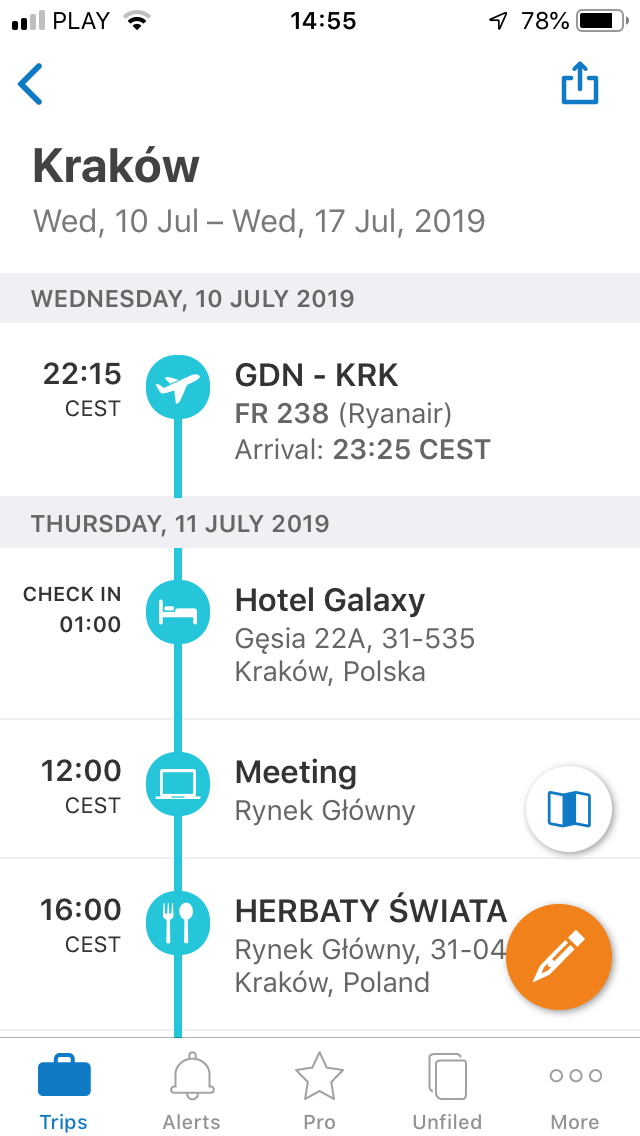
\includegraphics[width=0.9\linewidth, width=5cm]{tripit1}
\caption{Plan podróży.}
\label{fig:TIsubim1}
\end{subfigure}
\begin{subfigure}{0.5\textwidth}
\centering
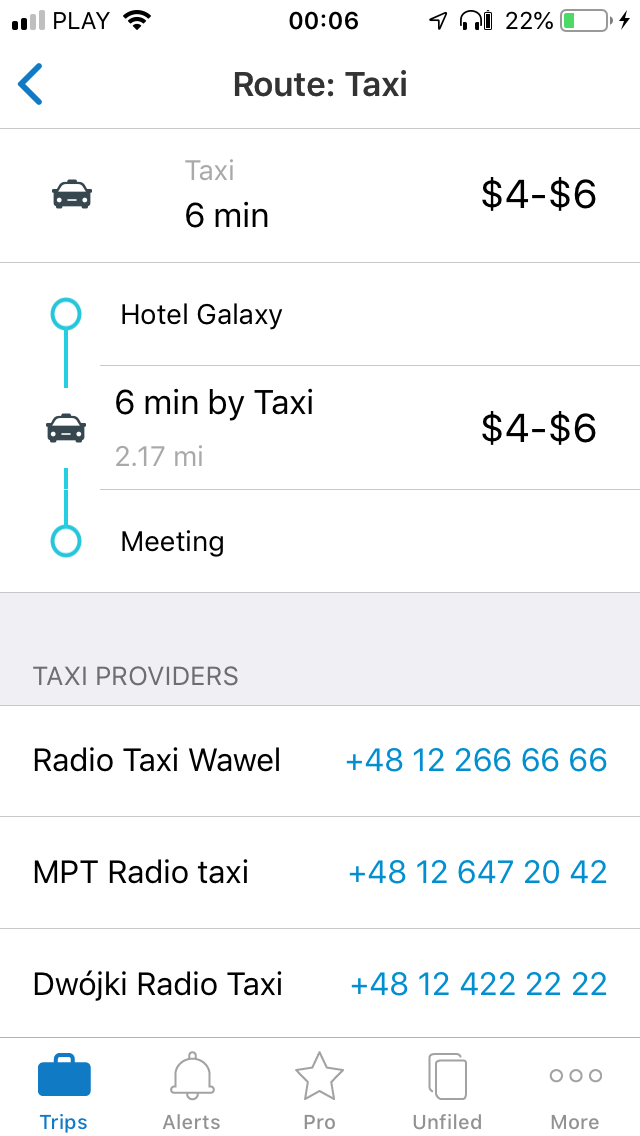
\includegraphics[width=0.9\linewidth, width=5cm]{tripit2}
\caption{Opcje transportu taksówką.}
\label{fig:TIsubim2}
\end{subfigure}
\caption{TripIt: Travel Planner.}
\label{fig:TIimage1}
\end{figure}

\par Oprócz wspomnianego wcześniej automatycznego dodawania rezerwacji i planów przez aplikację po pobraniu tych informacji ze skrzynki pocztowej, można to też było zrobić manualnie. TripIt oferowało 18 różnych elementów, które można było dodać do planu, między innymi: lot (ang. flight), kwatera (ang. lodging), wynajem samochodu (ang. car rental), teatr (ang. theater), rejs (ang. cruise), transport (ang. transportation) i ogólna aktywność (ang. activity). Poszczególne elementy umożliwiały dodanie różnych informacji o planowanej podróży, jednak każdy z nich wymagał dodania daty i godziny do danej aktywności, aby aplikacja mogła je później zorganizować chronologicznie. Przy wpisywaniu niektórych informacji aplikacja podpowiadała jakie słowa mógł mieć na myśli użytkownik, co bywało pomocne. Było tak na przykład w przypadku wpisywania nazwy linii lotniczych i nazwy restauracji, a także w przypadku wybrania pola przeznaczonego na podanie adresu. Była to usługa dostarczana przez firmę Google. Po wybraniu takiego zasugerowanego słowa TripIt często samodzielnie uzupełniał niektóre informacje, takie jak np. adres strony internetowej danego obiektu, czy godzina odprawy samolotowej.
Po dodaniu nowego elementu do planu podróży można go było edytować, usunąć, przenieść do innego planu lub uzupełnić o szczegóły, które nie były dostępne przy tworzeniu np. informacje o rezerwacji (ang. booking info), zdjęcia (ang. photos), uczestnicy (ang. attendees). Dla każdego elementu dostępny był również nawigator (ang. navigator), który po wybraniu miejsca startowego i docelowego wyszukuje możliwe opcje transportu z szacowanym czasem ich trwania i kosztem (w dolarach). Po wybraniu transportu samochodem lub pieszo, aplikacja TripIt przekierowywała do aplikacji Google Maps, gdzie można było zobaczyć wyznaczoną trasę.

\par Ciekawą funkcją było pozyskiwanie informacji o okolicy (ang. neighborhood info), w której znajdował się dodany obiekt. Usługa ta była dostarczana przez GeoSure i udostępniała wskaźniki między innymi z takich kategorii jak: ogólne bezpieczeństwo (ang. overall safety), ryzyko doznania krzywdy fizycznej (ang. physical harm), ryzyko kradzieży (ang. theft). Poza tym TripIt oferowała też wyświetlenie miejsc, będących w pobliżu obiektu z kilku kategorii: restauracje, kawiarnie, bary, bankomaty, parkingi. Wyszukane miejsca pokazywały się na mapie, a po wybraniu jednego z nich można było między innymi zobaczyć godziny otwarcia oraz dodać je do swojego planu podróży.

\begin{figure}[h]
\begin{subfigure}{0.5\textwidth}
\centering
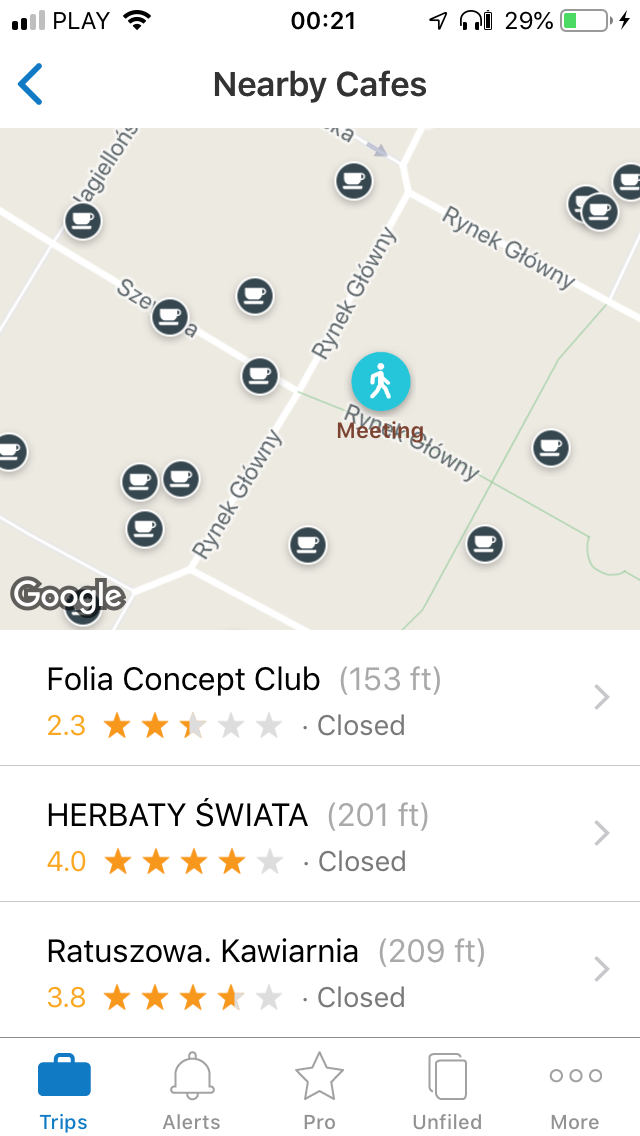
\includegraphics[width=0.9\linewidth, width=5cm]{tripit3}
\caption{Wyszukanie pobliskich kawiarni.}
\label{fig:TIsubim3}
\end{subfigure}
\begin{subfigure}{0.5\textwidth}
\centering
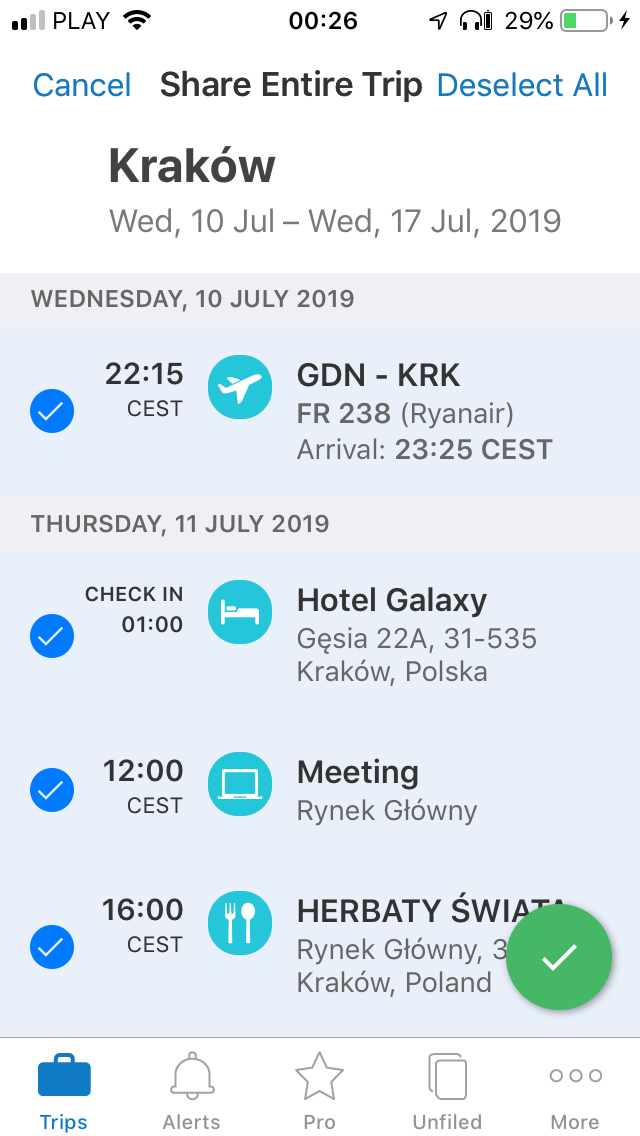
\includegraphics[width=0.9\linewidth, width=5cm]{tripit4}
\caption{Udostępnianie planu podróży.}
\label{fig:TIsubim4}
\end{subfigure}
\caption{TripIt: Travel Planner.}
\label{fig:TIimage2}
\end{figure}

\par Każdy plan lub element podróży można było udostępnić lub zapisać w formacie txt. Wybierając opcję Invite Others to View Trip, plan podróży wysyłano na wybrany adres mailowy (który może zostać wyszukany poprzez kontakty) osoby, której można nadać jedno z trzech uprawnień: can view, can edit, can edit and is traveling. W tak wysłanej wiadomości znajdował się link do planu podróży wraz z mapą, które można było wyświetlić w przeglądarce lub aplikacji. W przeglądarce wyświetlała się dodatkowo informacja o pogodzie na każdy dzień podróży. Osoby, którym nadano odpowiednie uprawnienia i posiadały one konto w serwisie TripIt, mogły edytować udostępniony im plan podróży.

\par W aplikacji można było przechowywać informacje o swoich dokumentach i kontaktach, które mogły się przydać w razie nieprzewidzianych sytuacji. Dane te były dostępne po wprowadzeniu 4-cyfrowego pinu, który należało uprzednio ustawić. W ustawieniach można było włączyć synchronizację kalendarza na naszym urządzeniu z aplikacją TripIt, co powodowało automatyczne dodawanie informacji o planie podróży z aplikacji do kalendarza. Dodatkowo w aplikacji można było obejrzeć statystyki ze wszystkich swoich podróży, takie jak liczba przebytych kilometrów, liczba odwiedzonych krajów i inne.

\par Opisane wyżej funkcje dotyczyły darmowej wersji aplikacji TripIt. Wersja Pro rozszerzała tą wersję przede wszystkim o rozbudowany system powiadomień oraz mechanizmów śledzących (ang. trackers). Niektóre z tych udogodnień to: powiadomienia o dostępności lepszych miejsc w samolocie, przypomnienia o konieczności odprawy 24 godziny przed wylotem, wyszukiwanie alternatywnych połączeń, wysyłanie informacji o locie w czasie rzeczywistym podczas całej podróży, udostępnianie interaktywnych map lotniska. Wersję TripIt Pro można było przetestować za darmo przez 30 dni.

\par Aplikacja TripIt oferowała wiele możliwości w planowaniu swoich podróży, co pozwalało na stworzenie bardzo szczegółowych planów. Wiele informacji trzeba było wprowadzać samodzielnie, jednak aplikacja często podpowiadała jakie słowa mógł mieć na myśli użytkownik, co znacznie ułatwiało i przyspieszało ten proces. Dodatkowym ułatwieniem była funkcja automatycznego dodawania danych o rezerwacjach, które mogły być pobierane ze skrzynki pocztowej. Dużą zaletą aplikacji była również opcja wyznaczania trasy między dwoma punktami, jednak koszt takiej wyprawy podawany był tylko w dolarach amerykańskich bez względu na kraj, w którym odbywała się podróż i miejsce zamieszkania użytkownika. TripIt pozwalała w łatwy sposób wyszukać sąsiednie obiekty, takie jak restauracje, czy parkingi, jednak brakowało tu atrakcji turystycznych, a odległość od tych obiektów podawana była w stopach (ft) i nie dało się tego zmienić. Z pewnością przydatną funkcją była możliwość udostępnienia stworzonego przez siebie planu innym osobom, jednak by wysłać link ze sformatowanym planem można było to zrobić jedynie na adres mailowy, a nie przez inne środki komunikacji, gdzie wysłany plan był dostępny wyłącznie w formie tekstowej. Wadą aplikacji była jej dostępność jedynie w języku angielskim. Ponadto cena wersji PRO, która wprowadzała szereg dodatkowych udogodnień, była wysoka i mogła odstraszać potencjalnego użytkownika.

\section{Aplikacja Google Trips - Travel Planner (Karolina Makuch)}

\par Aplikacja Google Trips – Travel Planner była dostępna na urządzenia mobilne z systemem iOS oraz Android. Była jedną z popularniejszych aplikacji w Sklepie PLAY. Google Trips była także dostępne w Apple Store. 
\par W celu korzystania z Google Trips należało posiadać konto Google. Umożliwiło to dostęp do planu podróży z różnych urządzeń. Niestety aplikacja miała jeden wariant językowy (język angielski).
\par Na samym początku należało wybrać miasto docelowe. Po wyszukaniu miasta, użytkownik miał możliwość nazwania swojej wycieczki oraz dodawania poszczególnych etapów podróży, uwzględniając przedział czasu poświęcony na każdy z nich.

\begin{figure}[h]
\begin{subfigure}{0.5\textwidth}
\centering
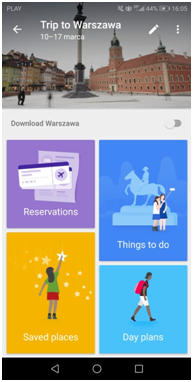
\includegraphics[width=0.9\linewidth, width=5cm]{googletrips1}
\caption{Tworzenie nowej podróży}
\label{fig:GTsubim1}
\end{subfigure}
\begin{subfigure}{0.5\textwidth}
\centering
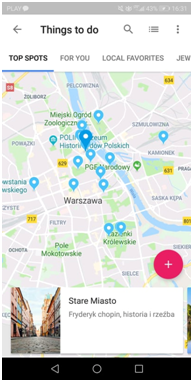
\includegraphics[width=0.9\linewidth, width=5cm]{googletrips2}
\caption{Przeglądanie mapy z polecanymi obiektami}
\label{fig:GTsubim2}
\end{subfigure}
\caption{Google Trips - Travel Planner.}
\label{fig:GTimage1}
\end{figure}

\par Aplikacja umożliwiała zapisywanie rezerwacji (ang. Reservations) lotu (ang. Flight), hotelu (ang. Hotel), pociągu (ang. Train), autobusu (ang. Bus), samochodu (ang. Car rental) oraz restauracji (ang. Restaurant). W zależności od rodzaju transportu użytkownik uzupełniał odpowiednie informacje takie jak: skąd chce się wybrać, dokąd, kiedy, o której godzinie, numer telefonu, numer potwierdzający, miejsca pasażerów oraz rodzaj transportu. Google Trips posiadał także Notatnik posiadający ograniczenie do 10 000 słów.
\par Kolejną opcją była możliwość przejrzenia oraz zapisania dostępnych atrakcji (ang. Things to do). Zostały one podzielone na kilka podkategorii na przykład : polecane (ang. Top Spots), preferowane (ang. For you), parki (ang. Parks \& gardens), muzea (ang. Museums), w pomieszczeniu (ang. Indoors), na świeżym powietrzu (ang. outdoor), przyjazne dzieciom (ang. Kids friendly) oraz okoliczne atrakcje (ang. Farther away). Po wybraniu interesującej użytkownika atrakcji użytkownik mógł zobaczyć fotografię, która została wykonana atrakcji, a także miał możliwość przeczytania opisu oraz recenzji użytkowników. Umieszczony był także adres, numer telefonu oraz adres strony internetowej. Aplikacja umożliwiała także nawigację do danej atrakcji. Po naciśnięciu mapy (górny prawy róg) użytkownik mógł zobaczyć lokalizację atrakcji na planie miasta. Daną atrakcję można było zapisać na jednej z domyślnych list: ulubione(ang. favorites), planowane do odwiedzenia (ang. Want to go) oraz ocenione (ang. starred place). Istniała także możliwość stworzenia własnej listy poprzez podanie nazwy.

\par Następny kafelek umożliwiał przejrzenie zapisanych wcześniej atrakcji oraz wyświetlenie ich w wspomnianych wcześniej listach.

\par Aplikacja układała także sugerowane plany dnia (ang. Day plans). Każdy z nich otrzymał własną nazwę. Składał się z mapy, a także ilości oraz odnośników do poszczególnych atrakcji. Aplikacja udzielała użytkownikowi wskazówek odnośnie godzin i dni otwarcia danych atrakcji, ile czasu zazwyczaj spędzają tam zwiedzający, a także jak dużo czasu zajmuje przejście do kolejnego punktu z planu.

\begin{figure}[h]
\begin{subfigure}{0.5\textwidth}
\centering
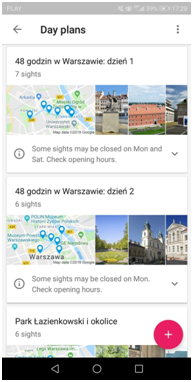
\includegraphics[width=0.9\linewidth, width=5cm]{googletrips3}
\caption{Przeglądanie planu dnia}
\label{fig:GTsubim3}
\end{subfigure}
\begin{subfigure}{0.5\textwidth}
\centering
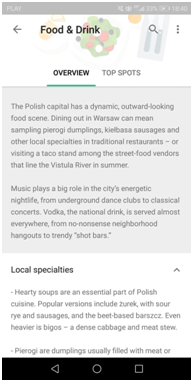
\includegraphics[width=0.9\linewidth, width=5cm]{googletrips4}
\caption{Przeglądanie informacji na temat regionalnej kuchni}
\label{fig:GTsubim4}
\end{subfigure}
\caption{Google Trips - Travel Planner.}
\label{fig:GTimage2}
\end{figure}

\par Korzystanie z aplikacji umożliwiało użytkownikom otrzymanie zniżek na poszczególne usługi na przykład: taksówki (ang. pre-booked taxis) czy wypożyczenie samochodu (ang. car hire).
Aplikacja posiadała także informacje na temat lokalnej kuchni (kafelek Food \& Drink). Zawierał on krótki opis charakterystycznej dla danego rejonu kuchni, wypunktowane lokalne specjalności kuchni (ang. local specialities), polecane miejsca do jedzenia „na mieście” (ang. Dining out), a także wskazówki na temat ‘”nocnego życia” (ang. Nightlife). Zakładka „Top Spots” zawierała najbardziej polecane miejsca w poszczególnych kategoriach: ekskluzywne posiłki (ang.high-end dining), budżetowe posiłki (ang. on a budget), miejsca przyjazne rodzinom (ang.family-friendly), śniadania i przekąski (ang. breakfast \& brunch), obiady(ang.lunch),posiłki wegetariańskie (ang.vegetarian-friendly), bary (ang.vodka bars), piwowarnie kraftowe (ang.craft beer) oraz kawiarnie tematyczne (ang.themed cafes). Po wybraniu danej kategorii istniała opcja sortowania propozycji według odległości. Można było także przefiltrować wyniki ze względu na godziny otwarcia (ang. Open now) a także wcześniej zapisanych pozycji (ang. only saved places).
\par Kafelek Zwiedzaj (ang. getting around) umożliwiał sprawdzenie poszczególnych kategorii transportu: on arrival (taxi, ride service, train, bus), public transport (ticket, metro, bus, train, tram), taxi (ang. taxi/ride service), driving, walking \& biking. Każda kategoria była wystarczająco szczegółowo opisana. Zawierała informacje na temat cen, możliwości dojazdu, czasu trwania, możliwych korkach oraz na przykład numerów telefonów do taksówek.
\par Aplikacja zawierała także wskazówki związane z zakupami (ang. Need to know). Informowała użytkownika o najpopularniejszych godzinach otwarcia sklepów, gdzie znajduje się ich najwięcej (ang. Shopping districts). Można było tam także znaleźć przykładowe sklepy (ang. Markets) oraz galerie handlowe (ang. Malls).
 
\begin{figure}[h]
\begin{subfigure}{0.5\textwidth}
\centering
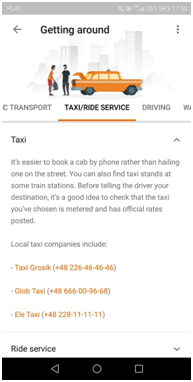
\includegraphics[width=0.9\linewidth, width=5cm]{googletrips5}
\caption{Przeglądanie możliwości transportu}
\label{fig:GTsubim5}
\end{subfigure}
\begin{subfigure}{0.5\textwidth}
\centering
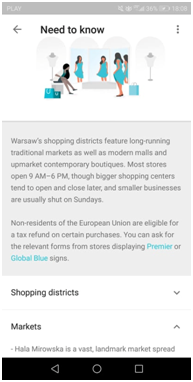
\includegraphics[width=0.9\linewidth, width=5cm]{googletrips6}
\caption{Przeglądanie przydatnych informacji}
\label{fig:GTsubim6}
\end{subfigure}
\caption{Google Trips - Travel Planner.}
\label{fig:GTimage3}
\end{figure}

\par Zaplanowana przez użytkownika wycieczka została automatycznie przypisana do konta Google. Istniała możliwość udostępnienia jej znajomym. Można było połączyć kilka wycieczek. Po pobraniu informacji na temat danej wycieczki, istniała możliwość powrotu do planu, gdy telefon nie miał dostępu do internetu.
\par Niestety aplikacja była dostępna tylko w języku angielskim. Posiadała także kilka innych wad. Przykładowo podczas wyszukiwania odpowiedniego hotelu aplikacja wyświetla listę miejsc, na której mógł znajdować się sklep meblowy. Brakowało także podpowiedzi przy niektórych polach np. cartype. Aplikacja nie zawsze dodawała informacje z serwisu gmail. Nie można było samemu dodać atrakcji za pomocą informacji z Google Maps, a także dodać ręcznie maili z rezerwacjami.

\section{Sygic Travel - Planuj podróż (Anna Malizjusz)}

\par Planowanie podróży umożliwia również aplikacja \textit{Sygic Travel: Planuj Podróż}, która została pobrana z serwisu Google Play. Jej duża zaleta to możliwość korzystania z większości funkcji w języku polskim oraz brak konieczności tworzenia konta. Jedyną opcją niedostępną dla niezalogowanego użytkownika była synchronizacja z innymi urządzeniami.
\par Podstawowymi informacjami potrzebnymi do rozpoczęcia planowania podróży były cel, data rozpoczęcia oraz data zakończenia (rys.~\ref{fig:STsubim1}). Opcjonalnie można było podać miejsce przybycia oraz zakwaterowania. Wygodny wybór daty umożliwił wyświetlany kalendarz, a miejsca należało wybrać z podanej listy. Istniała również możliwość filtrowania podanych miejsc po nazwie.
\par Po stworzeniu podróży został wyświetlony interfejs oferujący różne opcje (rys.~\ref{fig:STsubim2}). Po wybraniu mapy można zobaczyć mapę miejsca docelowego z zaznaczonymi atrakcjami. Listę atrakcji można też zobaczyć wybierając opcję miejsca. W obu przypadkach można wybrać kategorie, np. zwiedzanie, zakupy, relaks oraz tagi, np. zwierzęta mile widziane (ang. pets allowed), a także możliwe było dodanie miejsca do odwiedzenia w danym dniu. Dodatkowo zaprezentowano szacunkowy czas dotarcia do celu piechotą z miejsca zakwaterowania. Ta część aplikacji nie została przetłumaczona i była dostępna tylko w języku angielskim. Analogicznie można było przeglądać dostępne kwatery po wybraniu opcji hotele. Dostępne były typowe opcje pomocne w poszukiwaniu zakwaterowania, takie jak wybór średniej oceny, przyznanych gwiazdek, typu zakwaterowania czy udogodnień, np. darmowe Wi-Fi (ang. free hotel Wi-Fi) lub klimatyzacja (ang. air conditioning).
\begin{figure}[h]
\begin{subfigure}{0.5\textwidth}
\centering
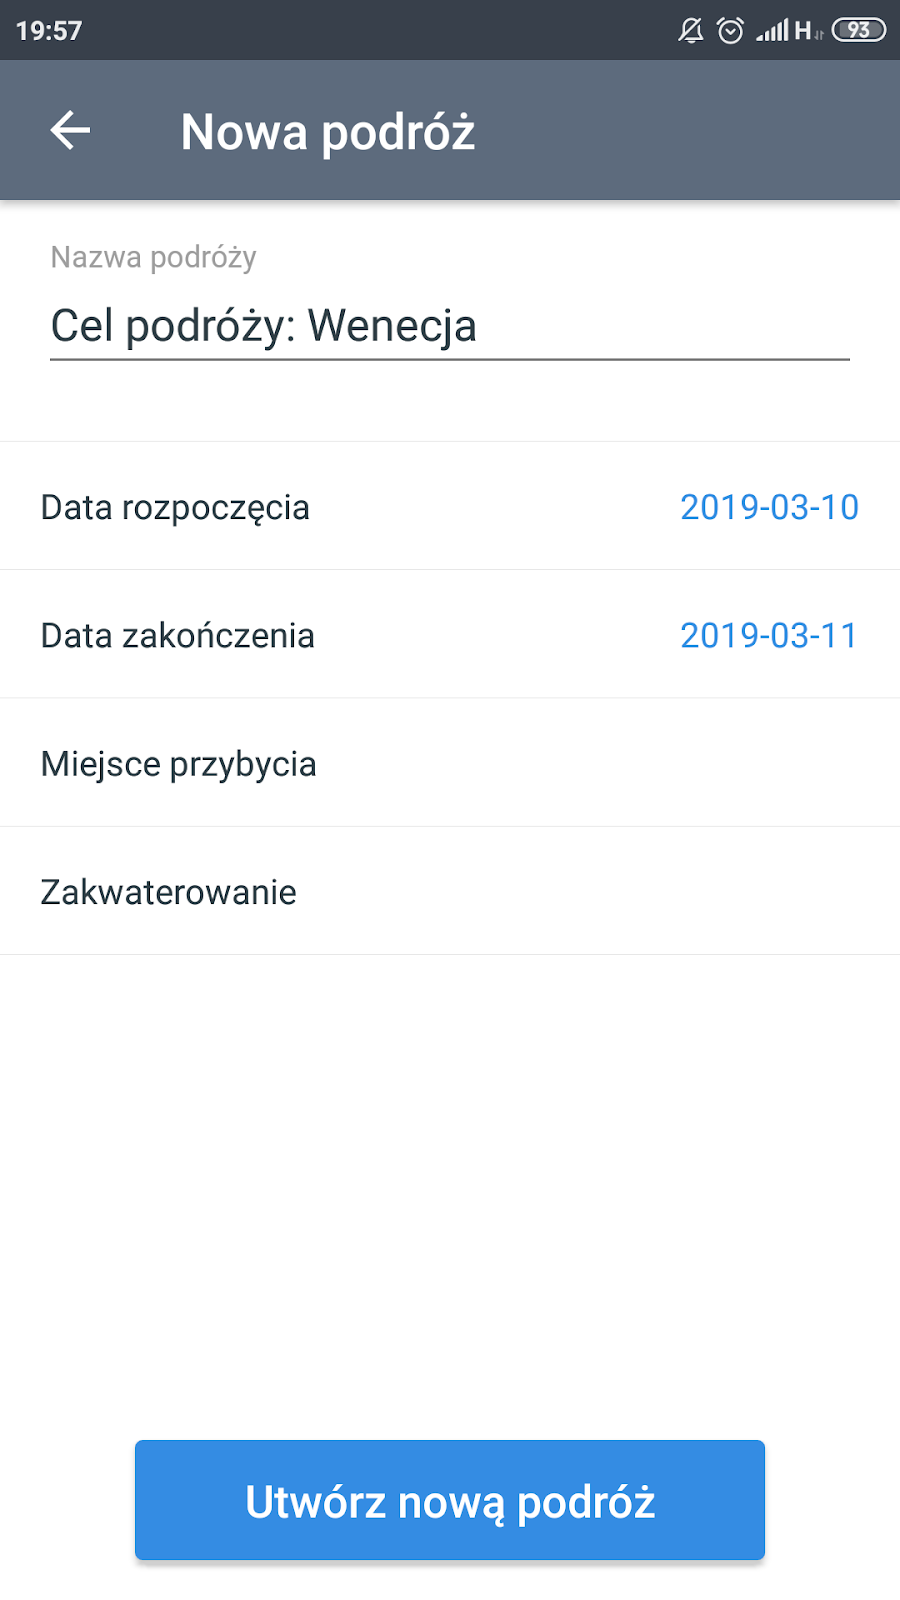
\includegraphics[width=0.9\linewidth, width=5cm]{sygictravel1}
\caption{Tworzenie nowej podróży.}
\label{fig:STsubim1}
\end{subfigure}
\begin{subfigure}{0.5\textwidth}
\centering
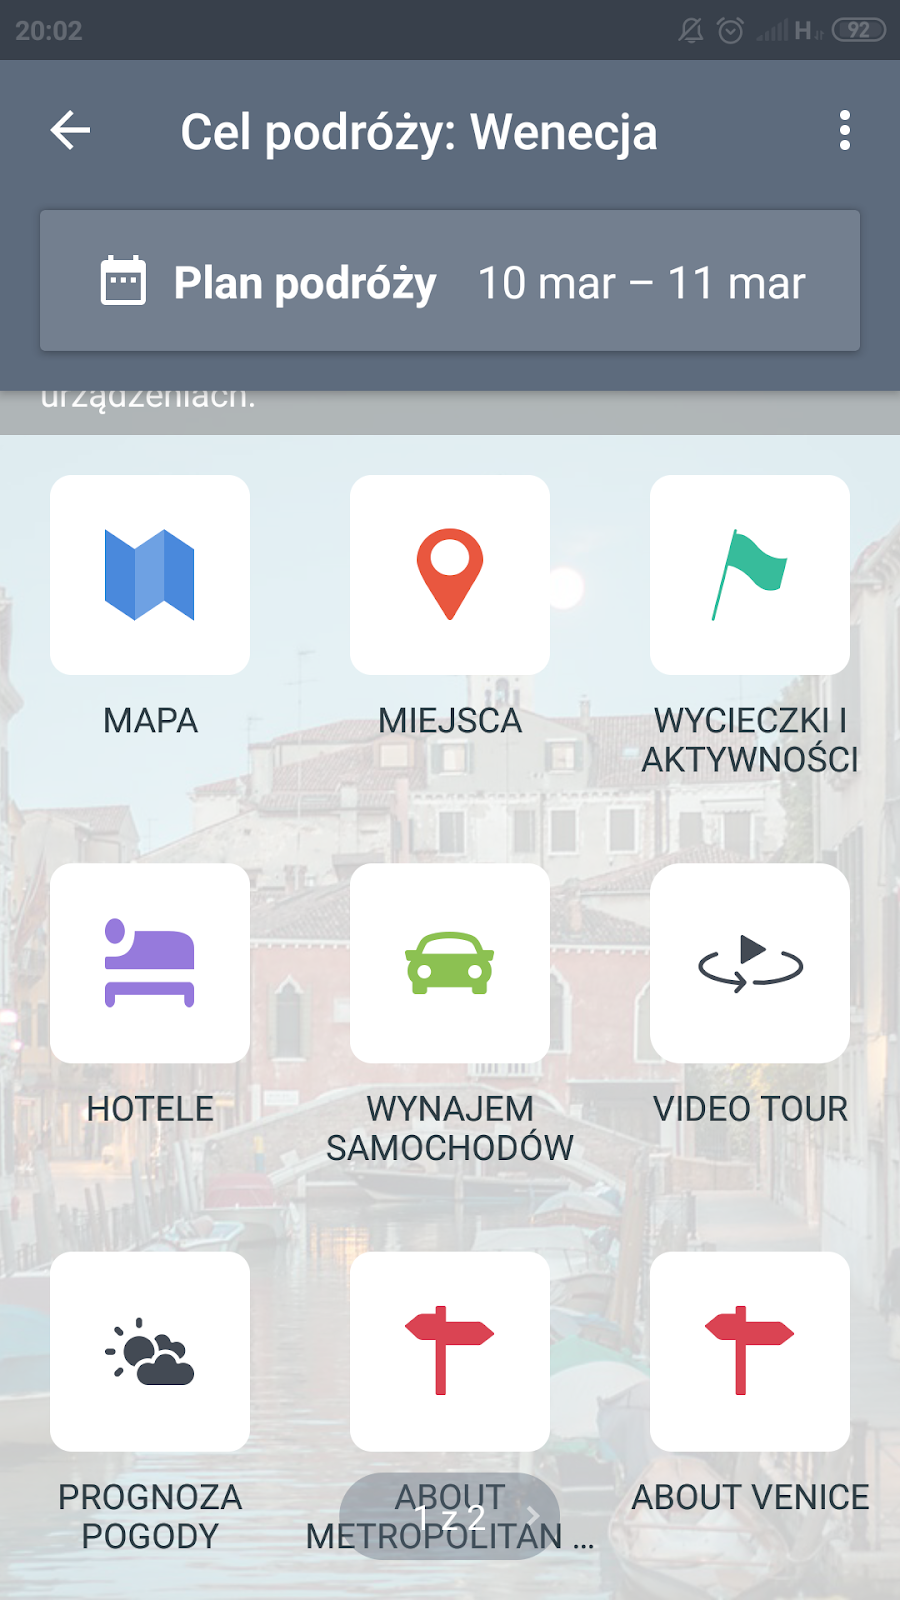
\includegraphics[width=0.9\linewidth, width=5cm]{sygictravel2}
\caption{Menu główne.}
\label{fig:STsubim2}
\end{subfigure}
\caption{Sygic Travel - Planuj podróż.}
\label{fig:STimage}
\end{figure}
\par Innego typu funkcjami aplikacji były wycieczki i aktywności oraz wynajem samochodów. Pierwsza opcja umożliwiała wyszukiwanie wycieczek, a także ich rezerwację oraz płatność. Druga wyszukiwała oferty wynajmu samochodów, wyświetlała wszystkie dostępne informacje oraz umożliwiała rezerwację. W obu funkcjach udostępniono możliwość filtrowania wyników. Poważną wadą wyszukiwarki samochodów do wynajęcia stanowił niejasny komunikat o błędzie w przypadku podania dat z przeszłości, który sugerował sprawdzenie zaznaczonych pól nie wskazując możliwego rozwiązania problemu.
\par Kolejna ciekawa opcja to wycieczka wideo (ang. video tour), która była dostępna tylko dla bardziej popularnych celów podróży. Po wybraniu tej opcji użytkownikowi wyświetlany był film wraz z angielskim komentarzem z jednodniowej wycieczki po wybranym mieście. Prezentowano charakterystyczne i warte odwiedzenia zabytki i atrakcje turystyczne, a użytkownikowi umożliwiono ingerowanie w pokazywany obraz. Filmy oferowały widok 360° po obróceniu telefonu.
\par Trzy kolejne funkcje były czysto informacyjne, lecz przydatne. Pokazywały prognozę pogody na najbliższe 14 dni, a także informacje o mieście i okolicy. Obszerność tych danych różniła się w zależności od popularności celu podróży, ale mogła stanowić dobrą podstawę dla nieobeznanych z miejscem użytkowników. Informacje w języku angielskim zostały zaczerpnięte z serwisu Wikivoyage, który można otworzyć w aplikacji oraz przeglądarce internetowej.
\par Po zakupie \textit{Sygic Travel Premium} za 88,99 zł pojawiały się dodatkowe funkcjonalności, takie jak zapisanie mapy miejsca docelowego do użytku offline. Kolejną opcją było wyświetlenie informacji o zabytkach, hotelach i atrakcjach, których odwiedzenie proponowała aplikacja. Darmowa wersja oferowała wszystkie najbardziej potrzebne opcje, więc zakup rozszerzonej wersji nie był koniecznością, a jedynie nieznacznym zwiększeniem możliwości aplikacji.
\par Aplikacja została zintegrowana z innymi produktami firmy Sygic. Przy każdym miejscu oferowała możliwość nawigacji przy pomocy Sygic GPS Navigation \& Maps, a rezerwacja wycieczek i samochodów była wspierana przez witrynę \textit{Sygic Travel}, która była dostępna również z komputera z przeglądarki internetowej.
\par \textit{Sygic Travel} to spełniające podstawowe funkcje narzędzie ułatwiające planowanie podróży. Nie oferowała wielu możliwości, jednak warto zauważyć, że większość z nich była dostępna w wersji podstawowej i nie zmuszała użytkownika do zakupu stosunkowo drogiej wersji premium. Udostępniała bogaty wybór możliwych do odwiedzenia miejsc w wybranym celu podróży, a sam cel mógł należeć do egzotycznych, np. Udaipur w Indiach. Podstawowe informacje, takie jak mapa, atrakcje turystyczne czy prognoza pogody były zawsze dostępne. 

\section{Expedia (Magdalena Solecka)}
\par Kolejna aplikacja do planowania podróży to \textit{Expedia}, dostępna na urządzeniach z systemem iOS oraz Android. Korzystanie z niej było możliwe po założeniu konta użytkownika. Wśród dostępnych tłumaczeń nie znajdował się język polski. Aplikacja składała się z czterech głównych funkcjonalności: rezerwacja noclegu (ang. Hotels), rezerwacja lotu (ang. Flights), rezerwacja samochodu (ang. Cars) oraz wyszukiwanie ciekawych miejsc w okolicy (ang. Thing to Do). Nie było możliwości wyszukania restauracji w rejonie ani transportu naziemnego, koleją lub autobusem.
\begin{figure}[h]
\begin{subfigure}{0.5\textwidth}
\centering
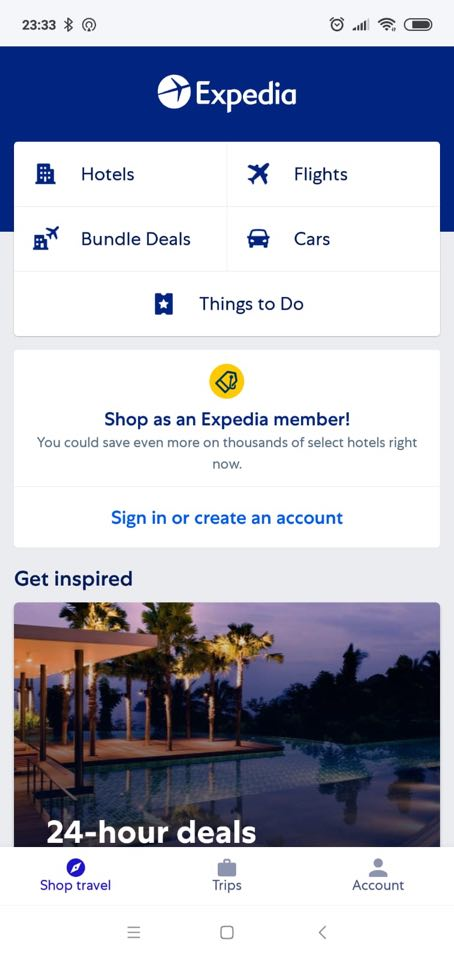
\includegraphics[width=0.9\linewidth, width=5cm]{expedia1}
\caption{Menu główne.}
\label{fig:Esubim1}
\end{subfigure}
\begin{subfigure}{0.5\textwidth}
\centering
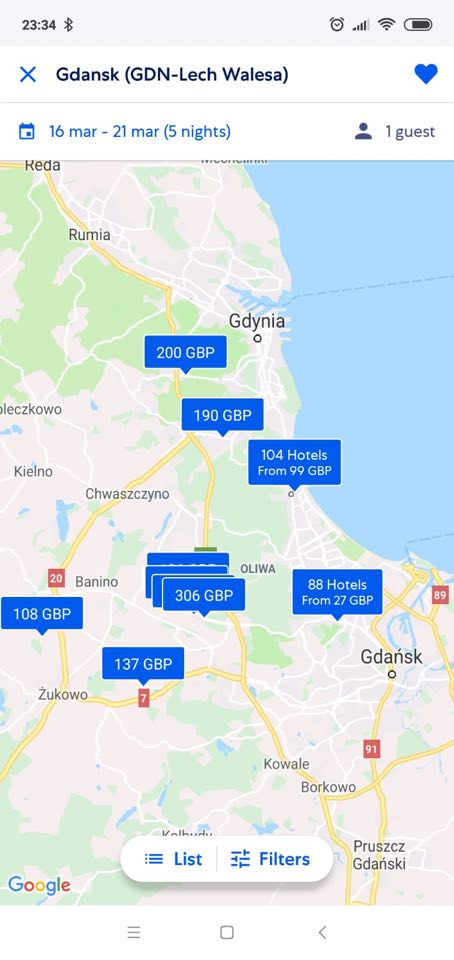
\includegraphics[width=0.9\linewidth, width=5cm]{expedia2}
\caption{Wyszukiwanie noclegu.}
\label{fig:Esubim2}
\end{subfigure}
\caption{Expedia.}
\label{fig:Eimage}
\end{figure}
\par W celu wyszukania noclegu należało podać następujące dane: datę zameldowania i wymeldowania, miasto docelowe podróży, liczbę pokoi oraz osób do zakwaterowania. Zaprezentowane przez aplikację wyniki mogły zostać posortowane po cenie lub recenzjach użytkowników, a także przefiltrowane względem darmowego anulowania rezerwacji, śniadaniu wliczonym w cenę pobytu, klimatyzacją czy Wi-Fi. Wygodnym rozwiązaniem była mapka z naniesionymi na nią punktami z ceną w miejscu, w którym znajdował się oferowany pokój, co umożliwiało łatwiejszą ocenę odległości od centrum.
\par W przypadku rezerwacji miejsca w samolocie można było wyszukać lot w jedną lub obie strony. Należało podać miejsce wylotu i przylotu oraz daty. Przedstawione wyniki można było porządkować według rosnącego kosztu. Aplikacja nie dawała możliwości porównania cen w różnych dniach np. w formie kalendarza uzupełnionego najniższymi cenami w danym dniu, co przy podróżowaniu z niskim budżetem byłoby pomocne. Możliwe było równoczesne wyszukanie lotów oraz noclegu (ang. Bundle Deals).
\par Aplikacja oferowała również możliwość wypożyczenia samochodu. Tak jak w poprzednich dwóch przypadkach należało podać przedział czasu korzystania z pojazdu, miejsce odbioru i pozostawienia. Wyświetlone informacje o pojazdach były przydatne przy dokonywaniu wyboru, automatyczna czy manualna skrzynia biegów, ilość pasażerów.Dostępne sortowanie po cenie.
\par Ostatnia funkcjonalność, wyszukiwanie atrakcji, zabytków, ciekawych wydarzeń. Wymagane ramy czasowe oraz lokalizacja. Rezultaty mogły być przeglądane po cenie lub popularności. Nie umożliwiono użytkownikowi oceny odległości między zaproponowanymi miejscami tak jak w przypadku noclegu, ale pomocny był przybliżony czas, który należy przeznaczyć na każdą z atrakcji.
\par Wszystkie rezerwacje wykonane za pomocą aplikacji \textit{Expedia}, można było przeglądać w zakładce Wycieczki (ang. Trips) i takim zestawem dzielić się ze współtowarzyszami podróży również korzystających z aplikacji.

\chapter{Specyfikacja wymagań systemowych - ekstrakt (Anna Malizjusz)}
\par W celu lepszego zrozumienia wymagań projektu inżynierskiego przygotowano dokument SWS (Specyfikacji Wymagań Systemowych) w całości umieszczony na załączonej do pracy płycie~CD. Dokonano identyfikacji udziałowców projektu i otoczenia systemu z uwzględnieniem użytkowników oraz systemów zewnętrznych. Wyróżniono cele projektu oraz wymagania, których spełnienie będzie kluczowe dla końcowej akceptacji systemu. Poniżej przedstawiono najistotniejsze elementy SWS, które miały największy wpływ na projekt i~implementację systemu.
\newline
\newline
\noindent Wyróżniono udziałowców, których wpływ na system powinien być największy:

\begin{itemize}
\item programiści,
\item promotor,
\item użytkownik.
\end{itemize}

\noindent A także dokumenty, które należało uwzględnić w pracy:

\begin{itemize}
\item regulamin aplikacji,
\item rozporządzenie o ochronie danych osobowych (RODO).
\end{itemize}

\par Docelowego użytkownika zidentyfikowano jako młodego człowieka, najczęściej studenta o ograniczonym budżecie i czasie, który może poświęcić na planowanie podróży. Posiada on smartfona z dostępem do internetu oraz używa systemu operacyjnego Android. Chce podróżować i kontaktować się z przyjaciółmi poprzez aplikację. Często zapomina o terminach i~koniecznych dokumentach, więc potrzebuje przypomnień oraz dostępu do skanów przy pomocy telefonu.

\par Wyróżniono systemy zewnętrzne, z którymi zintegrowano aplikację. Skupiono się na dostępie do zewnętrznego API udostępnionego przez serwis Here \cite{Here}, które umożliwiało dostęp do map, nawigacji i wyszukiwania obiektów takich jak hotele, restauracje, zabytki, itp. Zaletą serwisu był darmowy dostęp do danych. Here umożliwiało wykonanie 250 tys. zapytań miesięcznie bez dodatkowych opłat, a każdy kolejny tysiąc kosztował 1\$, co zostało uznane za wystarczające dla testowania aplikacji. Uwzględniono również system GPS, który był niezbędny do zrealizowania podstawowych funkcjonalności, np.~wyszukiwania obiektów w pobliżu aktualnej lokalizacji. W tym celu zdecydowano skorzystać z możliwości oferowanych przez serwis Google Play w paczce \textit{com.google.android.gms.location}\cite{gms.location}.

\par
\noindent \newline Określono najważniejsze cele projektu:

\begin{itemize}
\item zwiększenie zadowolenia z podróży,
\item zaspokajanie potrzeb informacyjnych użytkowników,
\item zoptymalizowanie trasy,
\item zmniejszenie ilości spóźnień,
\item ułatwienie komunikacji pomiędzy użytkownikami,
\item ułatwienie możliwości koordynacji planu dnia przez użytkownika,
\item skrócenie czasu oczekiwania na dany środek transportu,
\item zmniejszenie czasu przeznaczonego na planowanie podróży,
\item zmniejszenie poziomu stresu użytkowników podczas planowania podróży.
\end{itemize}

\par
\noindent\newline Zidentyfikowano wymagania funkcjonalne, które jednocześnie stanowiły kryteria akceptacyjne projektu: 

\begin{itemize}
\item rejestracja i logowanie użytkownika,
\item dodanie, przeglądanie i edycja planu podróży i planu dnia,
\item wyszukanie elementu w pobliżu danej lokalizacji,
\item wyszukanie zakwaterowania,
\item wyszukanie i zaproszenie innego użytkownika do wyświetlania lub edycji podróży,
\item dodanie oceny do planu dnia, podróży lub odwiedzonego miejsca,
\item otrzymanie propozycji na podstawie ocen,
\item wyszukanie transportu między lokalizacjami,
\item wyszukanie najkrótszej trasy,
\item skanowanie biletów i innych dokumentów potrzebnych w trakcie podróży.
\end{itemize}

\par
\noindent Wyróżniono dodatkowe wymagania, które nie były niezbędne do realizacji projektu, ale znacznie zwiększały możliwości aplikacji: 

\begin{itemize}
\item oznaczenie elementu z planu dnia jako wykonany,
\item udostępnianie zrealizowanego punktu planu dnia w mediach społecznościowych,
\item wygenerowanie planu dnia/podróży,
\item zapisywanie podróży i dokumentów na urządzeniu, aby możliwe było korzystanie z nich bez dostępu do internetu,
\item powiadomienie o obiekcie w okolicy,
\item powiadomienie o opóźnieniu,
\item powiadomienia dotyczące lotów,
\item przeglądanie statystyk zrealizowanych podróży.
\end{itemize}

\par Dodatkowo zostały określone wymagania jakościowe dotyczące aplikacji. Ze względu na RODO przetwarzanie danych użytkowników ograniczono do minimum i~zdecydowano o wyświetlaniu użytkownikom informacji o sposobie używania danych. Postanowiono skorzystać z bezpiecznych algorytmów szyfrowania i uwierzytelniania, aby zapewnić danym bezpieczeństwo. 
Zobowiązano się do zapewnienia autentyczności proponowanych podróży, tj. sugerowany czas spędzony w danym obiekcie jest zbliżony do rzeczywistego i trafności polecanych obiektów. Zapytania użytkowników mają być obsługiwane nie dłużej niż 5~s., a układanie planu dnia będzie trwać maksymalnie 10~s.

\par Za docelowe urządzenie przyjęto smartfon z systemem operacyjnym Android, którego minimalna wersja to 5.0 (Lollipop), co miało zapewnić obsługę ponad 94\% urządzeń z systemem Android (dane aktualne na dzień 05.05.2019\cite{Android usage}). Spodziewane wymiary urządzeń to od~115.20~mm~x~58.60~mm do~242,8~mm~x~189,7~mm. Zaplanowano rozszerzenie działania aplikacji na telefony z systemem operacyjnym iOS.

\par Zwrócono uwagę na zagwarantowanie czytelności interfejsu użytkownika. Zaplanowano użycie stonowanych, niejaskrawych kolorów i ograniczenie dostępnych informacji na jednym ekranie z możliwością przejścia do kolejnych stron lub filtrowania wyników. Dostępne ma być powiększenie ekranu.

\chapter{Projekt systemu (Magdalena Solecka)}
\par System postanowiono podzielić na następujące komponenty:
\begin{itemize}
\item Po stronie serwera:
\begin{itemize}
\item Podsystem planowania (ang. Planning subsystem)
\item Podsystem wyszukiwania (ang. Search subsystem)
\item Podsystem zarządzania danymi użytkownika (ang. User Data Management Subsystem)
\item Podsystem polecający (ang. Recommendation Subsystem)
\item Podsystem usług społecznościowych (ang. Social Services Subsystem)
\item Podsystem zarządzania (ang. Management Subsystem)
\end{itemize}
\item Po stronie aplikacji mobilnej:
\begin{itemize}
\item GUI
\item Prezenter (ang. Presenter)
\item Podsystem zarządzania plikami (ang. File Management Subsystem)
\item Podsystem skanowania (ang. Scanning Subsystem)
\end{itemize}
\end{itemize}
\par Kontakt klienta mobilnego z aplikacją serwerową zaplanowano poprzez interfejs komunikacji (ang. communication interface). Zależności pomiędzy podsystemami zostały przedstawione na diagramie (rys.~\ref{fig:subsystems}).

\indent\newline
\begin{figure}[h]
\centering
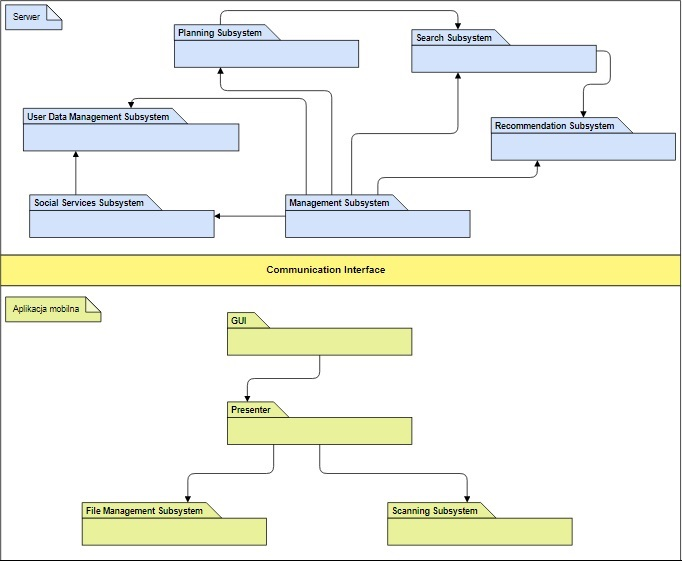
\includegraphics[width=\linewidth]{subsystems}
\caption{Diagram komponentow systemu.}
\label{fig:subsystems}
\end{figure}

\section{Scenariusze użycia}
\par Zaprojektowano scenariusze użycia w celu dokładnego określenia sposobów, na które użytkownicy będą korzystać z aplikacji. Wyróżniono najważniejsze:
\begin{enumerate}
  \item Stworzenie planu dnia.
  \item Wygenerowanie planu dnia.
  \item Stworzenie planu podróży.
  \item Interakcje z innymi użytkownikami aplikacji.
  \item Interakcje serwera z aplikacją w czasie trwania podróży.
\end{enumerate}

\subsection{Stworzenie planu dnia (Magdalena Solecka)}
\par Martyna widzi pusty ekran planu dnia. Wpisuje miasto docelowe wyjazdu - Paryż. Wybiera przycisk "+" i wybiera atrakcje. Ukazuje się przed nią ekran wyszukiwania ze znakiem wyszukiwania, a po chwili z wynikami wyszukiwania w formie listy atrakcji. Wybiera jeden z elementów listy – katedra Notre Dame i czyta jej opis. Wybiera przycisk "Dodaj". Widzi ponownie ekran planu Dnia z dodaną przez siebie atrakcją. Wybiera w ten sposób kilka kolejnych atrakcji. Ponownie wybiera przycisk "+" i wybiera restauracje. Ponownie widzi ekran wyszukiwania z listą restauracji. Wybiera pasujący jej obiekt i przy użyciu przycisku "Dodaj" zostaje on dodany do  planu dnia który ponownie wyświetla się przed nią. Użytkownik wybiera przycisk "Ułóż" i czeka aż aplikacja zakończy obliczanie najbardziej optymalnej trasy. Po kilku sekundach plan dnia jest już gotowy. Martyna stwierdza jednak że potrzebuje w ciągu dnia odpoczynku dlatego postanawia przesunąć zwiedzanie katedry Notre Dame na następny dzień. Wybiera element z katedrą i przycisk "Przenieś", a następnie numer dnia podróży. Następnie stwierdza, że właściwie nie interesuje jej sztuka sakralna, więc usuwa element z planu przesuwając go w prawo.

\noindent\newline Warunki początkowe:
\begin{enumerate}
  \item Użytkownik jest zalogowany.
  \item Aplikacja ma dostęp do internetu.
  \item Użytkownik wybrał opcję stwórz plan dnia.
\end{enumerate}

\par
\noindent\newline
Warunki końcowe:
\begin{enumerate}
  \item Użytkownik stworzył plan dnia.
\end{enumerate}

\noindent\newline
\begin{figure}[h]
\centering
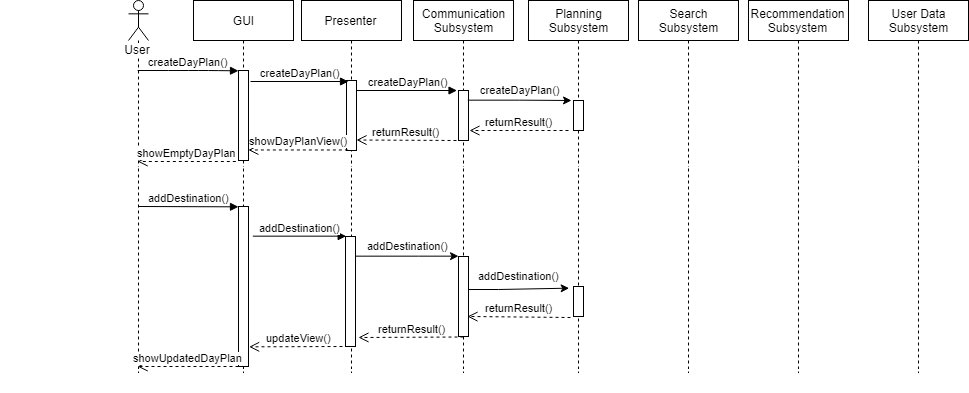
\includegraphics[width=\linewidth]{dayPlan1}
\caption{Tworzenie planu dnia(1).}
\label{fig:dayPlan1}
\end{figure}
\begin{figure}[h]
\centering
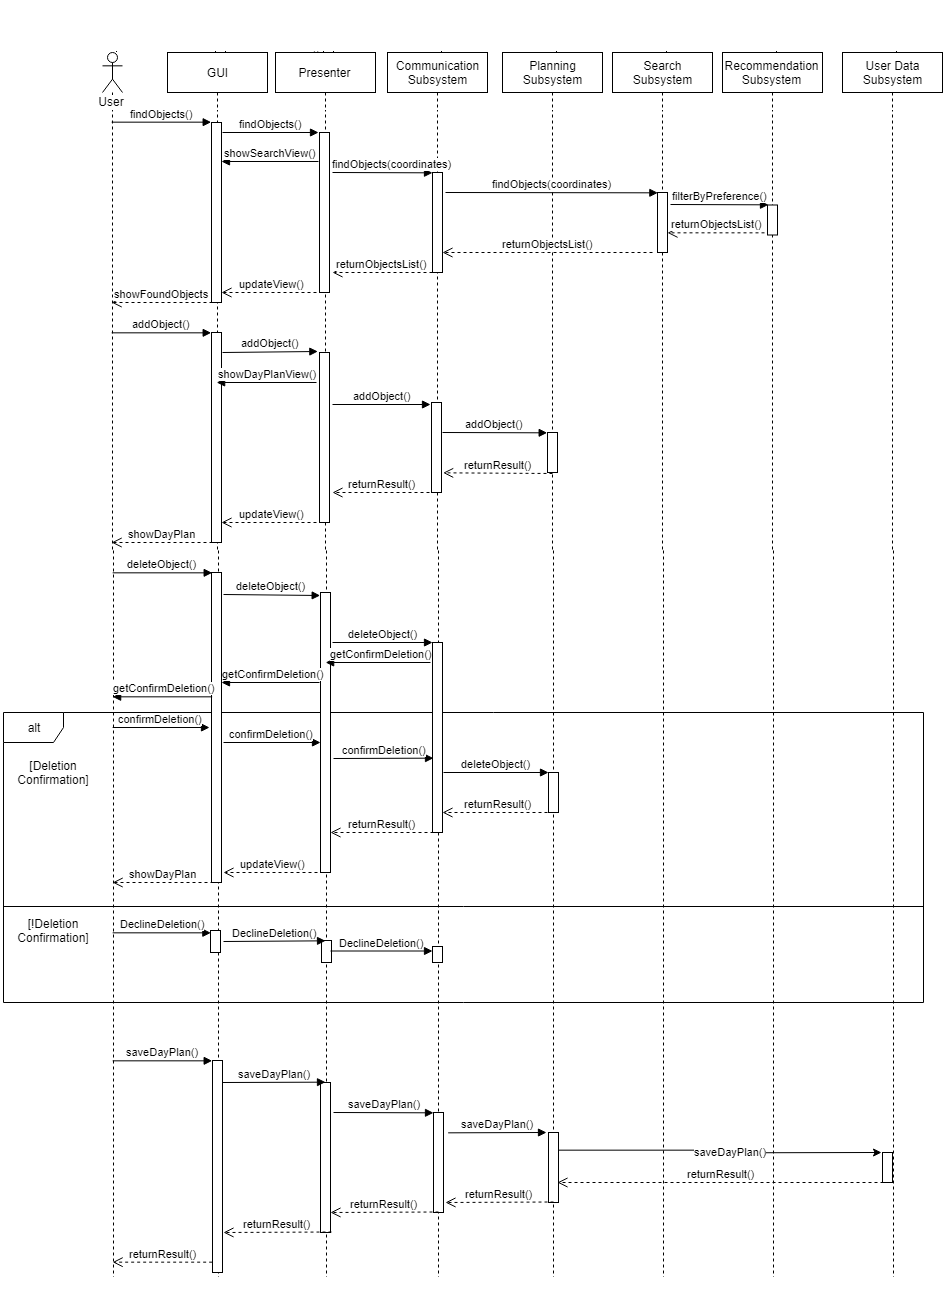
\includegraphics[width=\linewidth]{dayPlan2}
\caption{Tworzenie planu dnia(2).}
\label{fig:dayPlan2}
\end{figure}
\FloatBarrier

\subsection{Wygenerowanie planu dnia (Anna Malizjusz)}
\par Martyna stworzyła wyjazd, lecz nie ma pomysłu na spędzenie dnia. Wybiera w aplikacji swoją podróż, po czym generuje przyciskiem plan dnia. Zostaje wyświetlony rezultat, który może dowolnie modyfikować. (rys.~\ref{fig:generateDayPlan}).

\noindent Warunki początkowe:
\begin{enumerate}
  \item Użytkownik jest zalogowany.
  \item Aplikacja ma dostęp do internetu.
  \item Użytkownik wybrał podróż.
\end{enumerate}
\par
\noindent\newline
Warunki końcowe:
\begin{enumerate}
  \item Wyświetlono proponowany plan podróży.
\end{enumerate}

\noindent\newline
\begin{figure}[h]
\centering
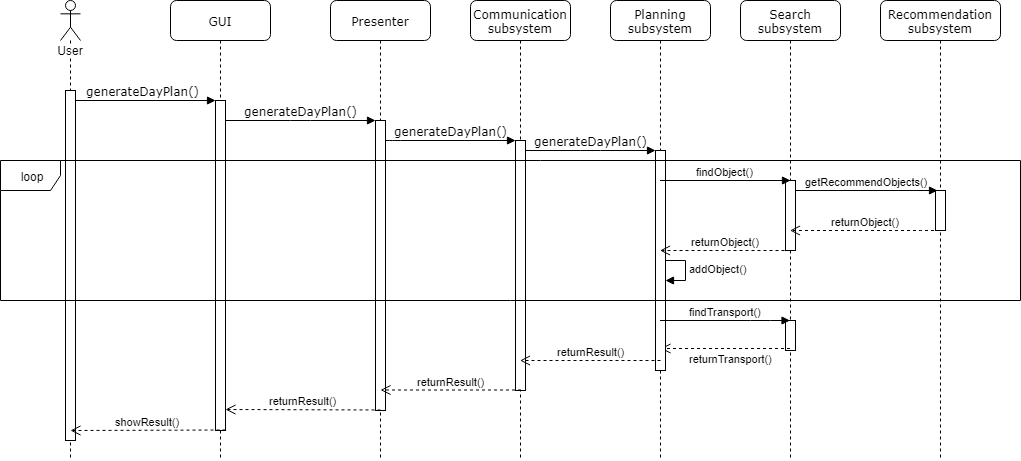
\includegraphics[width=\linewidth]{generateDayPlan}
\caption{Generowanie planu dnia.}
\label{fig:generateDayPlan}
\end{figure}
\FloatBarrier


\subsection{Stworzenie planu podróży (Karolina Makuch)}
\FloatBarrier
\par Martyna pragnie zaplanować podróż za pomocą aplikacji poprzez aplikację podróż.  (rys.~\ref{fig:addTravel}).

\noindent\newline Warunki początkowe:
\begin{enumerate}
  \item Użytkownik jest zalogowany.
  \item Aplikacja ma dostęp do internetu.
  \item Użytkownik wybrał opcję stwórz plan podróży.
\end{enumerate}
\par
\noindent\newline
Warunki końcowe:
\begin{enumerate}
  \item Użytkownik stworzył plan podróży.
\end{enumerate}

\noindent\newline
\begin{figure}[h]
\centering
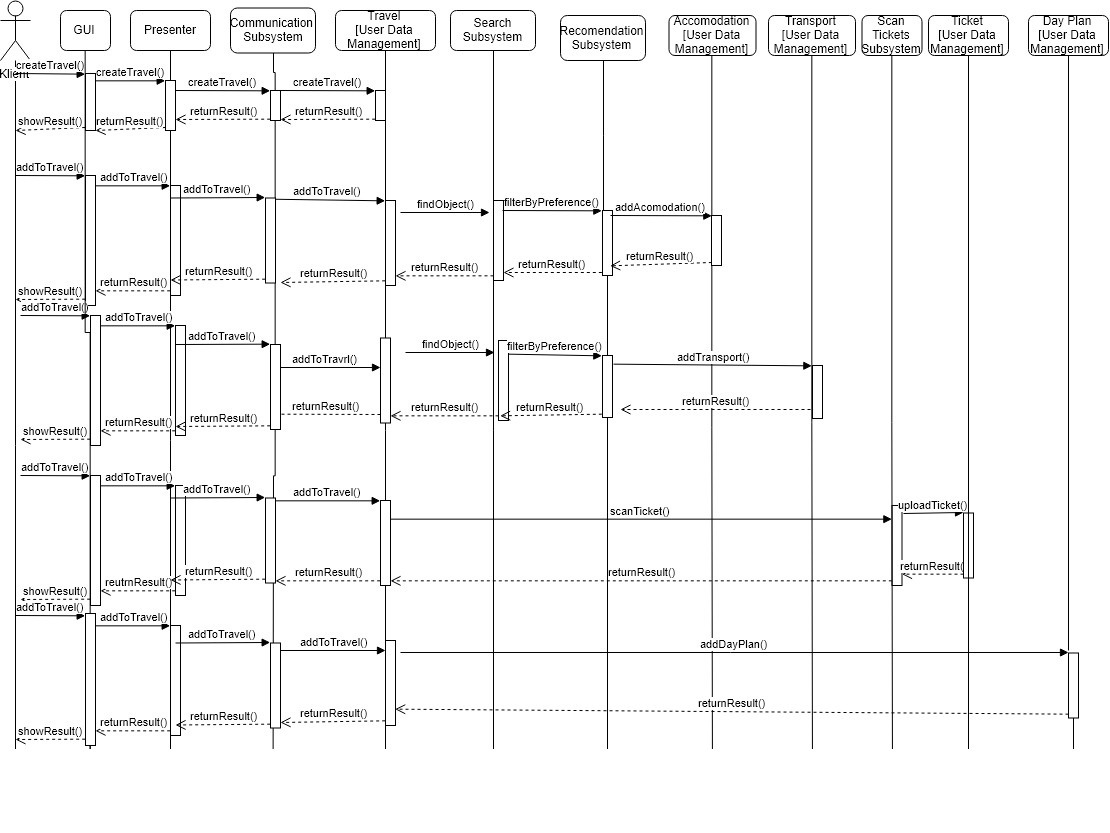
\includegraphics[width=\linewidth]{addTravel}
\caption{Tworzenie planu podróży.}
\label{fig:addTravel}
\end{figure}

\FloatBarrier
\subsection{Interakcje z innymi użytkownikami aplikacji (Anna Malizjusz)}
\par Martyna wyjeżdża na wakacje razem z~koleżanką, więc chce udostępnić jej swój plan podróży. Zaprasza nowego użytkownika do skorzystania z aplikacji (rys.~\ref{fig:inviteFriend}), po czym dodaje znajomego (rys.~\ref{fig:addFriend}) i~zaprasza koleżankę do edytowania podróży (rys.~\ref{fig:shareTravel}).
\FloatBarrier
\subsubsection{Zapraszanie użytkownika do aplikacji}

\noindent Warunki początkowe:
\begin{enumerate}
  \item Użytkownik jest zalogowany.
  \item Aplikacja ma dostęp do internetu.
  \item Użytkownik wybrał z menu opcję "Znajomi".
\end{enumerate}
\par
\noindent\newline
Warunki końcowe:
\begin{enumerate}
  \item Wiadomość e-mail została wysłana lub napotkano błąd.
  \item Użytkownik otrzymał informację o pomyślnym wysłaniu zaproszenia lub błędzie.
\end{enumerate}

\noindent\newline
\begin{figure}[h]
\centering
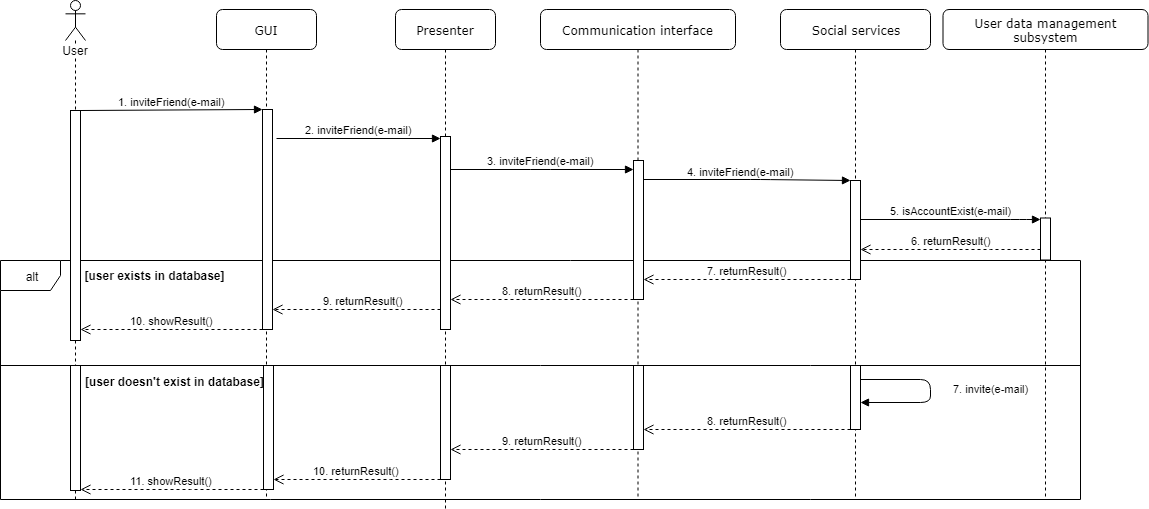
\includegraphics[width=\linewidth]{inviteFriend}
\caption{Zapraszanie użytkownika do skorzystania z aplikacji.}
\label{fig:inviteFriend}
\end{figure}
\FloatBarrier
\subsubsection{Dodawanie znajomego}

\noindent Warunki początkowe:
\begin{enumerate}
  \item Użytkownik jest zalogowany.
  \item Aplikacja ma dostęp do internetu.
  \item Użytkownik wybrał z menu opcję "Znajomi".
\end{enumerate}
\par
\noindent\newline
Warunki końcowe:
\begin{enumerate}
  \item Użytkownik otrzymał informację o rezultacie.
  \item Drugi użytkownik otrzymał informację zaproszenie.
\end{enumerate}

\noindent\newline
\begin{figure}[h]
\centering
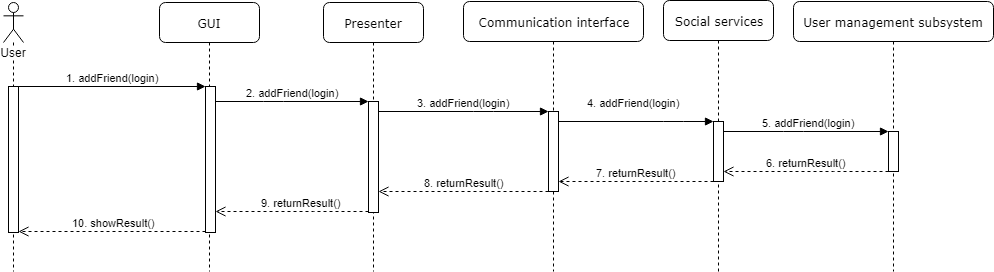
\includegraphics[width=\linewidth]{addFriend}
\caption{Dodanie użytkownika do znajomych.}
\label{fig:addFriend}
\end{figure}
\FloatBarrier
\subsubsection{Udostępnienie podróży}

\noindent Warunki początkowe:
\begin{enumerate}
  \item Użytkownik jest zalogowany.
  \item Aplikacja ma dostęp do internetu.
  \item Użytkownik wybrał podróż do udostępnienia.
  \item Użytkownik docelowy jest znajomym użytkownika udostępniającego.
\end{enumerate}
\par
\noindent\newline
Warunki końcowe:
\begin{enumerate}
  \item Użytkownik otrzymał informację o rezultacie.
  \item Drugi użytkownik otrzymał informację o udostępnionej podróży.
\end{enumerate}

\noindent\newline
\begin{figure}[h]
\centering
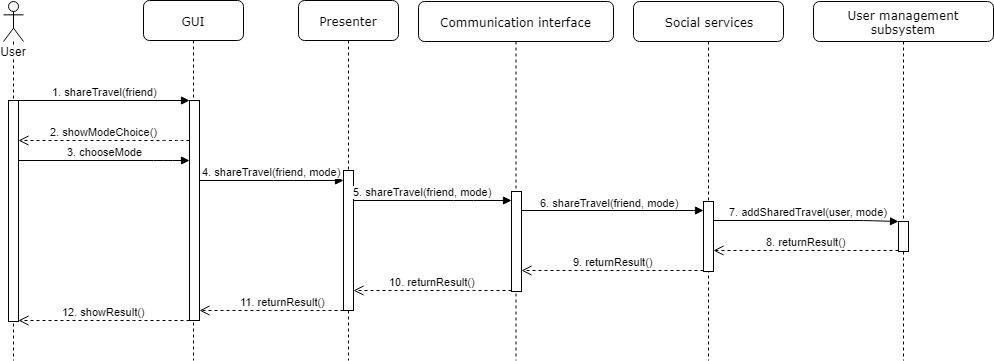
\includegraphics[width=\linewidth]{shareTravel}
\caption{Udostępnienie podróży.}
\label{fig:shareTravel}
\end{figure}

\subsection{Interakcje serwera z aplikacją w czasie trwania podróży (Dorota Tomczak)}
\par Martyna wraz z koleżanką odbywają zaplanowaną poprzez aplikację podróż. W drodze do jednej z atrakcji aplikacja powiadamia Martynę o interesującym obiekcie znajdującym się niedaleko miejsca, w którym przebywają. Dziewczyny ruszają do wskazanej lokalizacji. Tracą poczucie czasu, więc aplikacja informuje je, że jeśli się nie pośpieszą, nie zdążą dojść do następnego punktu planu dnia przed jego zamknięciem (rys.~\ref{fig:whileTravelling}).

\noindent\newline Warunki początkowe:
\begin{enumerate}
  \item Użytkownik jest zalogowany.
  \item Aplikacja ma dostęp do internetu.
  \item Aplikacja ma dostęp do lokalizacji użytkownika.
  \item Użytkownik nie zablokował powiadomień od aplikacji.
  \item Użytkownik utworzył plan podróży i jest w określonym miejscu i czasie.
\end{enumerate}
\par
\noindent\newline
Warunki końcowe:
\begin{enumerate}
  \item Użytkownik otrzymał odpowiednie powiadomienie.
\end{enumerate}

\noindent\newline
\begin{figure}[h]
\centering
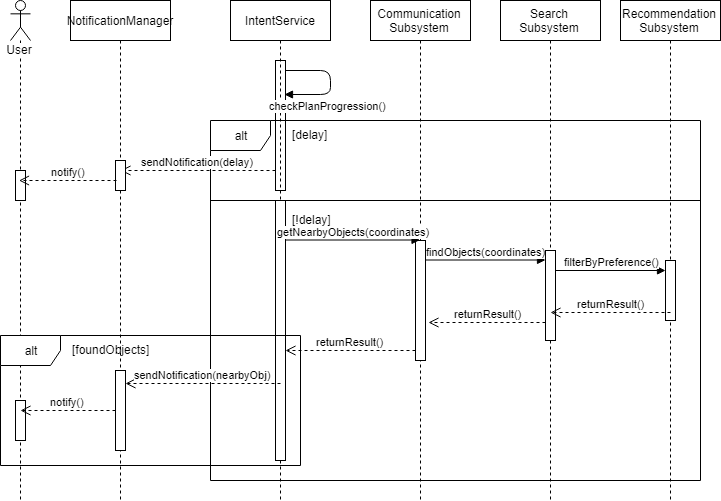
\includegraphics[width=\linewidth]{whileTravelling}
\caption{Otrzymywanie powiadomień podczas trwania podróży.}
\label{fig:whileTravelling}
\end{figure}
\FloatBarrier

\chapter{Decyzje projektowe}

\section{Wybór języka Kotlin (Dorota Tomczak)}
\par Przed rozpoczęciem prac implementacyjnych nad projektem należało podjąć decyzję, co do wyboru języka programowania. W przypadku aplikacji mobilnej na system Android, przy założeniu że miałaby to być aplikacja natywna, wybór ten ograniczał się do dwóch opcji – Java lub Kotlin. Ostatecznie zdecydowano o napisaniu aplikacji w Kotlinie, głównie ze względu na fakt, że 7 maja 2019 firma Google na konferencji Google I/O 2019 ogłosiła, że ten język jest obecnie preferowanym językiem do tworzenia aplikacji mobilnych na Androida\cite{Google I/O 2019}. Aby ułatwić jednoczesną pracę nad aplikacją serwerową podjęto decyzję o wykorzystaniu języka Kotlin również i w tym projekcie.
\par Podczas pracy nad projektem oraz z perspektywy czasu po zakończeniu działań implementacyjnych, jednomyślnie stwierdzono, że wybór Kotlina był słuszny. Język ten zapewnia wiele przydatnych udogodnień i ulepszeń w stosunku do języka Java, które wpływają na jakość kodu i satysfakcję z pracy nad nim. Jedną z jego niezaprzeczalnych zalet jest minimalizacja tzw. kodu boilerplate, co przejawia się między innymi w takich jego cechach jak: 

\begin{itemize}
\item utworzenie klasy typu Singleton jest jednoznaczne z dodaniem klasy oznaczonej słowem kluczowym \textit{object},
\item klasy oznaczone słowem kluczowym \textit{data} służące głównie jako obiekty DTO (obiekty wykorzystywane do przesyłania danych), do których to kompilator sam generuje konstruktory oraz metody dostępu do wszystkich pól,
\item wyrażenia lambda, czyli w uproszczeniu funkcje anonimowe.
\end{itemize}

\begin{figure}[h]
\centering
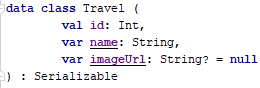
\includegraphics[width=0.7\textwidth]{dtoKotlin}
\caption{Klasa DTO w Kotlinie - 5 linii kodu.}
\label{fig:dtoKotlin}
\end{figure}
\FloatBarrier

\section{Narzędzia (Magdalena Solecka)}
\subsection{Github}
\par W celu łatwego zarządzania projektem wykorzystano System kontroli wersji \textit{Github}. Repozytorium zawierało trzy foldery: App (zawierający implementację aplikacji mobilnej), ServerApp (zawierający implementację serwera REST) oraz Documents (zawierający dokumentację projektu). Backlog produktu utworzono w postaci zadań (ang. issues) również na tej samej platformie.  Jako model pracy wybrano \textit{Gitflow}, a jako schemat nazewnictwa gałęzi funkcjonalności (ang. feature branches): \{nr\_zadania\}-skrócona-nazwa-zadania. Również w nazewnictwie zapisów zmian (ang. commits) zdecydowano się na skorzystanie ze wzoru: \#\{nr\_zadania\}: opis wprowadzonych zmian, w celu śledzenia postępów nad danym zadaniem.

\subsection{Android Studio i Intellij IDEA}
\par Środowiskiem programistycznym wykorzystywanym podczas implementacji zostały wybrane \textit{Android Studio} dla wytwarzania aplikacji mobilnej i \textit{Intellij IDEA} dla serwera. Są to narzędzia kompatybilne z systemem \textit{Git} co znacznie ułatwiło rozwiązywanie konfliktów podczas pobierania najnowszych zmian ze zdalnego repozytorium. Usprawniło również proces zapisu zmian. Konfiguracje systemów członków zespołu wymagały m.in. wykorzystania różnych portów oraz adresów IP. Praca z systemem \textit{Git} poprzez jeden z programów zamiast konsolę umożliwiała odznaczenie konkretnych linii kodu, więc przy każdym zapisie nie trzeba było ich zmieniać.

\subsection{Heroku}
\par Dla celów testowych oraz prezentacji aplikacji zdecydowano się na wdrożenie projektu na zdalny serwer. Skorzystano z darmowej oferty \textit{Heroku}. Skonfigurowano połączenie pomiędzy repozytorium na platformie \textit{Github} a instancją serwerową na platformie \textit{Heroku} tak, aby po jakiekolwiek zmianie na gałęzi develop następowało automatyczne wdrożenie. W celu poprawnej kompilacji projektu na platformie dodano pakiety: https://github.com/timanovsky/subdir-heroku-buildpack (kompilacja projektu znajdującego się w podkatalogu repozytorium) i heroku/gradle (obsługa Gradle).

\chapter{Aplikacja mobilna}

\section{Projekt i implementacja oparte na wzorcu MVP (Dorota Tomczak)}
\par Pracę nad aplikacją mobilną rozpoczęto od stworzenia bazowego projektu składającego się z kilku pustych widoków, do których to następnie można było dodawać kolejne funkcjonalności. W celu zachowania najlepszych praktyk programistycznych zdecydowano się na oparciu projektu o wzorzec architektoniczny MVP (ang. model-view-presenter). Jest to wzorzec szczególnie nadający się do implementacji w aplikacjach mobilnych na systemy Android ze względu na aktywności (ang. activity), które pełnią funkcję środkowej warstwy – widoku (ang. view). W implementacji wzorca w tym projekcie widok jest pasywny (ang. passive view) tzn. widok powinien odpowiadać jedynie za wyświetlanie interfejsu i użycie bibliotek związanych z Androidem. Cała logika aplikacji ma być zawarta w prezenterze (ang. presenter), który pełni funkcję kontrolera.

\par Zastosowanie wzorca MVP pozwoliło na zachowanie porządku w strukturze projektu i przejrzysty podział na warstwy. Do każdej aktywności, czyli nowego ekranu w aplikacji, utworzono interfejs zwany kontraktem (ang. contract) zawierający opis interakcji jakie mogą zajść pomiędzy prezenterem a widokiem, a w szczególnych przypadkach również między prezenterem a adapterem, który odpowiada za wyświetlanie listy obiektów. Klasy aktywności i prezentera implementują interfejsy zawarte w kontrakcie, prezenter jest wstrzykiwany do widoku, a referencja widoku jest przekazywana do prezentera w konstruktorze.

\begin{figure}[h]
\centering
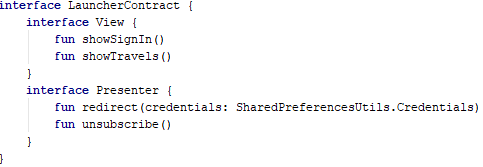
\includegraphics[width=\linewidth]{launcherContract}
\caption{Prosty kontrakt widoku odpowiadający za przekierowanie do widoku logowania lub listy podróży.}
\label{fig:launcherContract}
\end{figure}
\FloatBarrier

\par Do wstrzykiwania zależności, w tym prezenterów do aktywności, wykorzystano popularny framework \textit{Dagger 2}\cite{Dagger 2}, co ostatecznie okazało się być nie najlepszym wyborem – należało dodać dwie dodatkowe klasy do każdej aktywności, co przy dużej ich liczbie wygenerowało wiele plików o bardzo podobnej strukturze. Ponadto niemalże jedynymi wstrzykiwanymi obiektami były obiekty klas prezenterów. 

\section{Komunikacja z aplikacją serwerową (Anna Malizjusz)}
\par Aplikacja mobilna musi komunikować się z RESTowym API udostępnianym przez serwer. W tym celu wykorzystano klienta o nazwie Retrofit 2 \cite{Retrofit library}. Dzięki niemu w łatwy sposób można zaimplementować interfejs odpowiedzialny za wysyłanie zapytań i odbieranie odpowiedzi.

\par Napisano kilka klas, aby umożliwić prostą komunikację w aplikacji. Interfejs \textit{ServerApi} zawierał zbiór metod z odpowiednimi adnotacjami @PUT, @POST, @GET, @DELETE i nazwami punktów końcowych. Metody nie wymagały implementacji przez programistów, ponieważ ich obsługa należała do odpowiedzialności klienta Retrofit 2.

\begin{figure}[h]
\centering
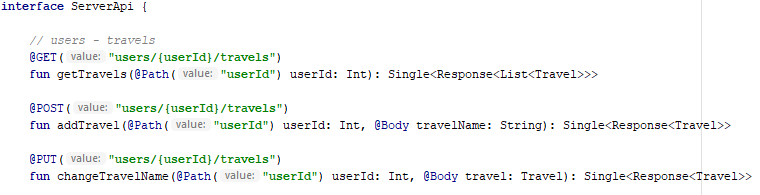
\includegraphics[width=\linewidth]{serverApi}
\caption{Przykładowa zawartość interfejsu używanego przez Retrofit 2.}
\label{fig:tokenPayload}
\end{figure}
\FloatBarrier

\par Dodatkowo zaimplementowano klasę pomocniczą konfigurującą klienta. Udostępniała ona zmienną (ang. property), która była przygotowanym interfejsem do komunikacji. Ustawiono w niej adres serwera REST, a także konwertery przeprowadzające serializację obiektów do formatu JSON oraz deserializację z otrzymanego ciągu znaków w formacie JSON do obiektu będącego instancją danej klasy. Skorzystano z klasy \textit{GsonConverter}, która jest oferowana przez Retrofit API. Wykorzystano wzorzec projektowy interceptor implementując klasę \textit{AuthTokenInterceptor}, którego rolą było dodanie do każdego zapytania nagłówka (ang. header) z lokalnie zapisanym tokenem identyfikującym użytkownika. Interceptor aplikacji jest wywoływany zawsze i tylko jeden raz, nie wpływają na to przekierowania ani ponawianie zapytań. Aby zintegrować interfejs używanego klienta z interceptorem, należało dodać dodatkowego klienta - \textit{OkHttpClient}\cite{OkHttpClient}. Pochodzi z biblioteki OkHTTP, którą również można było wykorzystać do komunikacji aplikacji mobilnej z serwerem, jednak postawiono wybrać Retrofit 2 z uwagi na mniejszy poziom skomplikowania oferowanego API.

\par Rezultatem każdego zapytania jest struktura \textit{Single<Response<T> >}, gdzie T jest oczekiwanym typem zwracanego obiektu. Obiekt \textit{Single} informuje o tym, że jest spodziewana pojedyncza odpowiedź. \textit{Response} jest strukturą zdefiniowaną w projekcie inżynierskim. Zawiera kod odpowiedzi opisywany szerzej przy sposobie implementacji błędów, a także także pole \textit{data} z przesłanymi przez serwer danymi.


\section{Logika rejestracji i logowania (Anna Malizjusz)}
\par Rejestracja użytkownika polega na podaniu trzech informacji: adresu email oraz dwukrotnym podaniu hasła. Każde z tych pól jest walidowane. Adres e-mail powinien mieć formę xxx@yyy.zzz, gdzie xxx, yyy i zzz są dowolnymi ciągami znaków. Hasło nie powinno być trywialne. Musi zawierać co najmniej jedną cyfrę, jedną wielką i jedną małą literę, a także mieć przynajmniej 8 znaków długości. Poprawność walidacji została sprawdzona testami jednostkowymi.

\begin{figure}[h]
\centering
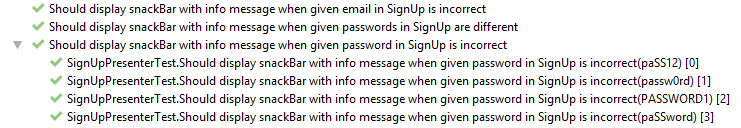
\includegraphics[width=\linewidth]{registerUnitTestResult}
\caption{Testy jednostkowe sprawdzające poprawność sposobu walidacji formularza rejestracji}
\label{fig:tokenPayload}
\end{figure}
\FloatBarrier


\section{Wyszukiwanie atrakcji turystycznych i zakwaterowania (Anna Malizjusz)}
\par Dodanie konkretnego miejsca do planu dnia jest możliwe po jego wyszukaniu. W tym celu stworzono ekran umożliwiający wybranie obiektu z mapy. Na wyświetlanym obszarze są widoczne pinezki odpowiadające obiektom w podanej okolicy.

\par Głównym komponentem widoku wyszukiwania jest \textit{SearchView}\cite{SearchView}. Dzięki temu na ekranie widać pole, w które można wpisać nazwę lub początek nazwy miasta i wybrać je z listy. Mapa automatycznie przeniesie się do wskazanego miejsca. Implementacja mechanizmu podpowiedzi znajduje się w klasie \textit{CitySuggestionProvider}, dziedziczącej po \textit{ContentProvider}\cite{ContentProvider}. Kluczowym było nadpisanie metody \textit{query(Uri, String[], Bundle, CancellationSignal)}, która zwracała wynik do widoku. Używając interfejsu komunikacji z serwerem aplikacja pobierała listę proponowanych miast, a \textit{CitySuggestionProvider} zwracał je w formie kursorów.

\par Po wybraniu pinezki jednego z wyświetlanych obiektów na ekranie pojawia się nazwa miejsca, a także możliwość pokazania jego szczegółów. Zostało to osiągnięte dzięki użytemu układowi o nazwie \textit{SlidingUpPanelLayout}\cite{SlidingUpPanelLayout}. Pozwala on na rozwinięcie i późniejsze ukrycie widocznego na dole obszaru ze szczegółowymi informacjami. Te same dane są w późniejszym etapie dostępne po wybraniu elementu z planu dnia. Z tego powodu postanowiono wyodrębnić układ pól z informacjami, zdefiniować go w osobnym pliku i wykorzystać go zarówno w widoku wyszukiwania, jak i widoku detali obiektu.

\par Uwzględniono szczególny przypadek, jakim jest wyszukanie zakwaterowania. Jeżeli aplikacja wykryje, że dany obiekt jest miejscem noclegu, zaproponuje dodatkowo dodanie daty wykwaterowania. Końcowym efektem będzie pojawienie się dwóch elementów w planach dni. Pierwszy z nich jest podpisany jako zakwaterowanie (ang. check in), a drugi jako wykwaterowanie (ang. check out). Wystawienie oceny jest możliwe tylko dla elementu reprezentującego drugie z tych wydarzeń.


\section{Tworzenie planów podróży (Dorota Tomczak)}
\par Tworzenie planów podróży jest kluczową funkcją aplikacji. Stworzenie takiego planu jest możliwe, gdy użytkownik ma przypisaną do swojego konta dowolną podróż. Dodawanie do niej kolejnego elementu planu zostało zrealizowane poprzez prosty formularz, który zawiera:
\begin{itemize}
\item rozwijaną listę z kategoriami miejsc odpowiadającą wybranym kategoriom z \textit{Here API}\cite{Here},
\item pole z nazwą miejsca, które po dotknięciu przekierowuje do ekranu wyszukiwania, a po wybraniu obiektu wypełnia się automatycznie,
\item pola od dnia i od godziny, po których dotknięciu otwierają się dialogi odpowiednio z kalendarzem i zegarem,
\item pola analogiczne do dwóch powyższych, jeśli wybrano kategorię Zakwaterowanie, oznaczające dzień i godzinę wykwaterowania,
\item pole z adresem, które wypełnia się automatycznie po wyszukaniu obiektu,
\item pole na notatki, które są potem możliwe do edycji.
\end{itemize}

\par Po zatwierdzeniu formularza zostaje on poddany walidacji – wszystkie pola oprócz notatek muszą być wypełnione, a dla kategorii \textit{Zakwaterowanie} (ang. \textit{Accommodation}) czas zakwaterowania nie może być przed czasem wykwaterowania. Jeśli formularz pomyślnie przejdzie próbę walidacji, nowy element planu podróży zostaje utworzony.
Elementy planu dnia wyświetlają się w formie chronologicznej listy rozdzielonej separatorami z datami. Do implementacji tego rozwiązania posłużył adapter, który na podstawie typu elementu określa jaki układ xml (ang. layout xml) wyświetlić – czy ten dla elementu planu czy daty. Aby oba typy mogły być używane przez adapter, muszą dziedziczyć po wspólnym interfejsie, którym jest \textit{DayPlanItem} z jedną metodą, która zwraca typ obiektu.
\par Jednak zanim nowy element planu dnia może zostać przekazany do adaptera i wyświetlony na ekranie jest najpierw dodawany do kolekcji typu \textit{TreeSet}, która sortuje znajdujące się w niej elementy po wyniku zwracanym przez metodę \textit{compareTo(other: PlanElement): Int}, zaimplementowaną w klasie dodawanych elementów. Następnie tworzona jest lista składająca się z separatorów oraz wspomnianych elementów – po sprawdzeniu pola \textit{fromDate} elementu następuje decyzja, czy rozdzielić elementy nowym separatorem z dniem czy nie. Tak przygotowana lista trafia do adaptera i efektem jest widok posortowanych chronologicznie elementów planów dni w podróży.


\section{Implementacja skanowania dokumentów z użyciem OpenCV (Dorota Tomczak)}
\par Aplikacja umożliwia zrobienie zdjęcia, wybranie czworokątnego obszaru oraz takie przycięcie i modyfikację kolorów fotografii, aby uzyskać efekt skanu. W początkowych założeniach zakładano skorzystanie z gotowej biblioteki, która poza wymienionymi wyżej funkcjonalnościami dokonywałaby automatycznej detekcji krawędzi, jednak ze względu na brak darmowych i dostosowanych do potrzeb rozwiązań zdecydowano stworzyć skaner od podstaw bazując na projekcie open-source \textit{SimpleDocumentScanner-Android}\cite{SimpleDocumentScanner-Android}.

\par Wykonanie fotografii jest możliwe jeśli użytkownik nadał aplikacji odpowiednie uprawnienia. Są one weryfikowane przy każdej próbie dodania skanu. Jeśli aplikacja została do tego uprawniona, tworzony jest plik tymczasowy w pamięci urządzenia, a następnie otwierany jest widok kamery za pomocą intencji (ang. intent) utworzonej poprzez podanie do konstruktora nazwy odpowiedniej akcji. Zdjęcie wykonane przez użytkownika jest zapisywane w utworzonym wcześniej pliku tymczasowym a jego ścieżka przekazywana do aktywności (ang. activity) skanera, aby umożliwić w niej jego wyświetlenie i modyfikację.

\par W celu zaimplementowania możliwości wyboru obszaru zdjęcia poprzez gesty użytkownika dodano specjalną klasę dziedziczącą po \textit{ImageView}\cite{ImageView}. Taka klasa mogła zostać następnie dodana do układu xml skanera, a zaimplementowane w niej metody pozwoliły na rysowanie i przeciąganie czterech linii złączonych końcami i tworzących czworokąt. Końce czworokąta są reprezentowane przez cztery zmienne typu \textit{PointF} zawierające informacje o ich położeniu na ekranie urządzenia. Po każdym wykryciu gestu przeciągnięcia linii łączącej punkty, obliczane jest ich nowe położenie, a następnie ponownie złączane są linią. Gdy użytkownik zatwierdzi zaznaczony obszar punkty transformowane są z ich współrzędnych na urządzeniu na współrzędne na zdjęciu.

\par Kolejnym etapem jest uzyskanie efektu zeskanowanego dokumentu. Aby móc to osiągnąć zastosowano bibliotekę \textit{OpenCV}\cite{OpenCV}, której pliki źródłowe musiały zostać dołączone do projektu aplikacji w postaci modułu. Aby ograniczyć rozmiar aplikacji wynikowej, który znacznie wzrósł po dodaniu biblioteki, usunięto jej klasy, które nie były potrzebne do realizacji funkcjonalności. Najważniejszymi operacjami, które dostarczyła OpenCV jest transformacja perspektywiczna (ang. perspective transform), która w ogólności zajmuje się przekształceniem trójwymiarowego świata do dwuwymiarowego obrazka, oraz progowanie obrazu (ang. thresholding), czyli metoda segmentacji obrazu pozwalająca uzyskać obraz binarny z obrazu kolorowego. Otrzymany skan po zastosowaniu tych dwóch operacji i innych pomocniczych może być przez użytkownika zachowany lub odrzucony. W tym pierwszym przypadku zostaje on przesłany na serwer.

\begin{figure}[h]
\begin{subfigure}{0.5\textwidth}
\centering
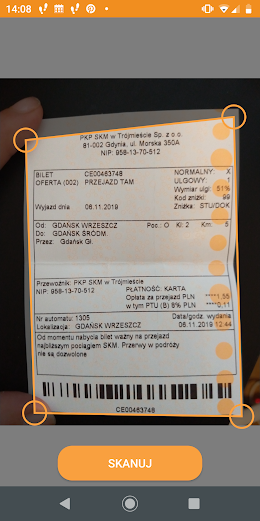
\includegraphics[width=0.9\linewidth, width=5cm]{scan1}
\caption{Zaznaczanie obszaru do skanowania.}
\label{fig:scan1}
\end{subfigure}
\begin{subfigure}{0.5\textwidth}
\centering
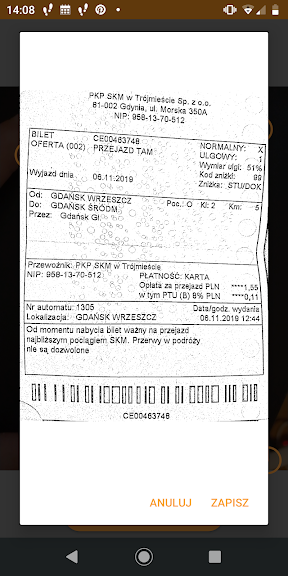
\includegraphics[width=0.9\linewidth, width=5cm]{scan2}
\caption{Skan wynikowy po transformacjach zdjęcia.}
\label{fig:scan2}
\end{subfigure}
\caption{Skanowane biletu.}
\label{fig:Eimage}
\end{figure}
\FloatBarrier

\section{Obsługa przesyłania i pobierania plików (Dorota Tomczak)}
\par Aby umożliwić użytkownikom korzystanie ze swoich kont na różnych urządzeniach oraz udostępnianie stworzonych przez siebie podróży, wynikła konieczność przesyłania dodanych zdjęć na serwer, zamiast przechowywania ich lokalnie na urządzeniach mobilnych. Zdjęciami w aplikacji mogą być wykonane skany lub fotografie dodane do poszczególnych podróży, a ich przesyłanie odbywa się przy pomocy RESTowego API udostępnianego przez serwer, jak zostało to opisane w podrozdziale 5.2. Zapytania za to odpowiadające są dodatkowo opatrzone adnotacją \textit{@Multipart}, aby umożliwić przesyłanie całych plików w ciele (ang. body) żądania, natomiast pliki przekształcane są na obiekt typu \textit{MultiPartBody.Part}. Gdy plik zostanie odebrany po stronie serwera następuje próba jego zapisu w ustawionym w konfiguracji folderze przez \textit{FileStorageService}, czyli serwis do przechowywania plików. Następnie ścieżka do pliku jest dodawana do bazy wraz z innymi niezbędnymi informacjami umożliwiającymi jego identyfikację.

\par Ładowanie plików w aplikacji zostało zrealizowane dzięki bibliotece \textit{Glide}\cite{Glide}, która pozwala na zwiększenie efektywności tego procesu poprzez automatyczne korzystanie z pamięci podręcznej urządzenia i optymalizację rozmiaru zdjęcia. Znając adres, pod którym znajduje się plik, użycie wspomnianej biblioteki jest bardzo proste, dlatego na większą uwagę zasługuje proces wysyłania fotografii przez serwer. Plik o wskazanej nazwie zostaje załadowany jako obiekt typu \textit{Resource} przez \textit{FileStorageService}, a następnie konstruowana jest odpowiedź serwera, która w ciele zawiera otrzymany zasób. Odpowiedź jest dodatkowo opatrzona nagłówkiem \textit{Content-Disposition}, który zawiera informację o tym, że plik ma zostać potraktowany jako załącznik. 

\section{Dodawanie użytkowników do znajomych oraz wyświetlanie listy znajomych (Karolina Makuch)}

\par W celu umożliwienia użytkownikowi udostępniania planu podróży znajomym dodano do aplikacji funkcjonalność odpowiadającą za wyszukiwanie konkretnych użytkowników. Została ona zrealizowana poprzez  wykorzystanie komponentu \textit{SearchView} (\textit{appcompat.widget.SearchView}) zawierającego pole umożliwiające wpisanie ciągu znaków. Podczas wprowadzania kolejnych liter zostają wyświetlane podpowiedzi w czasie rzeczywistym. Aktualizują się  przy każdej zmianie wyrazu. Uwzględniają one wszystkie adresy mailowe zarejestrowanych w aplikacji użytkowników zaczynających się od podanego ciągu znaków.

\par W tym celu została stworzona klasa implementująca abstrakcyjną klasę \textit{ContentProvider} (\cite{ContentProvider}). Po wysłaniu odpowiedniego zapytania zostaje utworzony \textit{MatrixCursor} zawierający dwie kolumny: identyfikator użytkownika oraz jego adres mailowy. Po otrzymaniu odpowiedzi od serwera dla każdego użytkownika zostaje utworzony wiersz, który następnie jest dodawany do kursora. Wyświetlana jest tylko kolumna zawierająca adres mailowy.

\par Kursor został również wykorzystany w celu umożliwienia dodania wybranego użytkownika do znajomych. Podczas kliknięcia na wybrany wiersz zostaje wywoływana nadpisana metoda \textit{onSuggestionClick} obiektu klasy \textit{SearchManager} (\textit{android.app.SearchManager}). Pobiera ona potrzebne dane wybranej pozycji z tablicy \textit{MatrixCursor’a}.

\par Do eliminacji przypadkowych działań zostało wykorzystane okno dialogowe wymagające potwierdzenia  zamiaru dodania wybranego użytkownika do znajomych. W tym celu została wykorzystana klasa \textit{AlertDialog} (\textit{androidx.appcompat.app.AlertDialog}). Po wyrażeniu zgody  oraz w przypadku poprawnego wykonania metody użytkownik otrzymuje powiadomienie stworzone poprzez wywołanie konstruktora klasy \textit{Snackbar} (\textit{com.google.android.material.snackbar.Snackbar}).

\par W tym samym oknie pod polem do wyszukiwania znajduje się lista znajomych użytkownika. Została ona dodana jako liniowa warstwa (ang. \textit{LinearLayout}) umożliwiająca odświeżanie widoku poprzez szybkie przesunięcie palcem po ekranie (ang. \textit{SwipeRefreshLayout}). Implementuje ona tryb usuwania.

\par Powiązanie dwóch użytkowników poprzez oznaczenie ich jako znajomych zostało zrealizowane poprzez dołączenie do bazy danych osobnej tabeli przechowującej potrzebne informacje. Dodawanie jest jednostronne. Znajomy danego użytkownika nie jest zobowiązany do posiadania go na swojej liście znajomych.

\par Po stronie serwera zostały dodane pliki umożliwiające komunikację z wspomnianą powyżej tabelą oraz wykonywaniu potrzebnych zapytań. Oprócz bazowych, niezbędnych do komunikacji zostało również zaimplementowane w jednym zapytanie zwracające wszystkie adresy mailowe nieznajomych użytkowników zawierających wpisany ciąg znaków.

\section{Udostępnianie podróży znajomym (Karolina Makuch)}

\par  Udostępnianie podróży jest możliwe po dodaniu użytkownika do listy znajomych. W momencie wybrania ikony udostępnienia pojawia się okno dialogowe (\textit{androidx.fragment.app.DialogFragment}) zawierające znajomych użytkownika w formie  listy wyboru (ang. \textit{Checkbox}) nie mających dostępu do danego planu podróży. Podczas implementacji została nadpisana metoda \textit{setMultiChoiceItems} w celu umożliwienia udostępnienia planu wielu znajomym podczas jednej czynności.
\par  Po wybraniu osób, zatwierdzeniu decyzji oraz poprawnym wykonaniu metody użytkownik otrzymuje powiadomienie stworzone poprzez wywołanie konstruktora klasy \textit{Snackbar}
(\textit{com.google.android.material.snackbar.Snackbar}). Odpowiednie powiadomienie zostaje również wyświetlone w sytuacji niewybrania ani jednego znajomego oraz potwierdzeniu wykonania czynności.
\par  Każdy użytkownik mający dostęp do podróży posiada prawa do edycji jej planu. Podczas wykonywania czynności udostępniania wybranemu znajomemu zostaje przypisana dana podróż poprzez dodanie powiązania w odpowiedniej tabeli.

\begin{figure}[h]
\centering
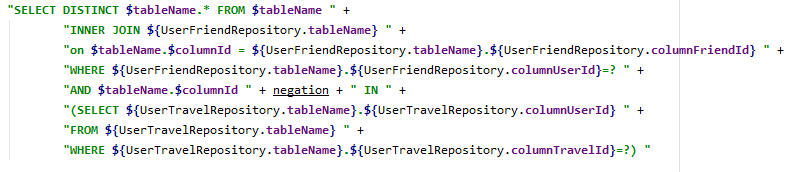
\includegraphics[width=\linewidth]{getFriendsBySharedTravel}
\caption{Zapytanie zwracające listę adresów mailowych znajomych danego użytkownika nieposiadających dostępu do wybranej podróży}
\label{fig:getFriendsBySharedTravel}
\end{figure}
\FloatBarrier

\section{Udostępnianie planu dnia w medium społecznościowym (Karolina Makuch)}
\par  Po dłuższym przytrzymaniu poszczególnego elementu planu pojawia się „dymek"  (\textit{android.widget.PopupMenu}) zawierający trzy czynności do wyboru. Jedną z nich jest możliwość udostępnienia wybranego punktu w medium społecznościowym. Postanowiono wybrać jedno z najpopularniejszych – \textit{Facebooka}. W tym celu wykorzystano akcję wysyłającą (ang. \textit{ACTION.SEND}) za pomocą intencji (\textit{android.content.Intent}).
\par  W przypadku znalezienia aplikacji Facebook na telefonie użytkownika, zostanie on automatycznie przekierowany do publikowania posta na własnej „tablicy”. Domyślną treścią jest link do map HERE \cite{mobileHere} z wyszukanym miejscem z elementu planu dnia. W celu pobrania właściwego odnośnika  zostało zaimplementowane odczytywanie wartości parametru widoku (ang. \textit{view}) znajdującego się w odpowiedzi w formacie JSON (z wykorzystaniem \textit{com.google.gson.JsonParser}). Odsyłacz do wyników zapytania został pobrany z bazy danych. Z racji niemożliwości wykonania analizy (ang. \textit{parse}) wyniku zapytania w głównym wątku aplikacji utworzono osobny wątek.
\par Początkowo planowano inną domyślną treść. Miała ona zawierać najważniejsze informacje na temat wybranego elementu planu. Niestety zarówno wbudowany w Androidzie moduł  udostępniania, a także \textit{API Facebooka} nie udostępnia tej możliwości.  Problem ten został zgłoszony ponad 7 lat temu, lecz nie został rozwiązany\cite{FacebookBug}. Pola \textit{"EXTRA SUBJECT"} oraz \textit{"EXTRA TEXT"} są pomijane w momencie próby udostępniania domyślnej zawartości w aplikacji Facebook. Z racji możliwości załączania zdjęć, linków oraz plików multimedialnych (np. wideo) rozważane było zamienienie tekstu na plik obrazu oraz dodanie go do akcji. Brane również pod uwagę było przeniesienie domyślnej wiadomości do schowka oraz wyświetlenie komunikatu informującego użytkownika z prośbą o wklejenie wiadomości.
\par Jednakże stwierdzono, że takich akcji nie powinno się wymagać od użytkownika. Ostatecznie postanowiono, że najlepszym rozwiązaniem będzie zdecydowanie się na wspomniany wcześniej odsyłacz do wyszukanego miejsca z mapy HERE \cite{mobileHere}. Dzięki czemu treść posta zostanie utworzona przez użytkownika umożliwiając mu zachowanie własnego charakteru pisania.

\section{Manualna realizacja planu (Karolina Makuch)}
\par  Kolejną akcją dostępną w „dymku” pojawiającym się po przytrzymaniu poszczególnego elementu jest manualna realizacja planu dnia. Początkowa treść akcji dla nowo powstałego nieukończonego jeszcze elementu planu dnia brzmi \textit{„Oznacz jako ukończony”} (ang. \textit{„Mark as completed”}). W przypadku oznaczenia części składowej planu jako zrealizowany tekst automatycznie zmienia się na \textit{„Oznacz jako nieukończony”} (ang. \textit{„Mark as incompleted”}) oraz zwiększa się stopień przeźroczystości odpowiedniego elementu listy. Postanowiono oznaczać zrealizowane plany poprzez wygaszenie kolorów elementów danego planu zmniejszając wartość kanału \textit{alfa} (ang. \textit{Alpha}).
 \par Zdecydowano się umożliwić użytkownikowi cofnięcie wprowadzonych zmian w przypadku wykonania niechcianego kliknięcia, świadomie rezygnując z wymagającego potwierdzenia okna dialogowego. Stwierdzono duże prawdopodobieństwo wykonywania tej akcji w pośpiechu. Dodatkowe kliknięcie wydłużyłoby czas wykonywania akcji oraz mogłoby to irytować użytkownika.
\par  Oznaczenie planu jako wykonany zostało umożliwione dzięki dodaniu odpowiedniej kolumny do tabeli zawierającej plany dni. Dzięki temu każdy użytkownik mający dostęp do podróży ma możliwość wykonania tej czynności i jej efekty są widoczne dla wszystkich uczestników wyprawy.

\section{Tryb usuwania (Magdalena Solecka)}
\par Usuwanie podróży, skanów, elementów planu dnia oraz znajomych jest możliwe przez wybranie z menu kontekstowego, pojawiającego się po przytrzymaniu obiektu, opcji usuń. Powoduje to przejście do trybu usuwania zaimplementowanego z użyciem trybu akcji (ang. Contextual Action Mode) oferowanego przez Android. Na żądanie usunięcia wybranych elementów wysłane do serwera, odpowiada on listą identyfikatorów poprawnie usuniętych  obiektów, które następnie są usuwane z widoku aplikacji. Dzięki temu nie jest konieczne wysyłanie dodatkowego żądania w celu zaktualizowania listy po stronie klienta.

\chapter{Serwer REST}
\section{Implementacja serwera (Anna Malizjusz)}
\par Serwer dla aplikacji mobilnej został zaimplementowany w języku Kotlin. Celem było stworzenie bezstanowego API zgodnego z tzw. RESTful Web Service. Oznacza to, że na serwerze nie jest utrzymywana sesja użytkownika, a każde zapytanie jest niezależne od poprzednich. Każdorazowo należy podać wszystkie niezbędne informacje niezbędne do realizacji żądania, m. in. token, który potwierdza tożsamość użytkownika i uprawnia go do określonych akcji.
\par Wykorzystano framework Spring Boot\cite{Spring documentation}. Jest on oparty na platformie Spring, która dostarcza mechanizmów wstrzykiwania zależności, możliwości użycia wzorca MVC (ang. model-view-controller), a także modułów do implementacji testów jednostkowych. Celem obu frameworków jest ułatwienie implementacji serwera. Jedną z zalet użytego niniejszej pracy frameworka jest prosta konfiguracja, która nie wymaga tworzenia plików w formacie xml. Wynika to z zastosowania reguły \textit{konwencja ponad konfigurację} (ang. convention over configuration). Programista nie musi definiować wszystkich ustawień, jeśli stosuje się do przyjętych konwencji. W przypadku technologii Spring Boot kluczowe są adnotacje nad klasami pełniącymi określone role. 
Konfiguracja serwera zachodzi automatycznie na podstawie zależności, jeśli dodano adnotację "@EnableAutoConfiguration" do klasy uruchamiającej serwer. Framework dostarcza również narzędzi do tworzenia punktów końcowych (ang. endpoints).

\par Skorzystano z mechanizmu wstrzykiwania zależności. Klasy mogą być oznaczone jako komponenty (@Component), serwisy (@Service). Serwis jest szczególnym typem komponentu. Komponenty są zarządzalnymi obiektami w aplikacji oraz mogą być wstrzykiwane do pól odpowiedniego typu, które są oznaczone adnotacją @Autowired. Serwisy to elementy, które należą do logiki biznesowej.
 
\par Definicję punktów końcowych umieszczono w klasach kontrolerów oznaczonych adnotacją "@RestController". Zdefiniowano kilka rodzajów kontrolerów, aby rozdzielić odpowiedzialność za poszczególne zadania:
\begin{itemize}
\item kontroler użytkowników jako \textit{ServerUserController}
\item kontroler podróży jako \textit{ServerTravelController}
\item kontroler odpowiedzialny za skany jako \textit{ServerScanController}
\item kontroler pośredniczący w komunikacji z zewnętrznym API dostarczanym przez firmy Google oraz Here: \textit{ServerHereGoogleApiController}
\item kontroler funkcji rekomendujących: \textit{ServerRecommendationController}
\end{itemize}

\par W każdym z kontrolerów wyróżniono punkty końcowe (ang. endpoints). Zastosowano powszechną konwencję nazewnictwa oraz znaczenie czasowników protokołu HTTP. Przykładowo dodawanie (POST), usuwanie (DELETE), aktualizacja (PUT) oraz odczytanie (GET) podróży obsługiwane w kontrolerze \textit{ServerTravelController} odbywa się w następujący sposób:
\begin{itemize}
\item \textit{@GetMapping("users/{userId}/travels")} zwraca podróże należące do użytkownika o podanym numerze ID;
\item \textit{@PostMapping("users/{userId}/travels")} dodaje podróż podaną w ciele zapytania (ang. body) do podróży użytkownika o podanym numerze ID;
\item \textit{@PutMapping("users/{userId}/travels")} aktualizuje podróże zawarte w ciele zapytania (ang. body);
\item \textit{@DeleteMapping("users/{userId}/travels")} umożliwia usunięcie listy podróży, która została wysłana w ciele zapytania.
\end{itemize}

\par Każde zapytanie powinno zawierać w nagłówku token użytkownika, który jest sprawdzany w celu weryfikacji źródła zapytania. Parametry ścieżki (ang. path parameters) punktów końcowych uszczegóławiają zasób, np. "userId" w powyższym przykładzie. Dodatkowe parametry zapytania (ang. query parameters) i ciało zapytania(ang. body) pozwala na sprecyzowanie żądania.

\section{Obsługa sytuacji wyjątkowych (Dorota Tomczak)}
\par Aplikacja mobilna komunikuje się z serwerem poprzez RESTowe API, jeśli więc po stronie serwera dojdzie do sytuacji wyjątkowej, aplikacja powinna otrzymać wiadomość o tym, co poszło nie tak i odpowiednio ją obsłużyć. W tym celu zdefiniowano kilkanaście własnych wyjątków, czyli klas dziedziczących po klasie java.lang.Exception oraz implementujących własny interfejs ApiException, który zawiera kod błędu wraz z wiadomością opisującą błąd. W celu uniknięcia tworzenia wielu bloków try-catch oraz powielania bloków kodu zaimplementowano globalny moduł obsługi wyjątków, czyli klasę opatrzoną adnotacją \textit{@RestControllerAdvice}, zawierającą dwie metody z adnotacjami \textit{@ExceptionHandler} – jedna służąca do obsługi nowo zdefiniowanych wyjątków, a druga do pozostałych. W obu tych metodach złapany wyjątek jest dodawany do logów serwera, a następnie zwracana jest odpowiedź z odpowiednim kodem błędu. Tak zdefiniowany moduł pozwala na obsługę wszystkich wyjątków występujących na serwerze po dowolnym żądaniu obsłużonym przez każdy z kontrolerów.

\section{Uwierzytelnienie i autoryzacja użytkownika (Anna Malizjusz)}
\par Podstawowy mechanizm uwierzytelnienia i autoryzacji opiera się na standardzie opisanym po raz pierwszy w 2010 roku jako JSON Web Token. Jest on "kompaktowym i bezpiecznym sposobem przesyłania informacji między dwiema stronami" (RFC 7519\cite{JWT}). Użyto biblioteki \textit{io.jsonwebtoken.jjwt}\cite{JWT library}, która dostarcza interfejs do generowania i odczytywania tokenów w przystępny sposób.

\par Uwierzytelnienie użytkownika odbywa się podczas logowania. Serwer porównuje podany adres e-mail oraz zmodyfikowane funkcją mieszającą hasło z danymi zapisanymi w bazie danych. Jeżeli informacje są zgodne, na ich podstawie jest generowany token. JWT pozwala na dodanie twierdzeń (ang. claims) i ustawienie czasu ważności, które zostaną zaszyfrowane przy pomocy algorytmu HS256 i sekretnego klucza. Używane są następujące twierdzenia określające podane cechy tokenu:
\begin{itemize}
\item \textit{iss} - wydawca tokenu (ang. issuer),
\item \textit{sub} - podmiot (ang. subject),
\item \textit{email} - adres e-mail użytkownika,
\item \textit{id} - id użytkownika,
\item \textit{generatedTimestamp} - czas wygenerowania tokenu.
\end{itemize}
\par Przykładowy token zapisany składający się z 3 części XXX.YYY.ZZZ zaprezentowano poniżej:\\eyJhbGciOiJIUzI1NiJ9.eyJzdWIiOiJBY2Nlc3NUb2tlbiIsImdlbmVyYXRlZFRpbWVzdGFtcCI6eyJ5Z\\WFyIjoyMDE5LCJtb250aCI6Ik5PVkVNQkVSIiwibW9udGhWYWx1ZSI6MTEsImRheU9mTW9udG\\
giOjE3LCJjaHJvbm9sb2d5Ijp7ImlkIjoiSVNPIiwiY2FsZW5kYXJUeXBlIjoiaXNvODYwMSJ9LCJkYXl\\
PZldlZWsiOiJTVU5EQVkiLCJsZWFwWWVhciI6ZmFsc2UsImRheU9mWWVhciI6MzIxLCJlcmEiOi\\
JDRSJ9LCJpc3MiOiJUcmF2ZWxBcHBfU2VydmVyIiwiaWQiOjEwLCJleHAiOjE1NzQxMDc4NTksI\\mVtYWlsIjoicXFxMSJ9.vs9PVbgkzxsLpRqxXY0Jaey6fmMXdOLwQW\_dUe9Xxcw

\par Pierwsza część to zakodowany nagłówek, który zawiera algorytm szyfrujący oraz typ tokenu. 
Kolejna jest zawartość, którą tworzą określone przy generacji tokenu twierdzenia. Ostatnia część to podpis. Użyto w nim znanego tylko serwerowi sekretnego klucza, niezbędnego do odszyfrowania otrzymanego od klienta tokenu.
\par Użytkownik aplikacji mobilnej przechowuje swój token i każdorazowo dołącza go do wysyłanych zapytań. Aplikacja serwerowa przy użyciu klucza odczytuje go i weryfikuje otrzymane dane, w szczególności datę ważności tokenu oraz id użytkownika.

\par Rozszyfrowany token jest zapisywany w formacie JSON w postaci, która jest czytelna i zrozumiała dla człowieka. Dzięki użytej bibliotece \textit{io.jsonwebtoken.jjwt} z tokenu w formacie JSON można odczytywać dane jak ze słownika, np.
\textit{Jwts.parser().setSigningKey(SECRET\_KEY).parseClaimsJws(token).body["id"].toString()}, aby odczytać wartość twierdzenia o nazwie "id".

\begin{figure}[h]
\centering
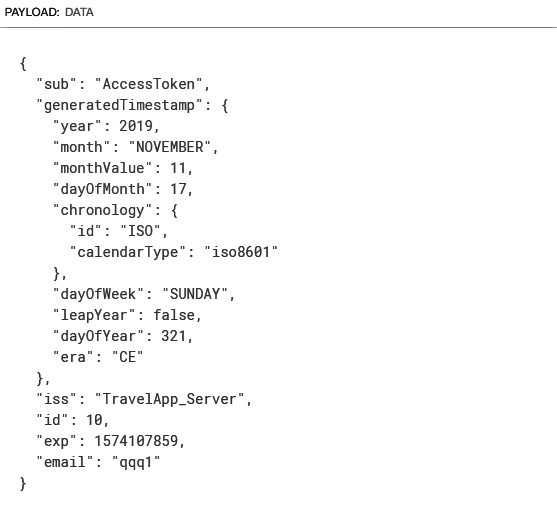
\includegraphics[width=\linewidth]{tokenPayload}
\caption{Rozszyfrowana zawartość podanego powyżej tokenu.}
\label{fig:tokenPayload}
\end{figure}
\FloatBarrier


\section{Komunikacja z zewnętrznym API (Anna Malizjusz)}
\par Potrzeba wyszukiwania infromacji o miejscach na świecie wymusiła korzystanie z zewnętrznych dostawców danych. Po analizie przeprowadzonej na etapie tworzenia specyfikacji wymagań systemowych zdecydowano o użyciu Here API \cite{HereApi}. Próba implementacji rozwiązania zmusiła programistów do skorzystania zarówno z wybranego dostawcy, jak i z początkowo odrzuconego Google API\cite{GoogleApi}, które oferowało dużo bogatszą bazę sposobów transportu.

\par Podstawowym problemem było odczytanie danych. Wynikiem wysłania zapytania do dostawcy informacji był ciąg znaków zawierający znaczą ilość danych nie tylko o temacie zapytania. W przypadku każdego typu żądania przeanalizowano wynik i zdefiniowane wspólną metodę wyszukującą oraz wybierającą niezbędne informacje. Następnie należało je dopasować do potrzeb - nie wszystkie informacje były potrzebne aplikacji. Napisano funkcję zmieniającą ciąg znaków na instancję klasy. Skorzystano z możliwości klasy \textit{JsonParser}\cite{JsonParser} oraz \textit{GsonBuilder}\cite{GsonBuilder}.

\par Należało też uwzględnić sposób zapisanych informacji. Wiele znaków, np. "'" było zakodowanych, aby uniemożliwić wstrzykiwanie złośliwego kodu. W celu rozwiązania tego problemu skorzystano z funkcji \textit{StringEscapeUtils.unescapeHtml3()}\cite{escapeUtils}, która zmieniła formę znaków z kodowej na graficzną.

\section{Wspólne klasy serwera i aplikacji}
\par Podczas implementacji napotkano na problem powtarzających się klas w identycznej formie po stronie aplikacji i serwera. Stwarzało to kłopot przy edycji - obie wersje pliku musiały być zawsze identyczne. Spróbowano rozwiązać to na następujące sposoby.

\subsection{Oddzielny projekt dodany jako moduł (Dorota Tomczak)}
\par Pierwszym pomysłem na wydzielenie wspólnych klas z projektu aplikacji i serwera było utworzenie osobnego projektu, który by te klasy zawierał. Następnie nowy projekt mógłby być dołączony jako moduł do obu projektów, co jednak okazało się być nietrywialnym rozwiązaniem między innymi ze względu na różnice w plikach gradle - plik build.gradle w aplikacji mobilnej został napisany w języku Groovy, natomiast ten na serwerze w Kotlinie. Obie próby stworzenia takiego pliku dla wspólnego modułu w każdym ze wspomnianych języków nie powiodły się. Moduł mógł działać z określonym plikiem gradle tylko dla jednego z projektów jednocześnie. IDE, na którym otwarty był serwer podpowiadało, by usunąć wersję Kotlina w build.gradle, natomiast IDE aplikacji mobilnej podpowiadało wykonanie przeciwnej akcji. Po wielu próbach, ostatecznie porzucono zaproponowany pomysł na stworzenie osobnego projektu ze współdzielonymi klasami.

\subsection{Submoduły w repozytorium (Anna Malizjusz)}
\par Podjęto próbę dodania repozytorium zawierającego tylko wspólne pliki, a następnie wstawienia go do głównego repozytorium jako submoduły. Stworzyło to kolejne problemy w postaci konieczności częstych aktualizacji submodułów.
\par Zrezygnowano z submodułów i wykorzystano symboliczne powiązania.
Git traktował powiązany folder jako istniejący, więc nie powodowało to dodatkowych problemów. Plik zmieniony i zapisany w jednej z lokalizacji był automatycznie odwzorowywany w drugiej. Rozwiązanie to, choć z pozoru skuteczne nie mogło być wykorzystane przez wszystkich członków zespołu ze względu na różnice w systemie operacyjnym. Używane były zarówno komputery z system Windows, Linux oraz MacOS. Ostatecznie próby rozwiązania zarzucono.


\section{Rekomendacja miejsc z wykorzystaniem Collaborative Filtering (Dorota Tomczak)}
\par Po dodaniu elementu planu podróży można wejść w jego szczegóły i dokonać oceny miejsca, które znajduje się w planie. Oceny miejsc w skali od jednego do pięciu są przechowywane wraz z użytkownikami, którzy wystawili daną ocenę w osobnej tabeli bazy danych. Na podstawie tych ocen mogą być następnie obliczane rekomendacje przy użyciu techniki zwanej \textit{Collaborative Filtering}, a w szczególności jej odmianą opartą na użytkowniku (ang. user-based).
\par Do implementacji wspomnianej metody wyznaczania poleceń wykorzystano bibliotekę \textit{Apache Mahout}\cite{Apache Mahout}, która oferuje wiele implementacji algorytmów opartych o uczenie maszynowe. Po wskazaniu źródła danych, czyli w tym przypadku tabeli w bazie, utworzono model danych, który posłużył do wykonania niezbędnych obliczeń. Wyznaczenie polecanych miejsc przebiega w następujący sposób: wyliczane jest podobieństwo między użytkownikami algorytmem współczynnika korelacji Pearsona, algorytm k – najbliższych sąsiadów dla k równego 2 wyznacza najbardziej polecane miejsca, a na koniec na podstawie otrzymanych wyników tworzony jest obiekt klasy \textit{GenericUserBasedRecommender}. Wywołanie metody \textit{recommend} na obiekcie z podanym identyfikatorem użytkownika i liczbą rekomendacji, które ma zwrócić, skutkuje otrzymaniem listy identyfikatorów polecanych miejsc, jeśli zostały jakieś znalezione.
\par Testy przedstawionego rozwiązania aplikacją \textit{Postman}\cite{Postman} wykazały, że zwrócenie odpowiedzi trwa bardzo długo (nawet 20 s), a im większa liczba danych w bazie tym czas oczekiwania się wydłużał. Aby uniknąć konieczności oczekiwania na wynik po stronie aplikacji mobilnej, zdecydowano na prezentację polecanych miejsc w postaci powiadomień, czyli w momencie, gdy serwer jest gotowy na wysłanie rekomendacji wysyła odpowiednie powiadomienie, a do tego czasu użytkownik może dalej swobodnie nawigować po aplikacji.
\par W celu wysyłania powiadomień od serwera do aplikacji mobilnej skorzystano z usługi \textit{Firebase Cloud Messaging}\cite{Firebase}. Serwer po obliczeniu polecanych miejsc buduje wiadomość w postaci mapy, która ma zostać wysłana na urządzenie o określonym unikalnym tokenie. Za wysłanie odpowiada instancja klasy \textit{FirebaseMessaging}. W konsoli usługi można zobaczyć statystyki wysłanych wiadomości, które zawierają między innymi informacje o tym, ile z nich zostało otwartych przez użytkowników. Do odbierania wiadomości po stronie aplikacji mobilnej zaimplementowano serwis, który dzięki temu, że dziedziczy po \textit{FirebaseMessagingService} może reagować na zdarzenia takie jak nadejście wiadomości oraz zmiana tokena.
\par Gdy serwis odbierze wiadomość, odczytuje ją, a następnie tworzy powiadomienie, ustawiając jego parametry takie jak m.in. jego tytuł, priorytet, dźwięk. Powiadomienie jest następnie obsługiwane przez \textit{NotificationManager} i wyświetla się na ekranie urządzenia mobilnego. Użytkownik może powiadomienie od razu usunąć lub otworzyć. W drugim przypadku zostaje on przekierowany do aplikacji mobilnej, gdzie zostaje mu zaprezentowana lista polecanych miejsc wraz z nazwą i adresem.

\section{Dodawanie podróży (Magdalena Solecka)}
\par Podczas dodawania podróży tworzone są rekordy w dwóch tabelach bazy danych: \textit{travel} oraz \textit{app\_user\_travel}. Dodanie tylko jednego z nich powodowałoby zaśmiecanie bazy. W celu zapobiegnięcia takiej sytuacji wykorzystano transakcję. Zmienna autocommit zostaje ustawiona na false, co jest równoznaczne z wymuszeniem manualnego wykonania operacji zapisu (ang. commit). Dodawane są kolejno dwa rekordy. W przypadku błędu zapisu do bazy wykonywana jest operacja cofnięcia operacji (ang. rollback). Jeżeli nie nastąpił żaden błąd wykonywana jest operacja zapisu (ang. commit), a zmiennej autocommit przepisywana jest z powrotem wartość true.

\section{Dostęp do bazy danych (Magdalena Solecka)}
\par Do implementacji połączenia z bazą został wykorzystany PostgreSQL JDBC Driver. Zastosowano wzorzec Singleton, który w języku kotlin implementuje się używając słowa kluczowego \textit{object} zamiast \textit{class}.
\par Zaimplementowano również wzorzec repozytorium (ang. repository pattern). Stworzono bazowy interfejs generyczny IRepository oraz jego implementację - Repository zawierajace operacje typu CRUD. Repozytoria dla poszczególnych modeli DAO dziedziczą po generycznej klasie bazowej Repository. Implementują również własny interfejs z funkcjami wymaganymi dla danej tabeli. Problemem przy wykorzystaniu typu generycznego okazało się tworzenie nowego obiektu, dlatego postanowiono wymusić na programistach implementację dodatkowej funkcji T tworzący ten obiekt dodając ją do interfejsu IRepository. W celu zmniejszenia ilości powtarzającego się kodu wyodrębniono również stałe fragmenty tekstu z zapytań SQL takie jak na przykład \textit{SELECT * FROM tableName } w postaci stałej selectStatement. Stałe zostały dodane do klasy bazowej Repository jako abstrakcyjne. W podobny sposób rozwiązano problem powtarzających się nazw tabel i kolumn. Nie udało się jednak utworzyć stałej abstrakcyjnej, wynikiem prób była pusta wartość w zapytaniach w miejscu gdzie powinna była znaleźć się na przykład nazwa tabeli.
	

\chapter{Baza danych}
\section{Wybór (Magdalena Solecka)}
\par Przy wyborze systemu do zarządzania bazą danych były brane pod uwagę \textit{Neo4j} oraz \textit{PostgreSQL}. Pierwsza z wymienionych wzbudziła zainteresowanie ze względu na planowaną implementację algorytmu rekomendującego Collaborative Filtering. Jej zaletą, jako grafowej bazy danych, byłoby szybkie wydobycie podobieństw pomiędzy użytkownikami na podstawie ocenionych przez nich miejsc. Uznano jednak, że zespół pracował do tej pory z relacyjnymi bazami danych i językiem sql a dłuższe wykonanie algorytmu nie spowoduje problemów z wydajnym działaniem pozostałych funkcjonalności aplikacji, dlatego ostatecznie zdecydowano się na \textit{PostgreSQL} chwalonego za wysoką wydajność, oferującego wsparcie typu BJSON, który mógłby być przydatny przy  przechowywaniu większej ilości informacji o obiektach, a także znajomą zespołowi składnię zapytań. Bazę danych wdrożono w serwisie \textit{ElephantSQL} z instancją \textit{tiny turtle}
 która pozwalała na zapis 20 MB danych, 5 równoległych połączeń z bazą co było w zupełności wystarczające dla środowiska testowego.

\section{Schemat ERD (Magdalena Solecka)}
\par Stworzony przy użyciu narzędzia \textit{ERD Constructor}.

\noindent\newline
\begin{figure}[h]
\centering
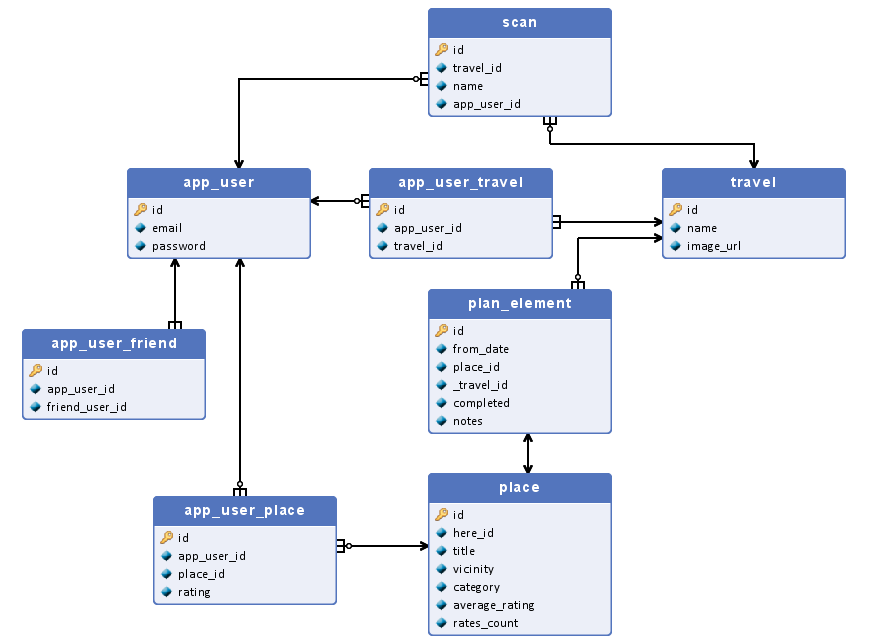
\includegraphics[width=\linewidth]{erd}
\caption{Diagram ERD}
\label{fig:erd}
\end{figure}
\FloatBarrier

\section{Praca z bazą danych (Magdalena Solecka)}
\par Warstwę danych tworzono podejściem \textit{najpierw kod} (ang. code first), głównie z powodu trudności z przewidzeniem, które struktury dostarczane przez zewnętrzne API uda się otrzymać i które informacje są niezbędne, aby znacząco nie zmniejszyć szybkości aplikacji, a o które można zapytać źródło podczas ładowania elementów ekranu. Stwarzało to problemy z kompatybilnością wsteczną podczas rozwijania aplikacji, dodawania nowych kolumn, zmiany typów. Początkowe rozwiązanie wymagało powiadomienia wszystkich programistów w zespole o godzinach, w których baza danych może przestać działać poprawnie, a przed jakąkolwiek dalsza pracą konieczne było ściągnięcie najnowszych zmian z repozytorium \textit{github}. Drugi w kolejności wprowadzonym sposobem było utworzenie tabeli tymczasowej - wykonanie kopii tabeli oraz wprowadzenie zmian w kopii. Podmiany dokonywano przy dołączaniu zmian z gałęzi podrzędnej do gałęzi develop w serwisie \textit{github}. Nadal jednak wymagane było pobranie najnowszej wersji kodu. Z początku wymagało to zaplanowania pracy w ten sposób, aby lokalny kod nadawał się do zapisu (ang. commit) w chwili zmian w bazie, ale problem zakończył się odkryciem funkcji \textit{stash / unstash changes} oferowanej przez gita.

\chapter{Testy}

\section{Testy jednostkowe i instrumentalne aplikacji mobilnej (Dorota Tomczak)}
\par Dla aplikacji mobilnej napisano 23 testy jednostkowe oraz 9 instrumentalnych, które obejmują klasy i metody komponentów służących do logowania, rejestracji oraz przekierowania po starcie aplikacji. Testy jednostkowe, czyli takie które weryfikują poprawność realizacji pojedynczych funkcjonalności aplikacji, zostały zbudowane w oparciu o następujące zależności: \textit{JUnit 4}\cite{JUnit}, \textit{JUnitParams}\cite{JUnitParams} do tworzenia testów parametryzowanych oraz bibliotekę \textit{MockK}\cite{MockK} służącą do tworzenia atrap obiektów (ang. mock object) w języku Kotlin. Testy te służą do weryfikacji działania metod zdefiniowanych w prezenterach, z tego względu przed startem każdego z nich odpowiedni prezenter nie jest atrapą, ale jest inicjalizowany w sposób, który umożliwia jego „szpiegowanie”. Aby zasymulować asynchroniczną komunikację sieciową pomiędzy aplikacją a serwerem, która odbywa się poprzez zastosowanie biblioteki \textit{RxJava}\cite{RxJava}, stworzono klasę pomocniczą \textit{RxImmediateJavaSchedulerRule}, która ustawia wszystkie metody, rozpoczynające nowe wątki, aby korzystały zamiast tego z wątku obecnego.
\par Testy instrumentalne, czyli takie które działają na emulatorze lub na fizycznym urządzeniu mobilnym, zostały zrealizowane dla dwóch aktywności – \textit{SignInActivity} oraz \textit{SignUpActivity} i testują, czy na ekranie wyświetlają się prawidłowe informacje, czy akcje użytkownika wywołują odpowiednie metody oraz czy aplikacja reaguje na nie w odpowiedni sposób. Wykorzystują wiele zależności, w tym między innymi \textit{Espresso}\cite{Espresso} i \textit{MockK-Android}\cite{MockK-Android}. W klasach testowych tworzone są role aktywności (\textit{activityScenarioRole}), na których następnie można wywoływać określone akcje np. wciśnięcie przycisku, czy wpisanie tekstu w polu do tego przeznaczonym. 
\par Wszystkie testy, zarówno instrumentalne jak i jednostkowe zostały podzielone na trzy segmenty:
\begin{itemize}
\item \textit{given} - definicja danych wejściowych oraz symulowanie wywołań metod i tworzenie atrap obiektów,
\item \textit{when} - wywołanie testowanej metody lub wykonanie akcji,
\item \textit{then} - weryfikacja otrzymanych rezultatów po wywołaniu metody lub wykonaniu akcji.
\end{itemize}
Do nazewnictwa testów przyjęto następującą konwencję: co powinno się stać, gdy zostaną spełnione określone warunki. Przykładowo "Should display snackBar with info message when given password in SignUp is incorrect", co w tłumaczeniu oznacza "Powinien się wyświetlić snackBar z komunikatem informacyjnym, gdy hasło podane w SignUp jest nieprawidłowe".

\begin{figure}[h]
\centering
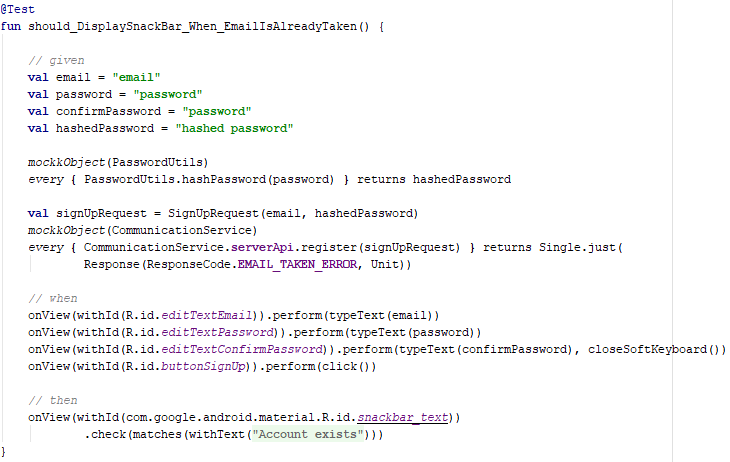
\includegraphics[width=\linewidth]{instrumentationTest}
\caption{Przykładowy test instrumentalny.}
\label{fig:instrumentationTest}
\end{figure}
\FloatBarrier


\chapter{Podręcznik użytkownika (Karolina Makuch)}
\par W celu wytłumaczenia obsługi stworzonej aplikacji oraz zaprezentowaniu jej wizualnej strony przygotowano podręcznik użytkownika. Zawiera on poszczególne etapy wykonywania najważniejszych funkcjonalności.
Aplikacja została zaimplementowana w dwóch wersjach językowych. Dostępny jest język polski oraz angielski.
W trakcie implementacji została podjęta decyzja o zmianie wyglądu aplikacji. Zdecydowano się na weselsze kolory.

\begin{figure}[h]
\centering
\begin{subfigure}{0.3\textwidth}
\centering
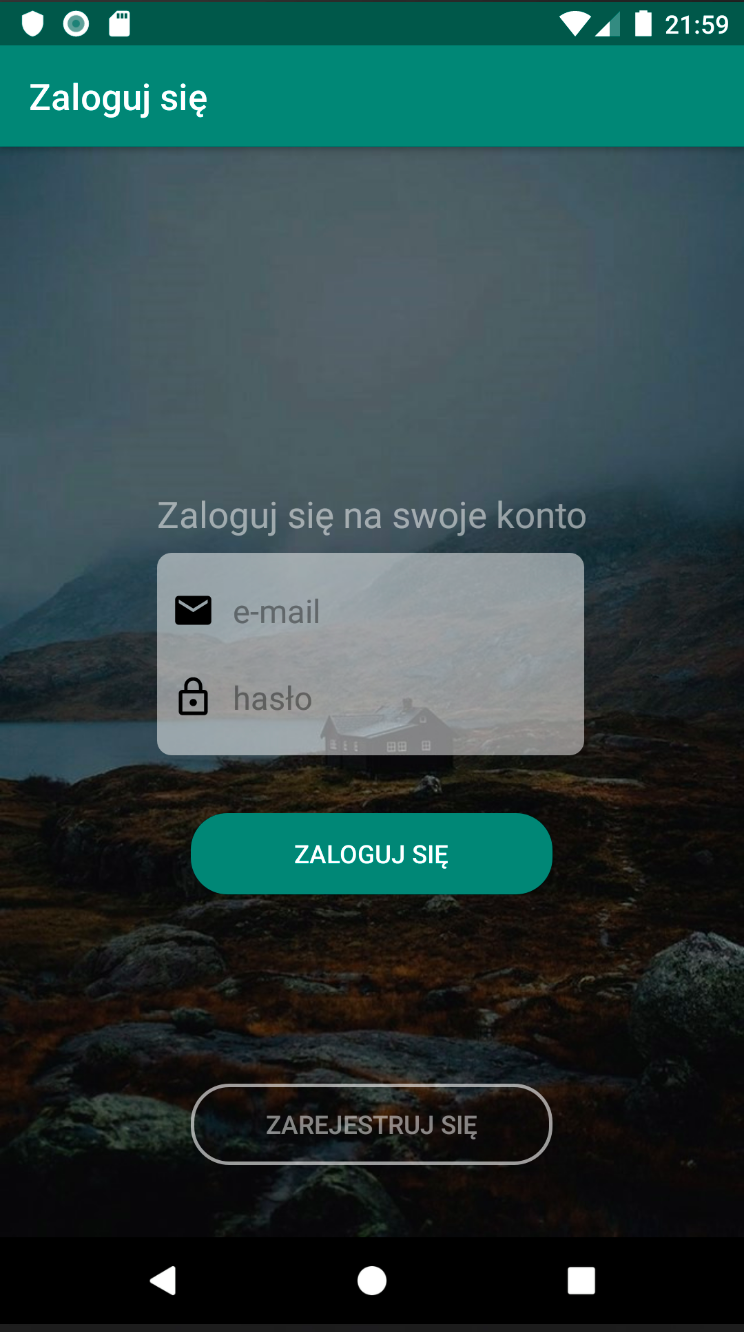
\includegraphics[width=0.8\linewidth, width=5cm]{firstDesign1}
\caption{Widok logowania}
\label{fig:firstDesign1}
\end{subfigure}
\begin{subfigure}{0.3\textwidth}
\centering
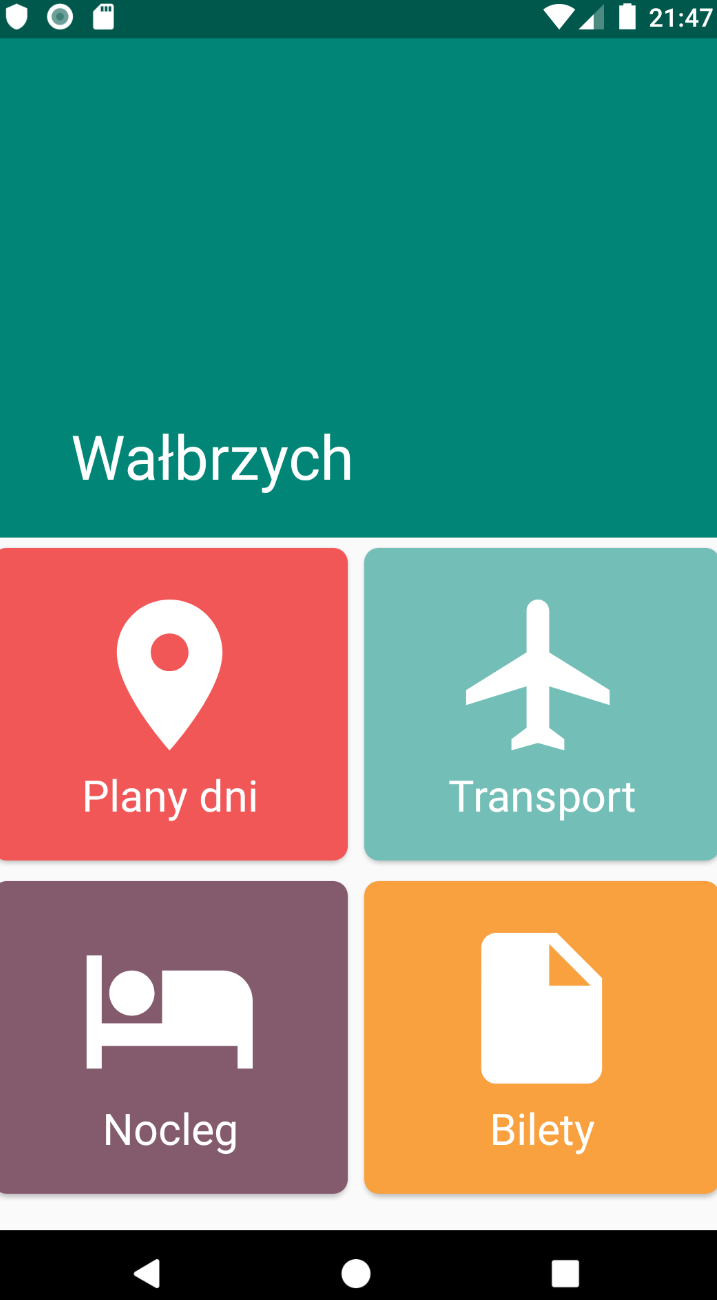
\includegraphics[width=0.8\linewidth, width=5cm]{firstDesign2}
\caption{Widok podróży}
\label{fig:firstDesign2}
\end{subfigure}
\begin{subfigure}{0.3\textwidth}
\centering
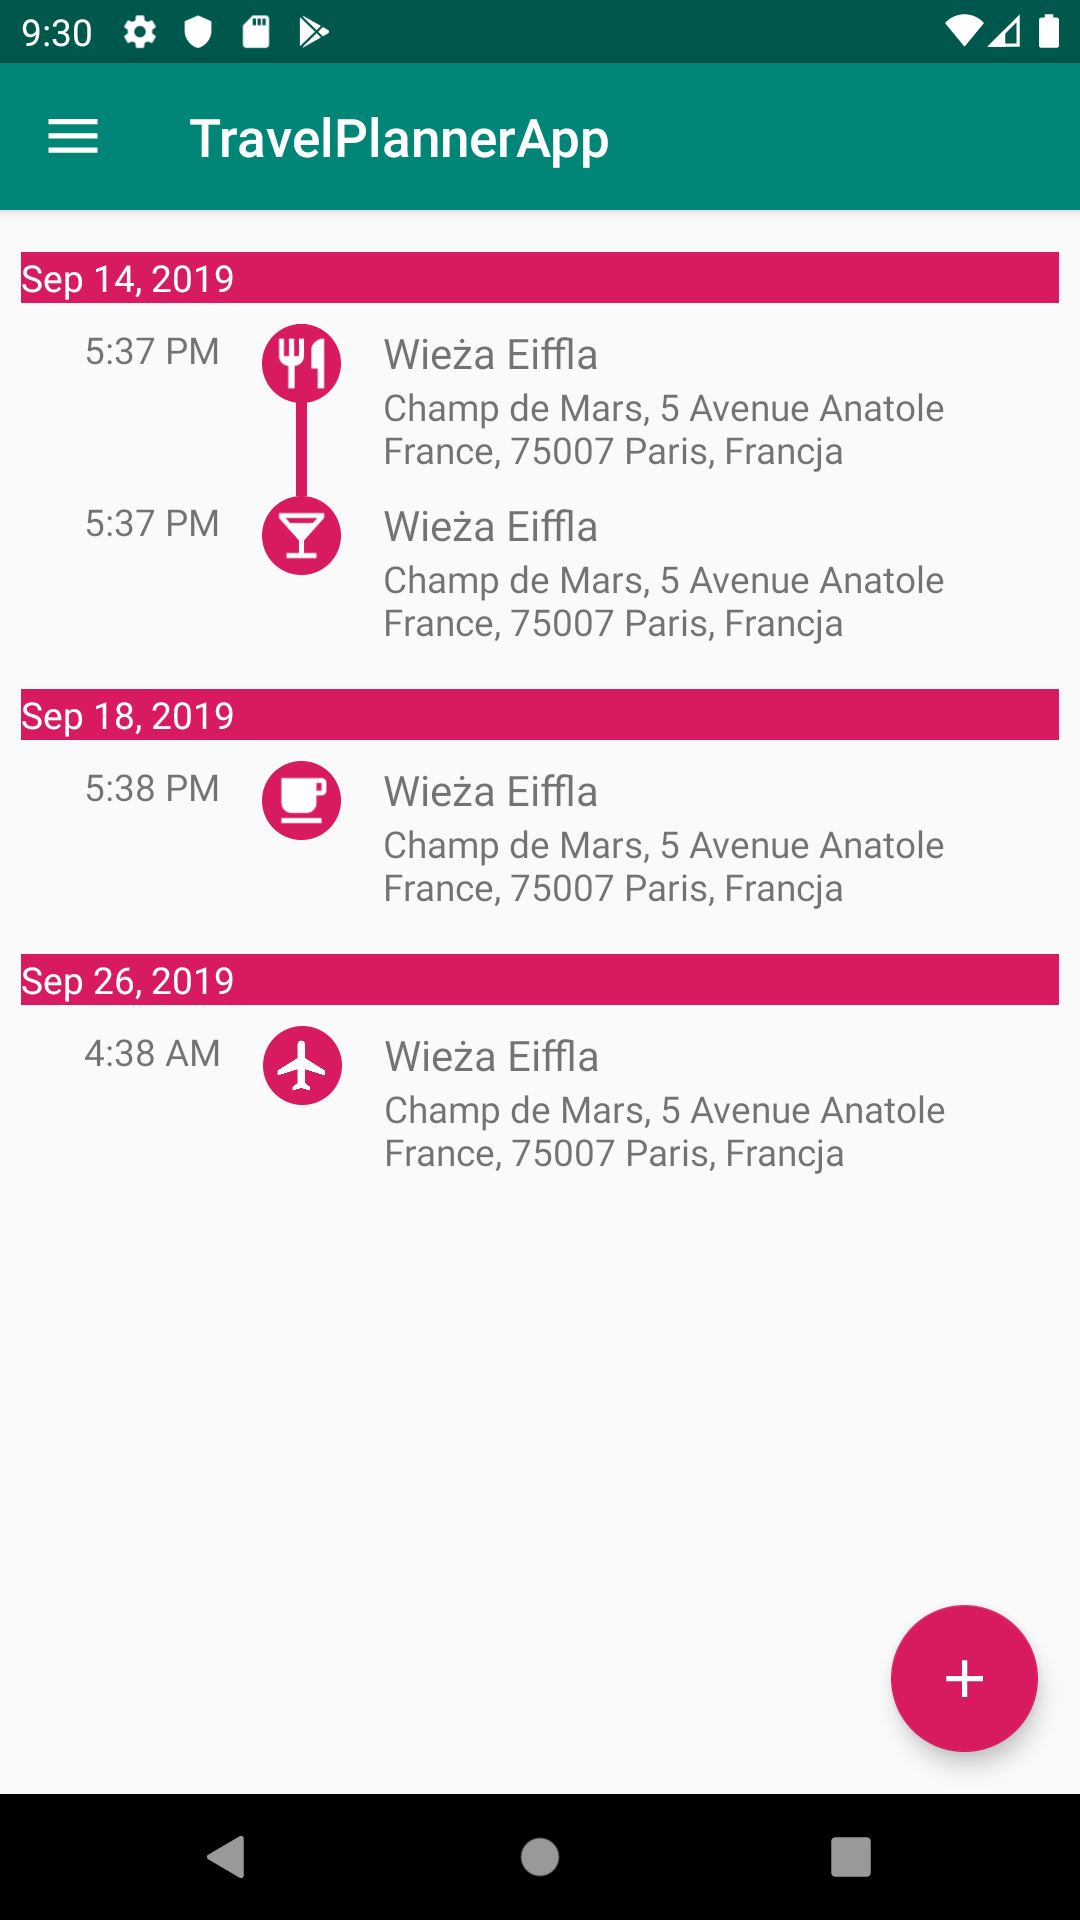
\includegraphics[width=0.8\linewidth, width=5cm]{firstDesign3}
\caption{Plan podróży}
\label{fig:firstDesign3}
\end{subfigure}
\caption{Pierwszy design}
\label{fig:podrecznik10}
\end{figure}
\FloatBarrier

\section{Rejestracja oraz logowanie użytkownika}
Użytkownik pierwszy raz uruchamiający aplikację i chcący z niej korzystać powinien stworzyć własne konto. W tym celu należy:

\begin{enumerate}

\item Kliknąć przycisk "Zarejestruj się"
\item W widoku rejestracji podać swój adres mailowy oraz hasło
\item Kliknąć "Zarejestruj się"
\item Po pojawieniu się powiadomienia "Twoje konto zostało utworzone" następuje automatyczne przekierowanie do widoku logowania
\item Uzupełnić pola widoku logowania tymi samymi danymi
\item Logowanie następuje w momencie uzupełnienia danych oraz kliknięcia „Zaloguj się”

\end{enumerate}

\begin{figure}[h]
\begin{subfigure}{0.5\textwidth}
\centering
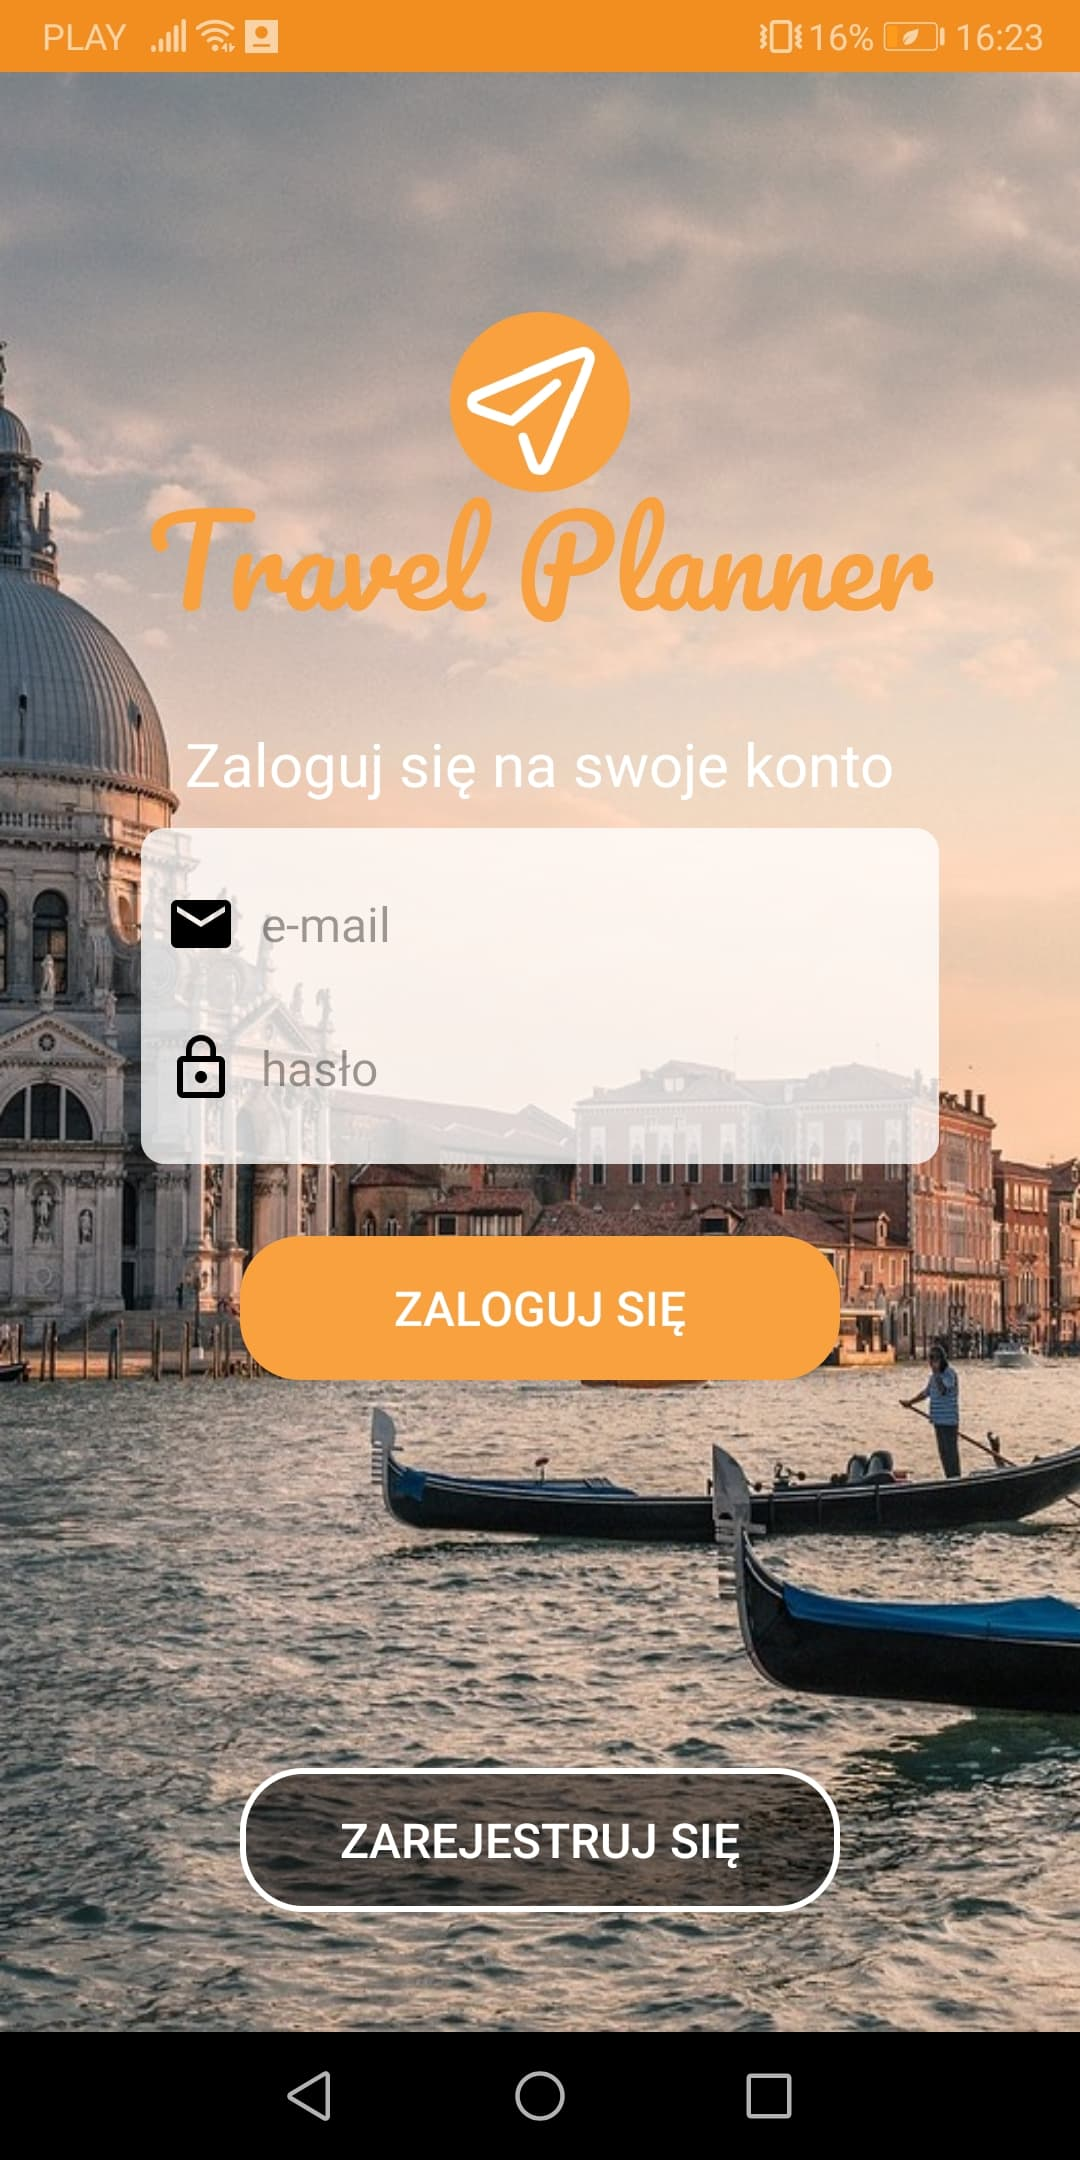
\includegraphics[width=0.9\linewidth, width=5cm]{loginView}
\caption{Widok logowania}
\label{fig:loginView}
\end{subfigure}
\begin{subfigure}{0.5\textwidth}
\centering
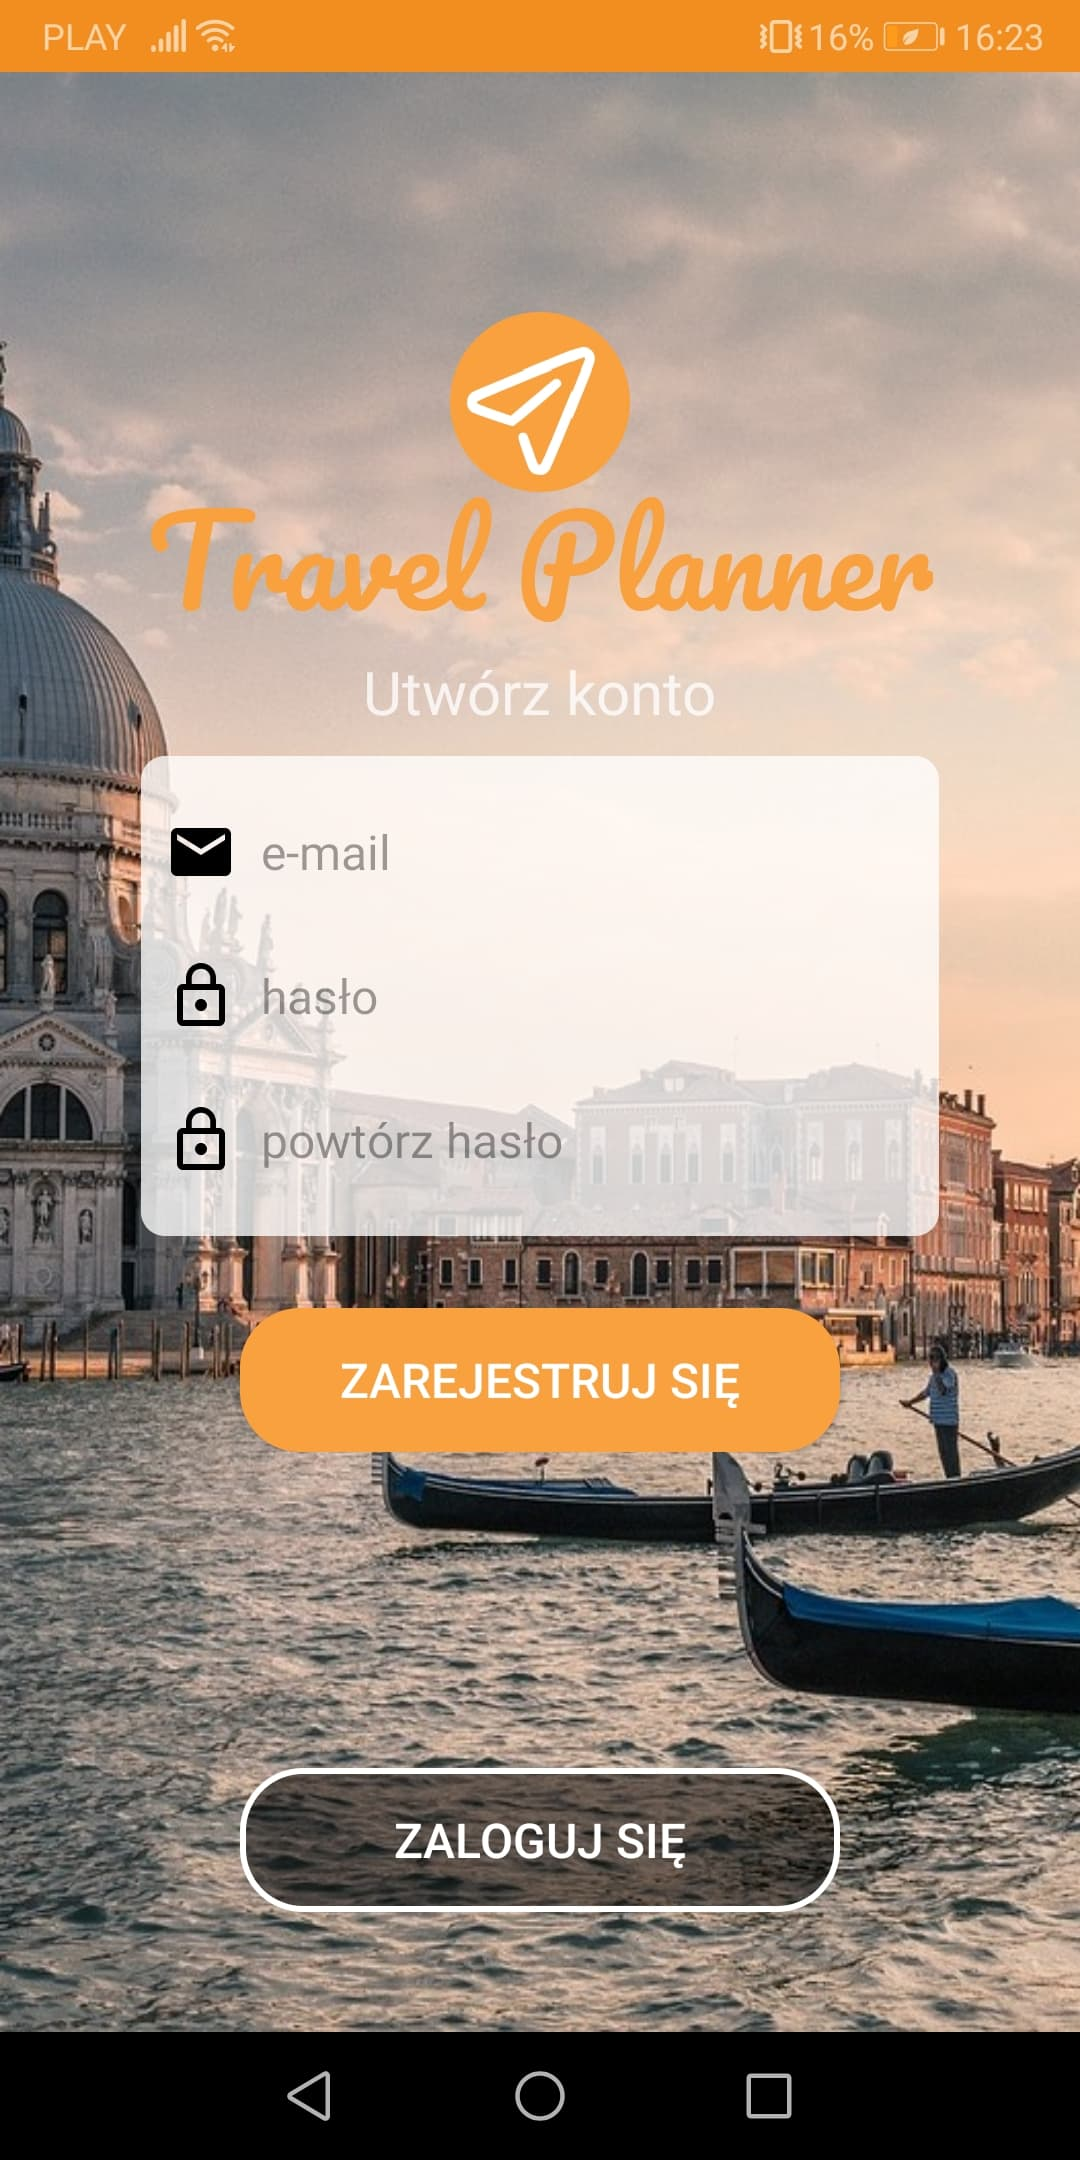
\includegraphics[width=0.9\linewidth, width=5cm]{registrationPage}
\caption{Widok rejestracji}
\label{fig:registrationPage}
\end{subfigure}
\caption{Logowanie i rejestracja użytkownika}
\label{fig:podrecznik1}
\end{figure}
\FloatBarrier

\section{Podróże}
Pierwszy widok pojawiający się tuż po zalogowaniu zawiera listę dostępnych podróży.

\begin{figure}[h]
\centering
\begin{subfigure}{0.3\textwidth}
\centering
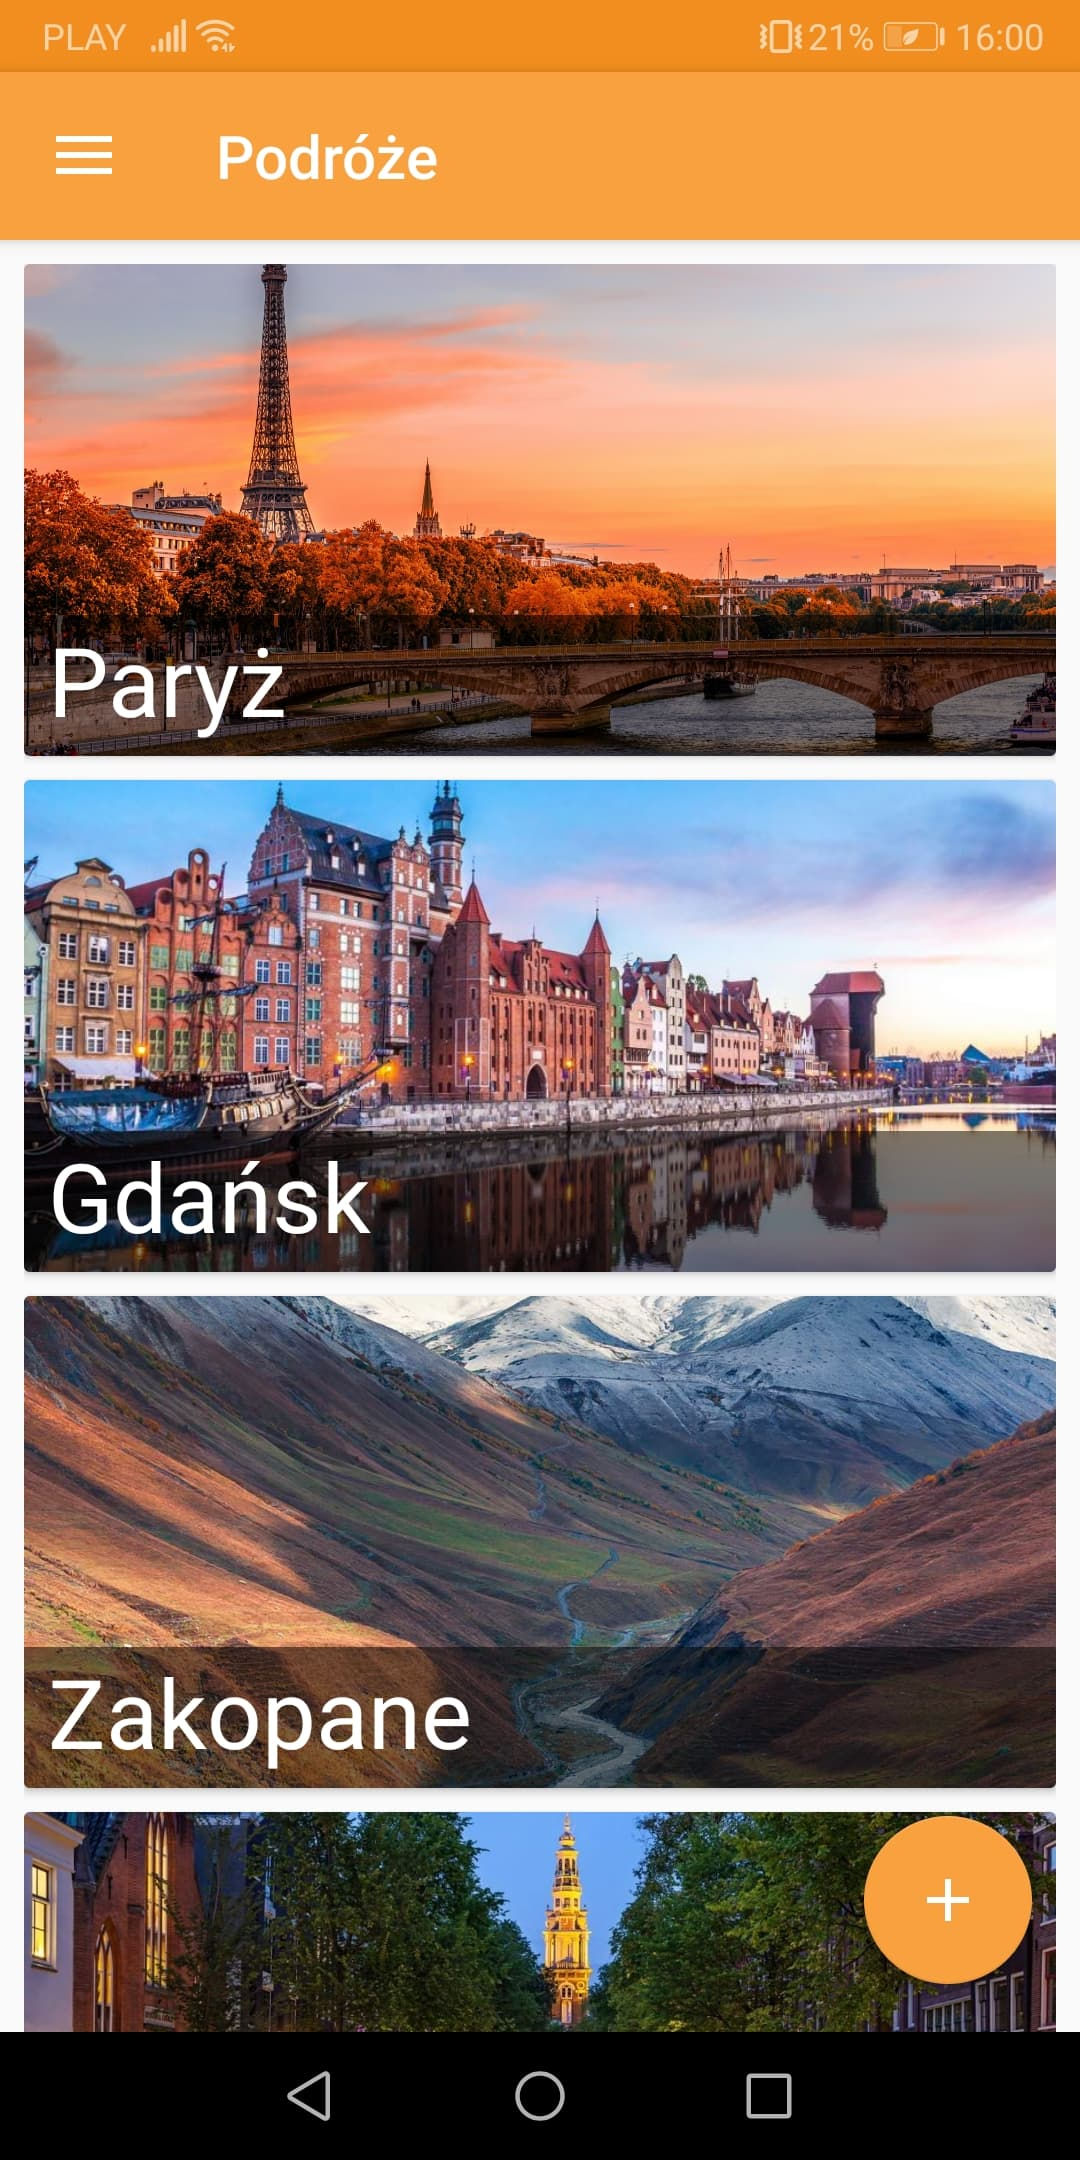
\includegraphics[width=0.8\linewidth, width=5cm]{travelsView}
\caption{Widok podróży użytkownika}
\label{fig:travelsView}
\end{subfigure}
\begin{subfigure}{0.3\textwidth}
\centering
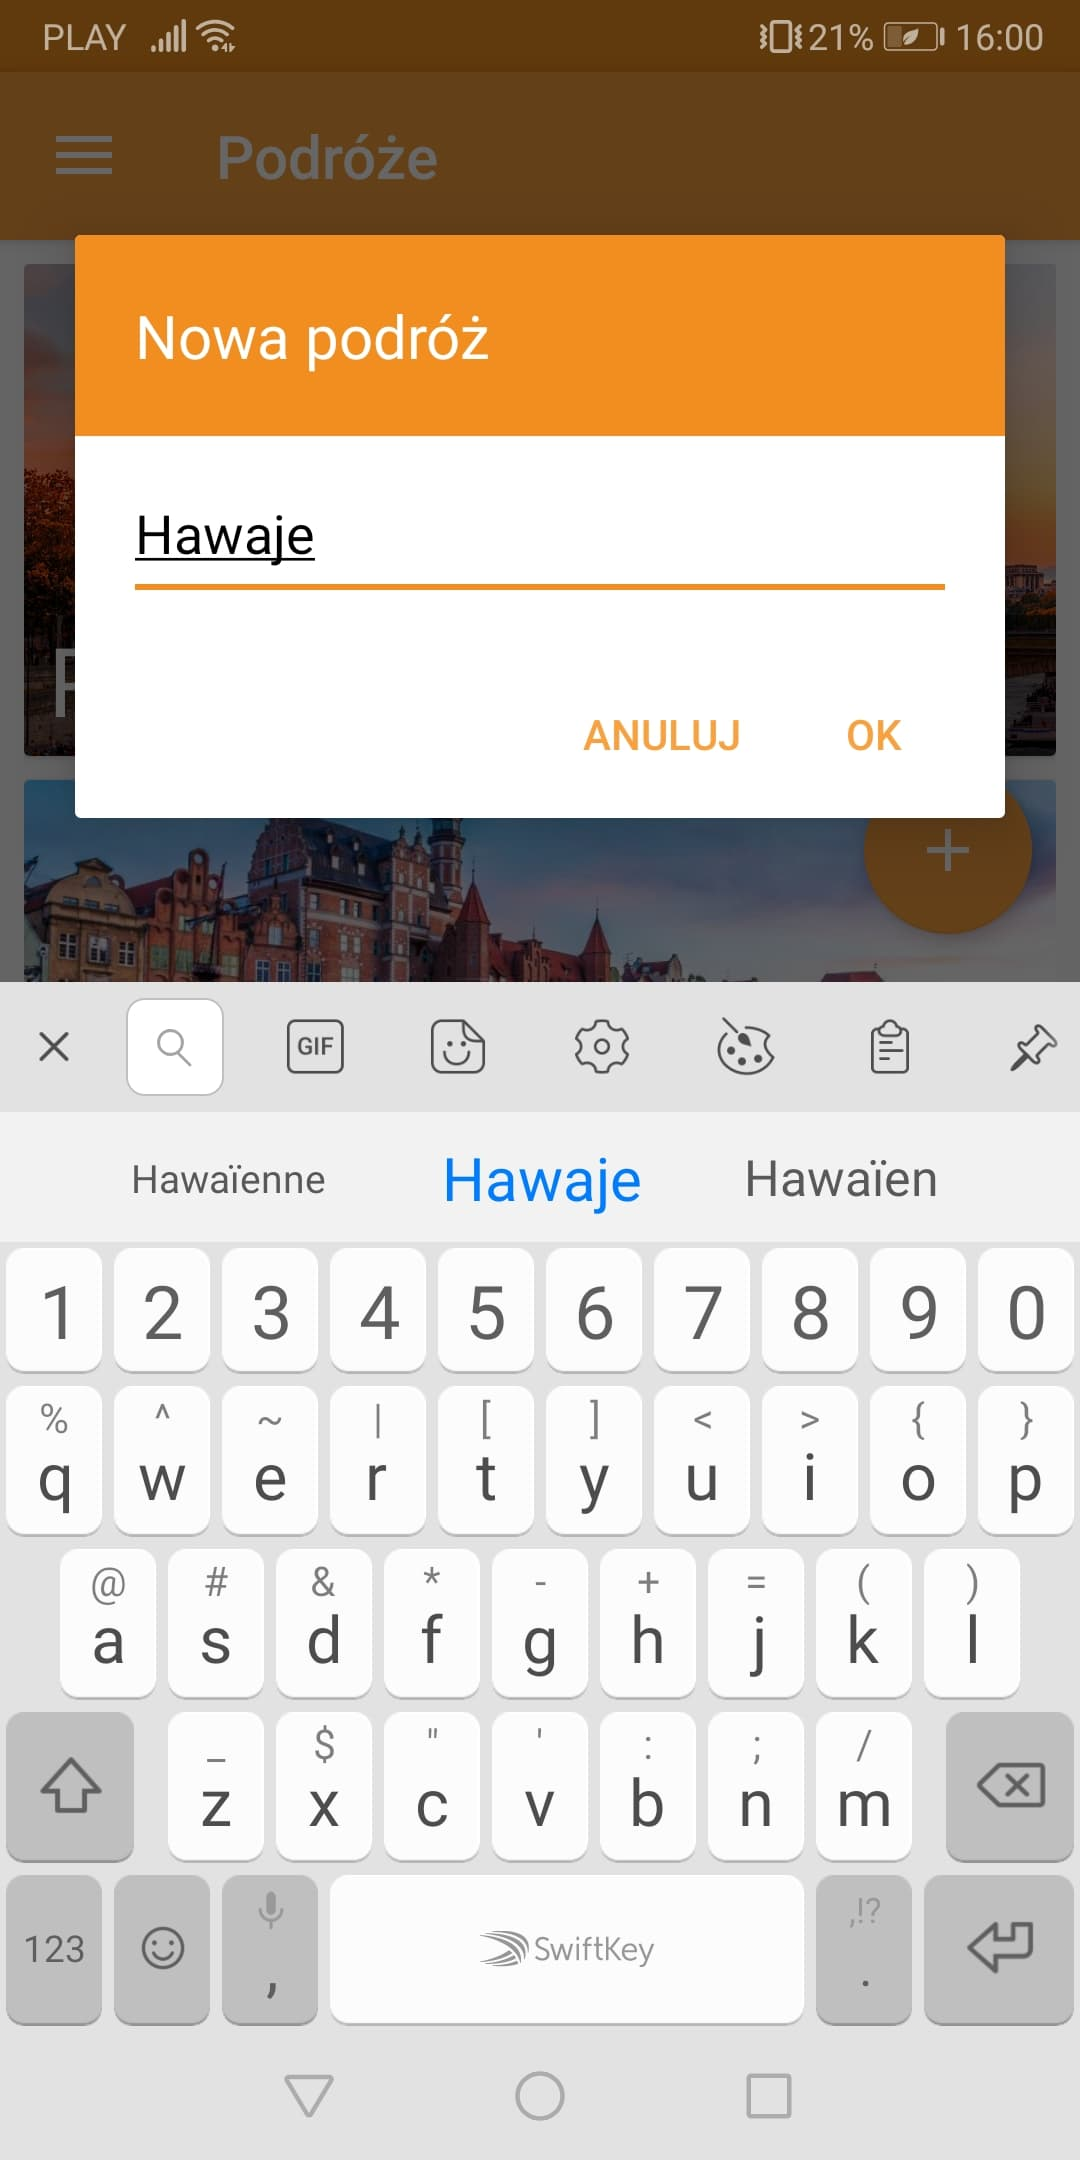
\includegraphics[width=0.8\linewidth, width=5cm]{createNewTravel}
\caption{Okno dialogowe}
\label{fig:createNewTravel}
\end{subfigure}
\begin{subfigure}{0.3\textwidth}
\centering
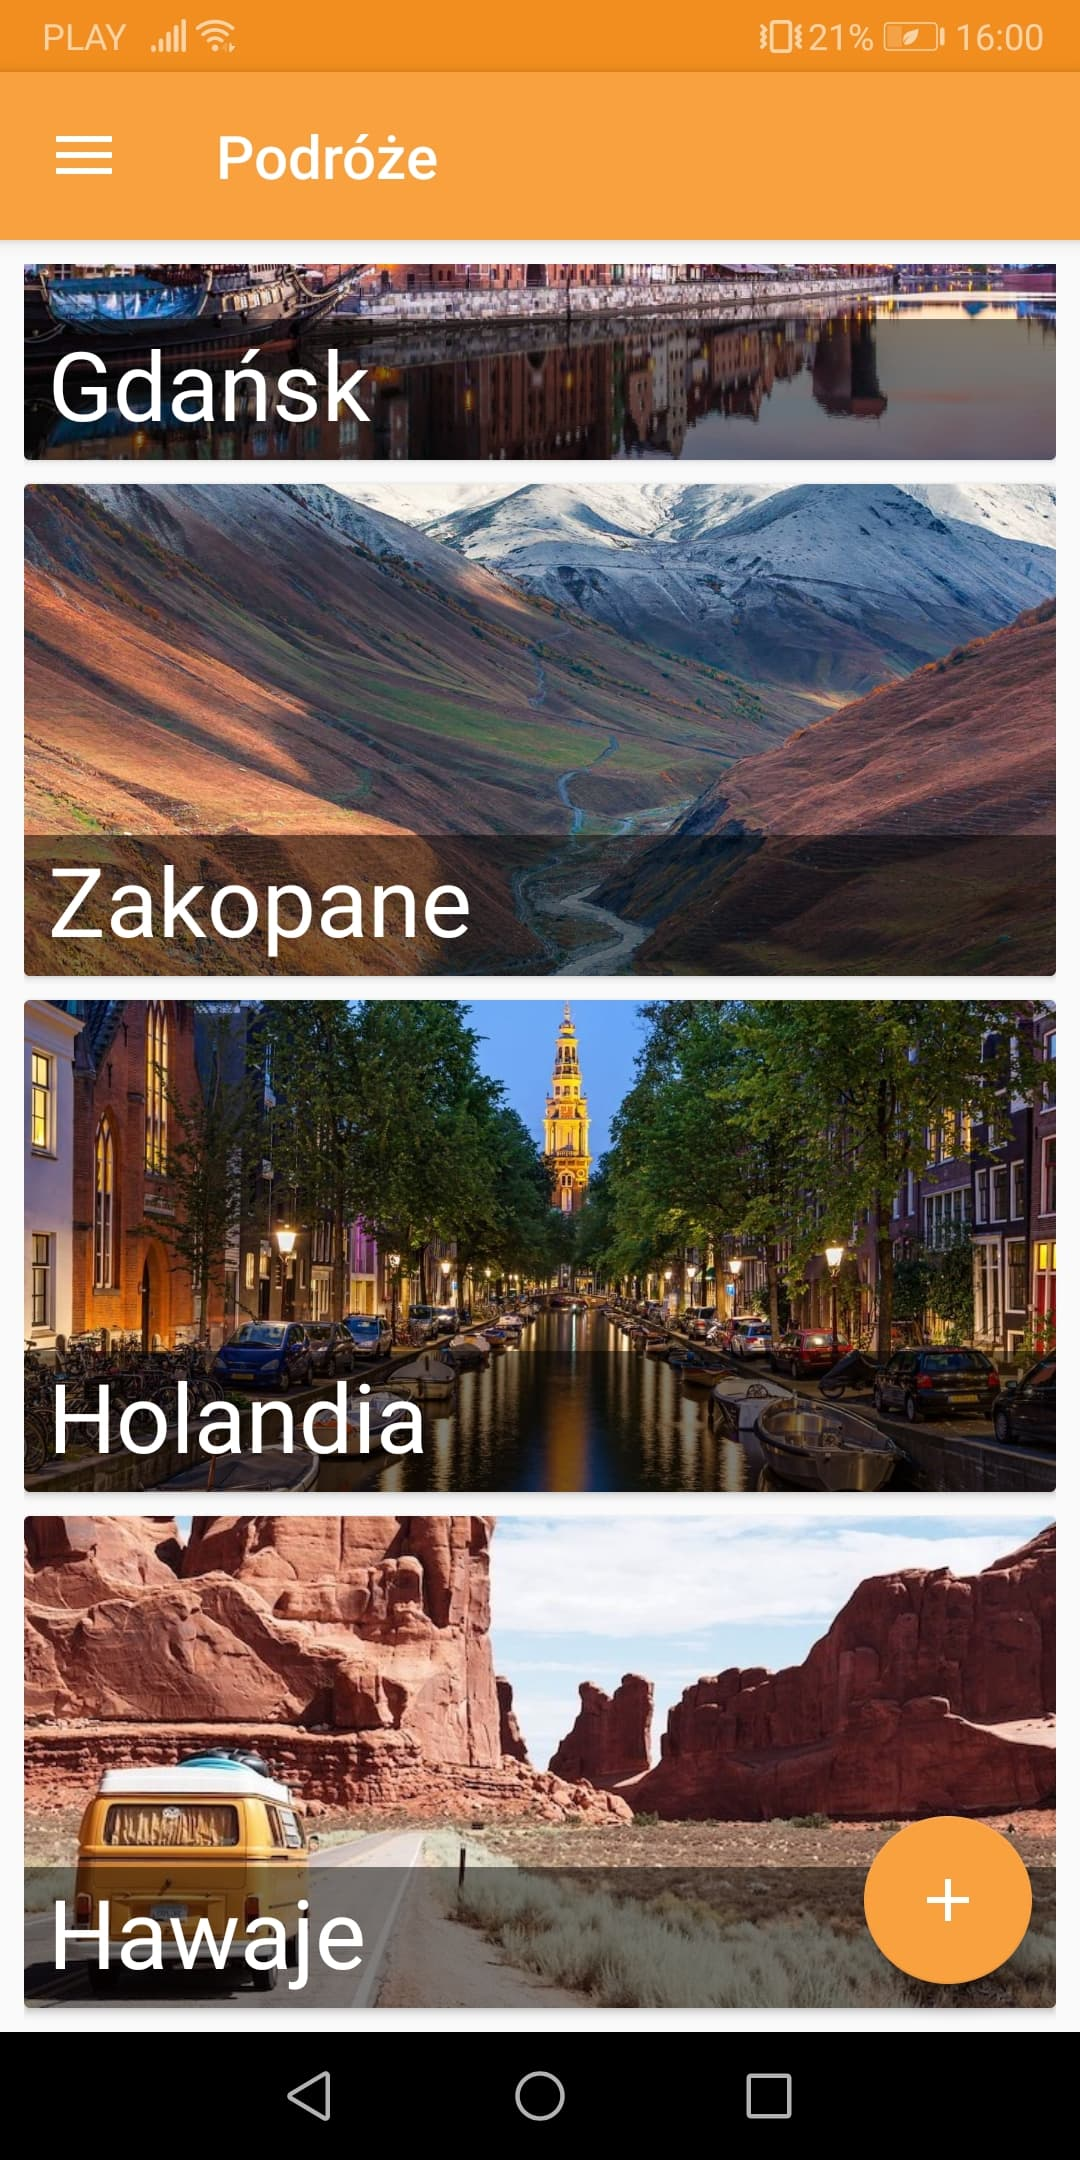
\includegraphics[width=0.8\linewidth, width=5cm]{defaultImage}
\caption{Domyślny obraz podróży}
\label{fig:defaultImage}
\end{subfigure}
\caption{Tworzenie nowej podróży}
\label{fig:podrecznik3}
\end{figure}
\FloatBarrier

\subsection{Tworzenie podróży}
W celu utworzenia podróży należy:
\begin{enumerate}
\item Nacisnąć przycisk oznaczony symbolem „+”
\item Uzupełnić okno dialogowe nazwą podróży i kliknąć "OK"
\item Utworzona podróż pojawi się na liście wraz z domyślnym zdjęciem
\end{enumerate}


\section{Widok podróży}
Po wybraniu danej podróży zostaje wyświetlony widok zawierający informacje na jej temat.

\begin{figure}[h]
\centering
\begin{subfigure}{0.4\textwidth}
\centering
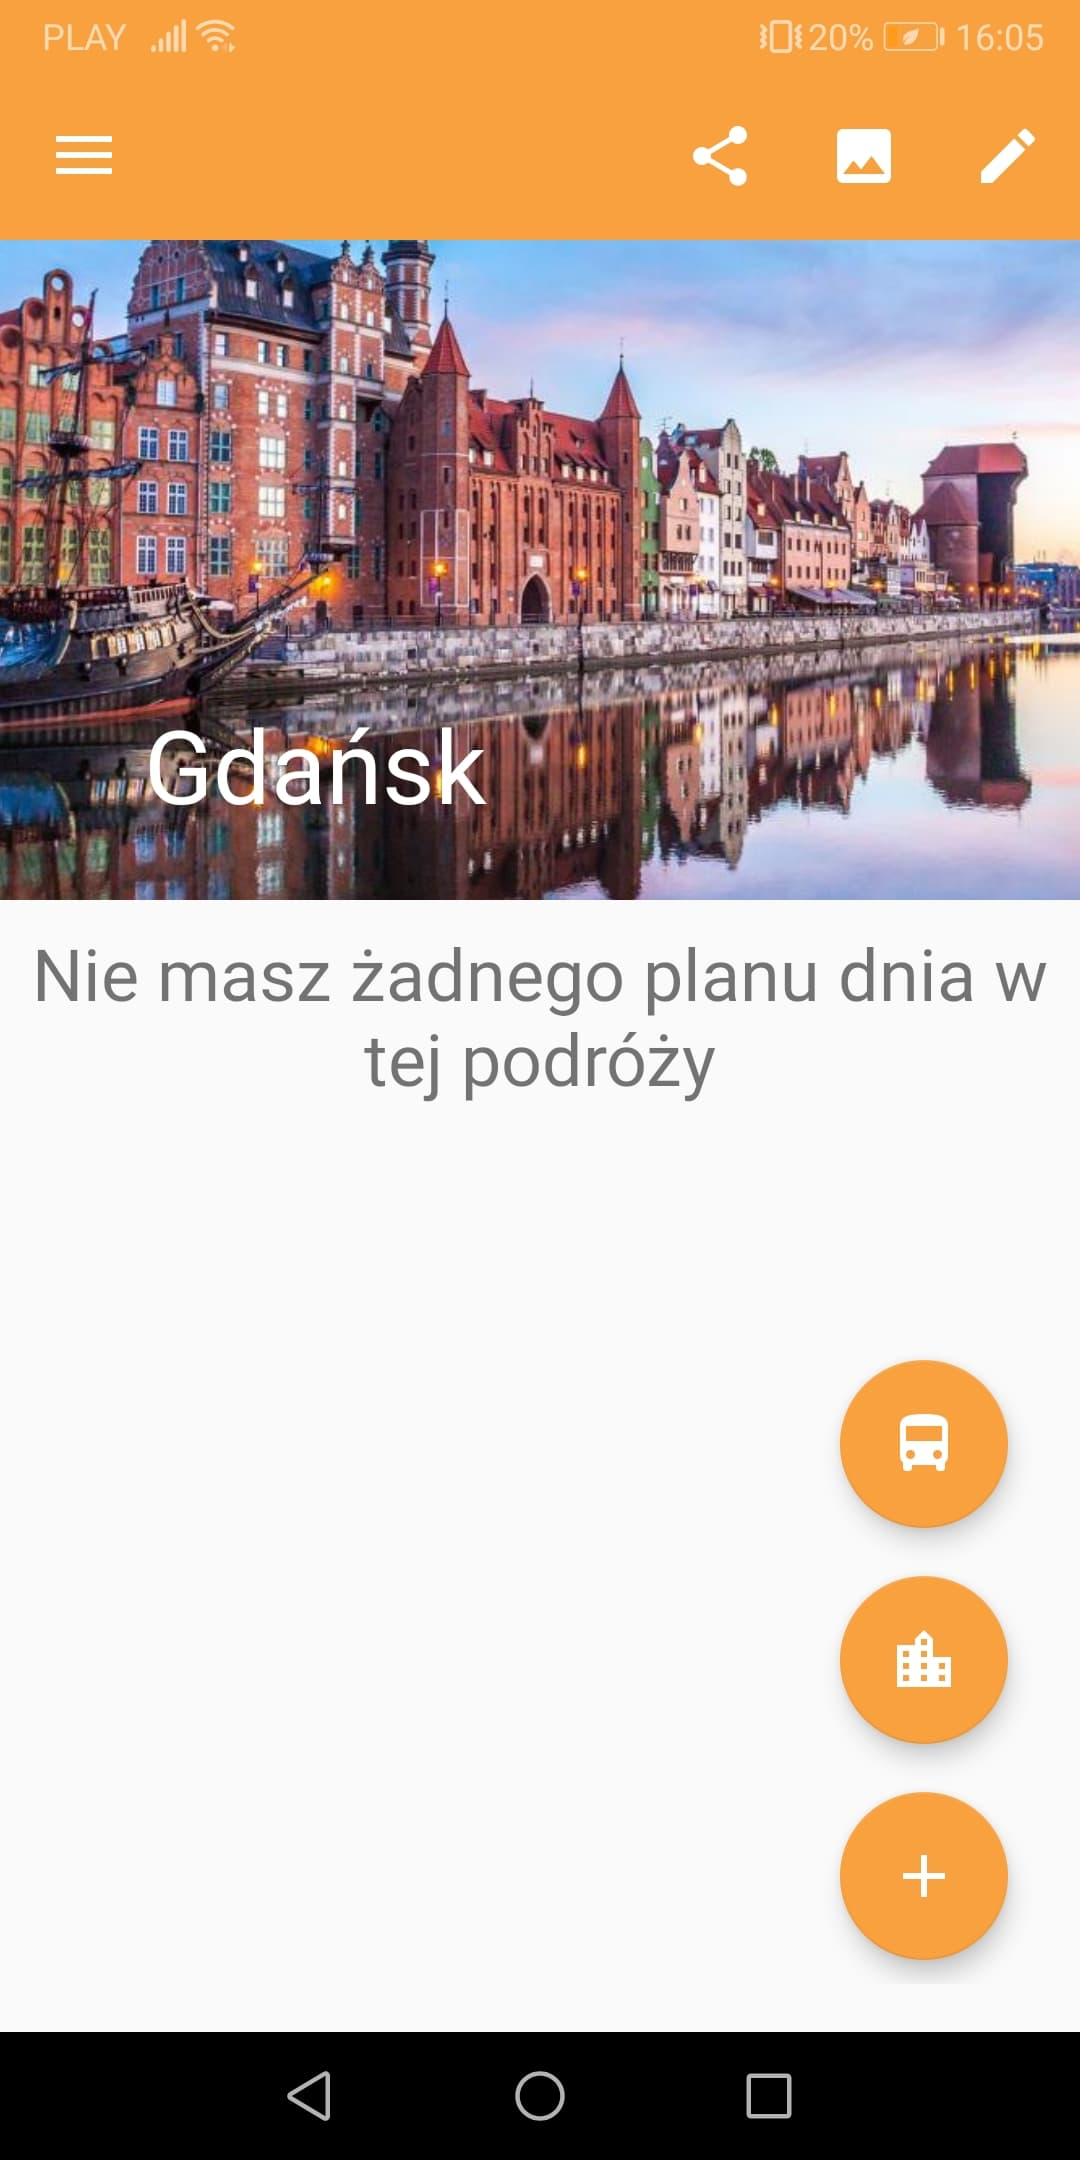
\includegraphics[width=0.9\linewidth, width=5cm]{newTravel}
\caption{Widok danej podróży}
\label{fig:newTravel}
\end{subfigure}
\begin{subfigure}{0.4\textwidth}
\centering
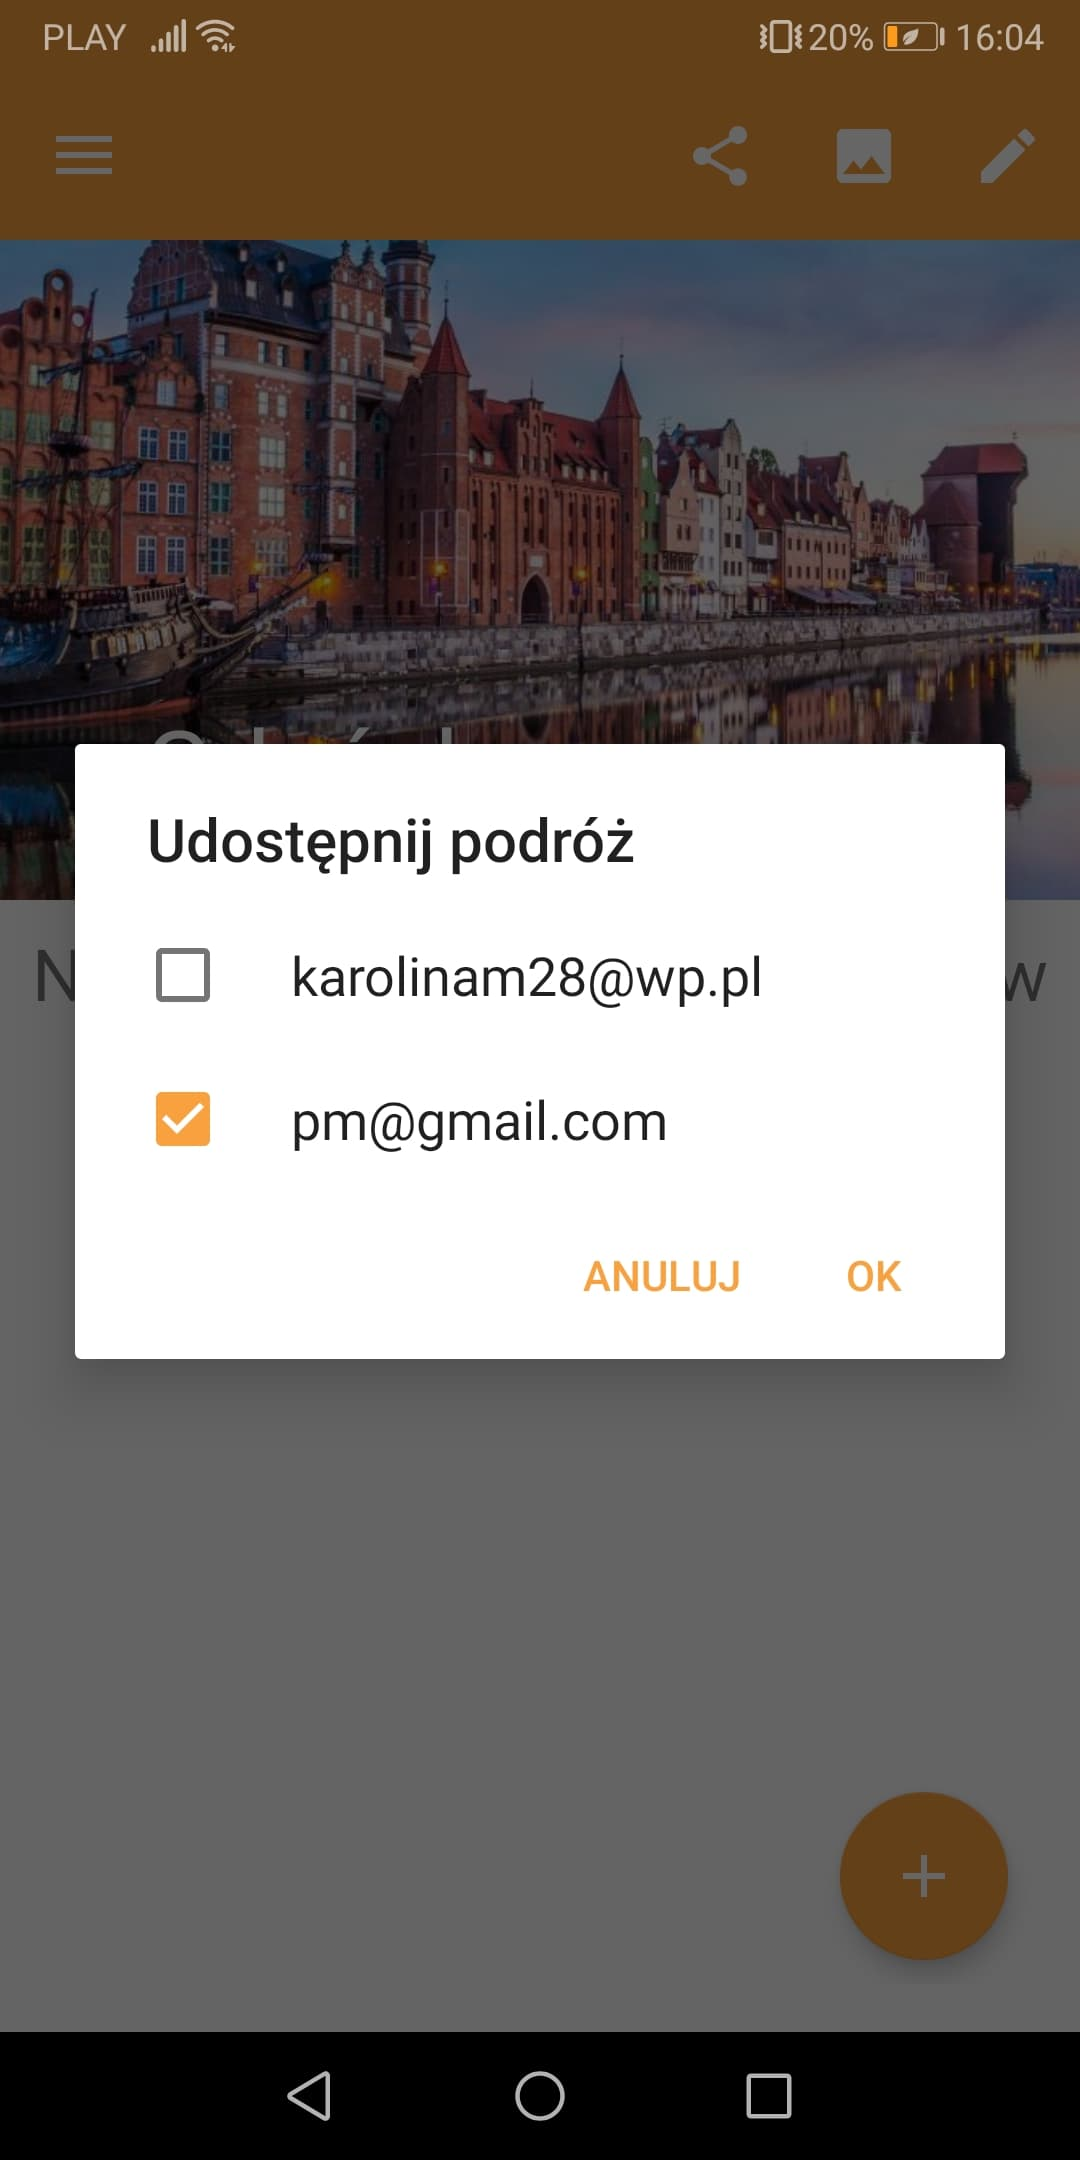
\includegraphics[width=0.9\linewidth, width=5cm]{shareTravelDialog}
\caption{Udostępnianie podróży znajomym}
\label{fig:shareTravelDialog}
\end{subfigure}
\caption{Pojedyńcza podróż}
\label{fig:podrecznik4}
\end{figure}
\FloatBarrier
\subsection{Zmiana nazwy podróży}

W celu zmiany nazwy podróży należy:
\begin{enumerate}
\item Nacisnąć przycisk oznaczony symbolem ołówka
\item Uzupełnić okno dialogowe nową nazwą podróży i kliknąć "OK"
\item Nazwa podróży zostanie zaktualizowana
\end{enumerate}

\subsection{Zmiana tła podróży}

W celu zmiany tła podróży należy:
\begin{enumerate}
\item Nacisnąć przycisk oznaczony symbolem zdjęcia
\item Wybrać odpowiednie zdjęcie z galerii urządzenia
\item Zdjęcie zostanie zaktualizowane
\end{enumerate}

\subsection{Udostępnianie podróży znajomym}

W celu udostępnienia podróży znajomym należy:
\begin{enumerate}
\item Nacisnąć przycisk oznaczony symbolem udostępniania
\item Wybrać wszystkich znajomych, którym ma zostać udostępniona podróż
\item Potwierdzić swój wybór poprzez naciśnięcie przycisku "OK"
\item W przypadku potwierdzenia wykonania czynności pojawi się powiadomienie z odpowiednim komunikatem
\end{enumerate}

\subsection{Dodanie elementu planu dnia}
W celu dodania elementu planu dnia należy:
\begin{enumerate}
\item Nacisnąć przycisk oznaczony symbolem "+"
\item Wybrać jedną z dwóch dostępnych opcji
\end{enumerate}
\paragraph{Dodanie miejsca}
Pierwsza z opcji jest oznaczona poprzez symbol budynku.
Umożliwia on dodanie miejsca do planu dnia.

\begin{enumerate}
\item Należy wybrać kategorię spośród:
\begin{itemize}
\item Jedzenie i picie
\item Restauracja
\item Fast food
\item Kawiarnia
\item Rozrywka
\item Zabytki i muzea
\item Lotnisko
\item Nocleg
\item Zakupy
\item Aktywny wypoczynek
\item Natura
\item Stacja paliw
\item Bankomat
\item Toaleta
\item Opieka zdrowotna
\end{itemize}
\item Po naciśnięciu wyszukiwania miejsca po nazwie pojawia się widok mapy umożliwiającej wybranie konkretnego miejsca
\item Po wybraniu pinezki pojawiają się dokładne informacje na temat miejsca
\item Naciśnięcie przycisku zawierającego symbol „tick” przekierowuje użytkownika do pierwszego ekranu wyszukiwania
\item Następnie należy wybrać datę oraz godzinę realizacji planu
\item Opcjonalne jest dodanie własnych notatek
\item Dodanie miejsca następuje po naciśnięciu przycisku oznaczonym symbolem "tick"
\end{enumerate}

\begin{figure}[h]
\begin{subfigure}{0.3\textwidth}
\centering
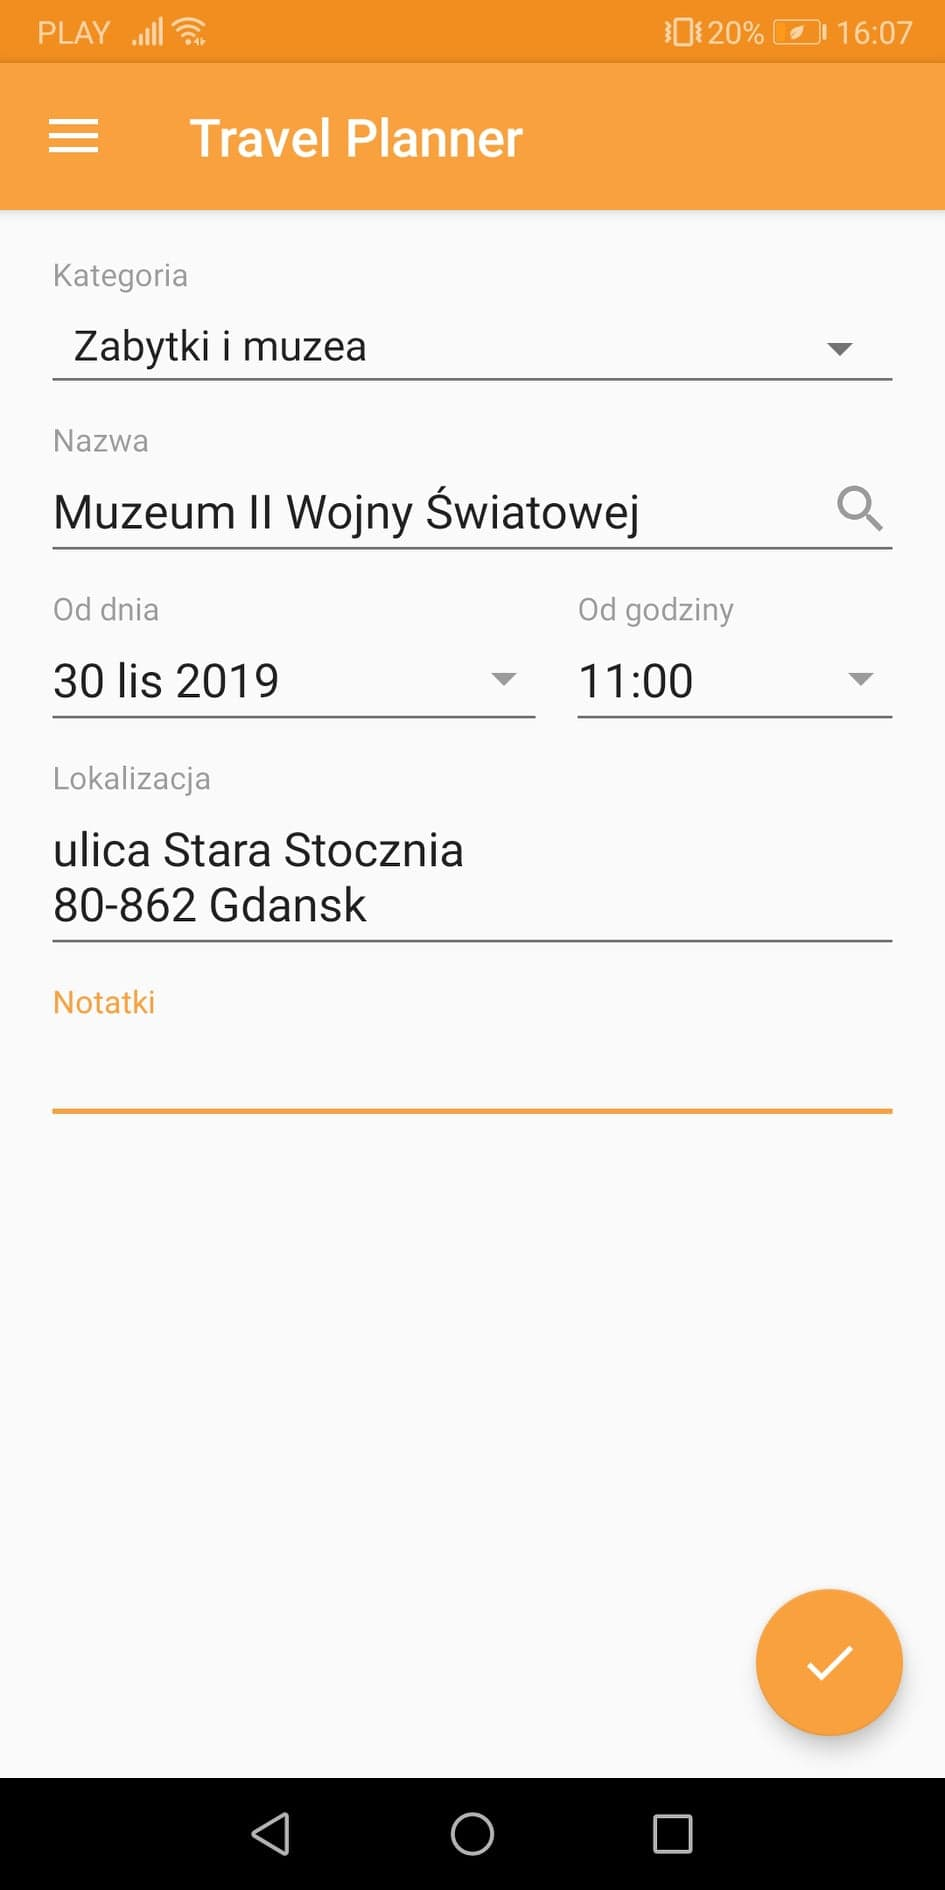
\includegraphics[width=0.9\linewidth, width=5cm]{searchPlace}
\caption{Uzupełnienie danych}
\label{fig:searchPlace}
\end{subfigure}
\begin{subfigure}{0.3\textwidth}
\centering
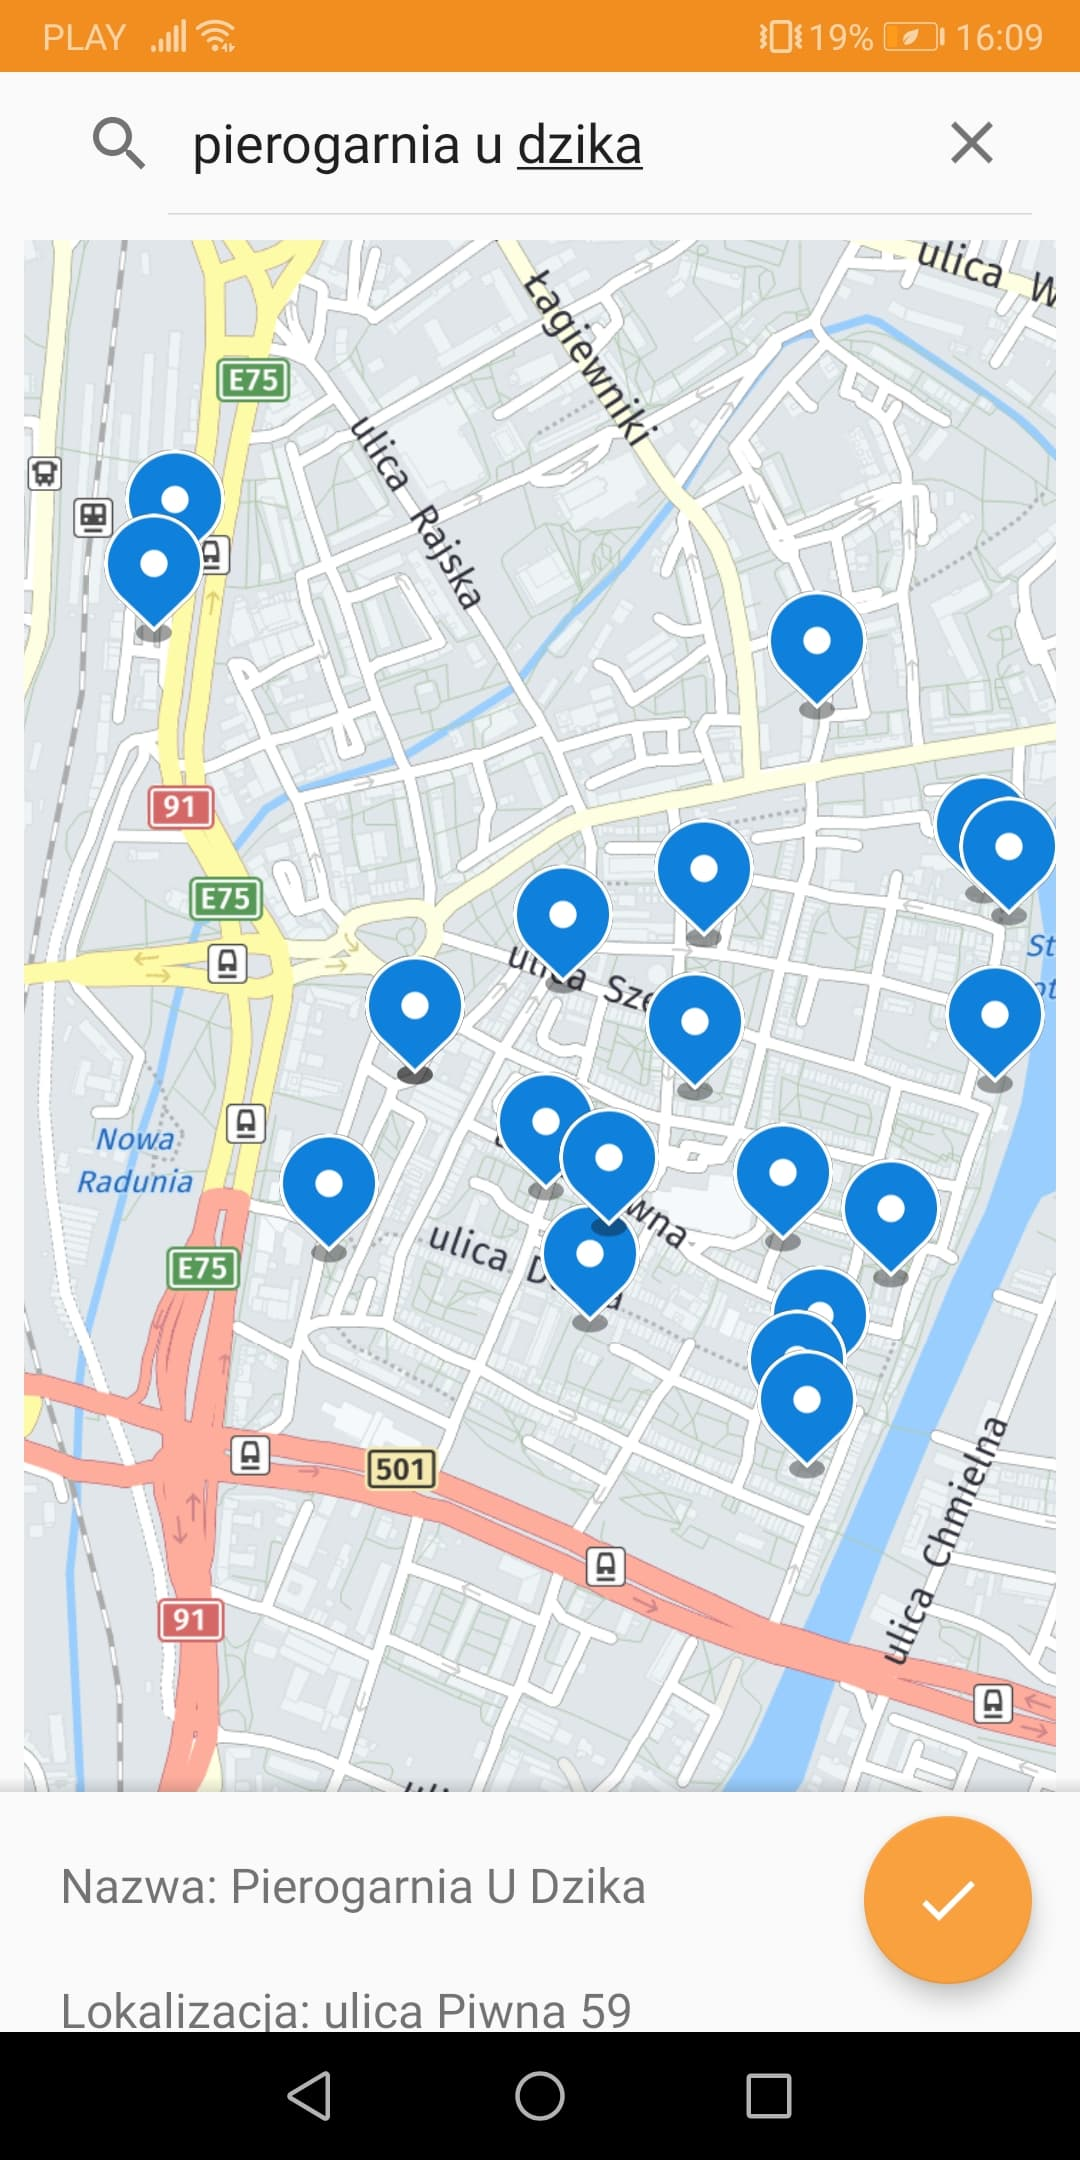
\includegraphics[width=0.9\linewidth, width=5cm]{searchingPlace}
\caption{Wyszukiwanie miejsca}
\label{fig:searchingPlace}
\end{subfigure}
\begin{subfigure}{0.3\textwidth}
\centering
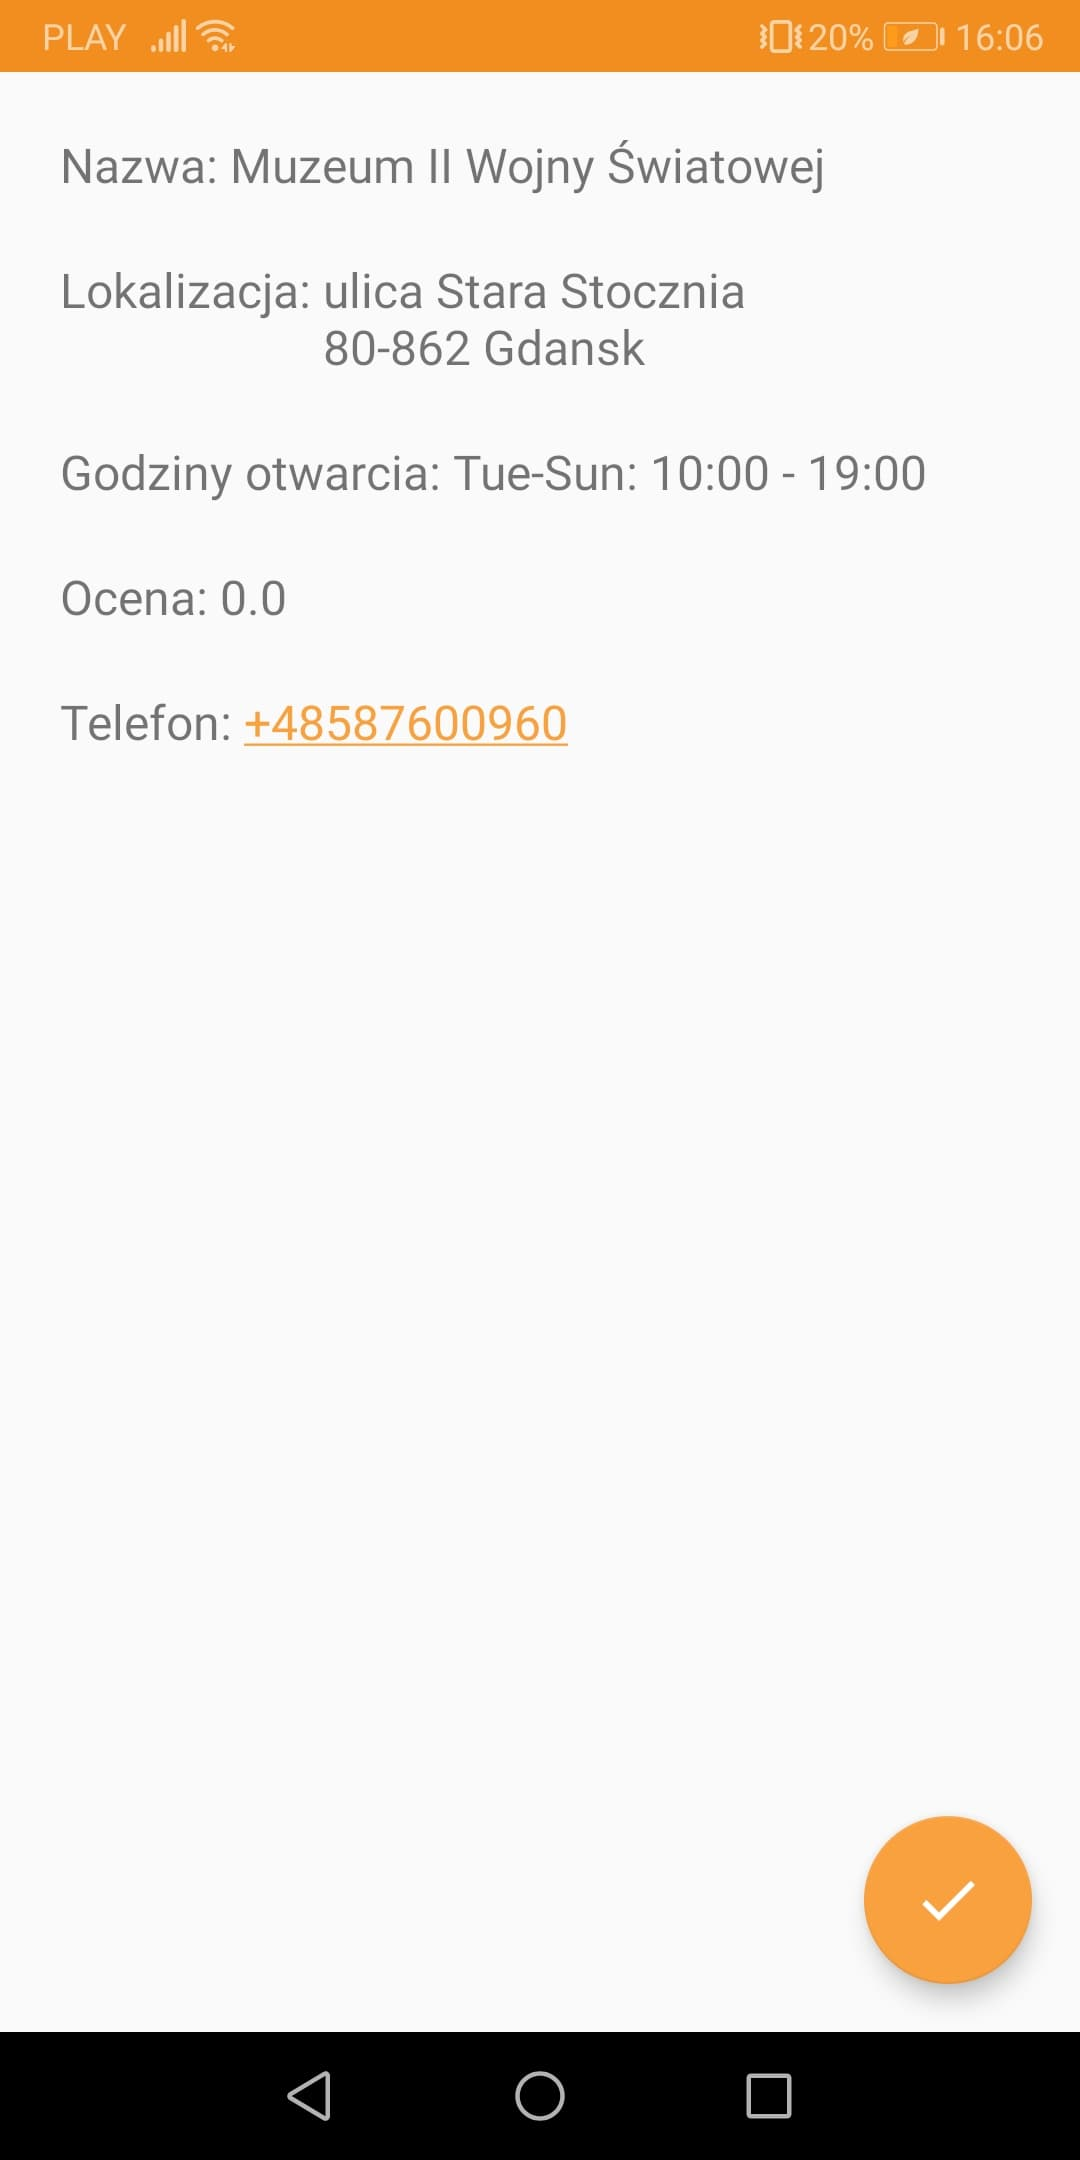
\includegraphics[width=0.9\linewidth, width=5cm]{placeDescription}
\caption{Szczegółowe informacje na temat miejsca}
\label{fig:placeDescription}
\end{subfigure}
\begin{subfigure}{0.5\textwidth}
\centering
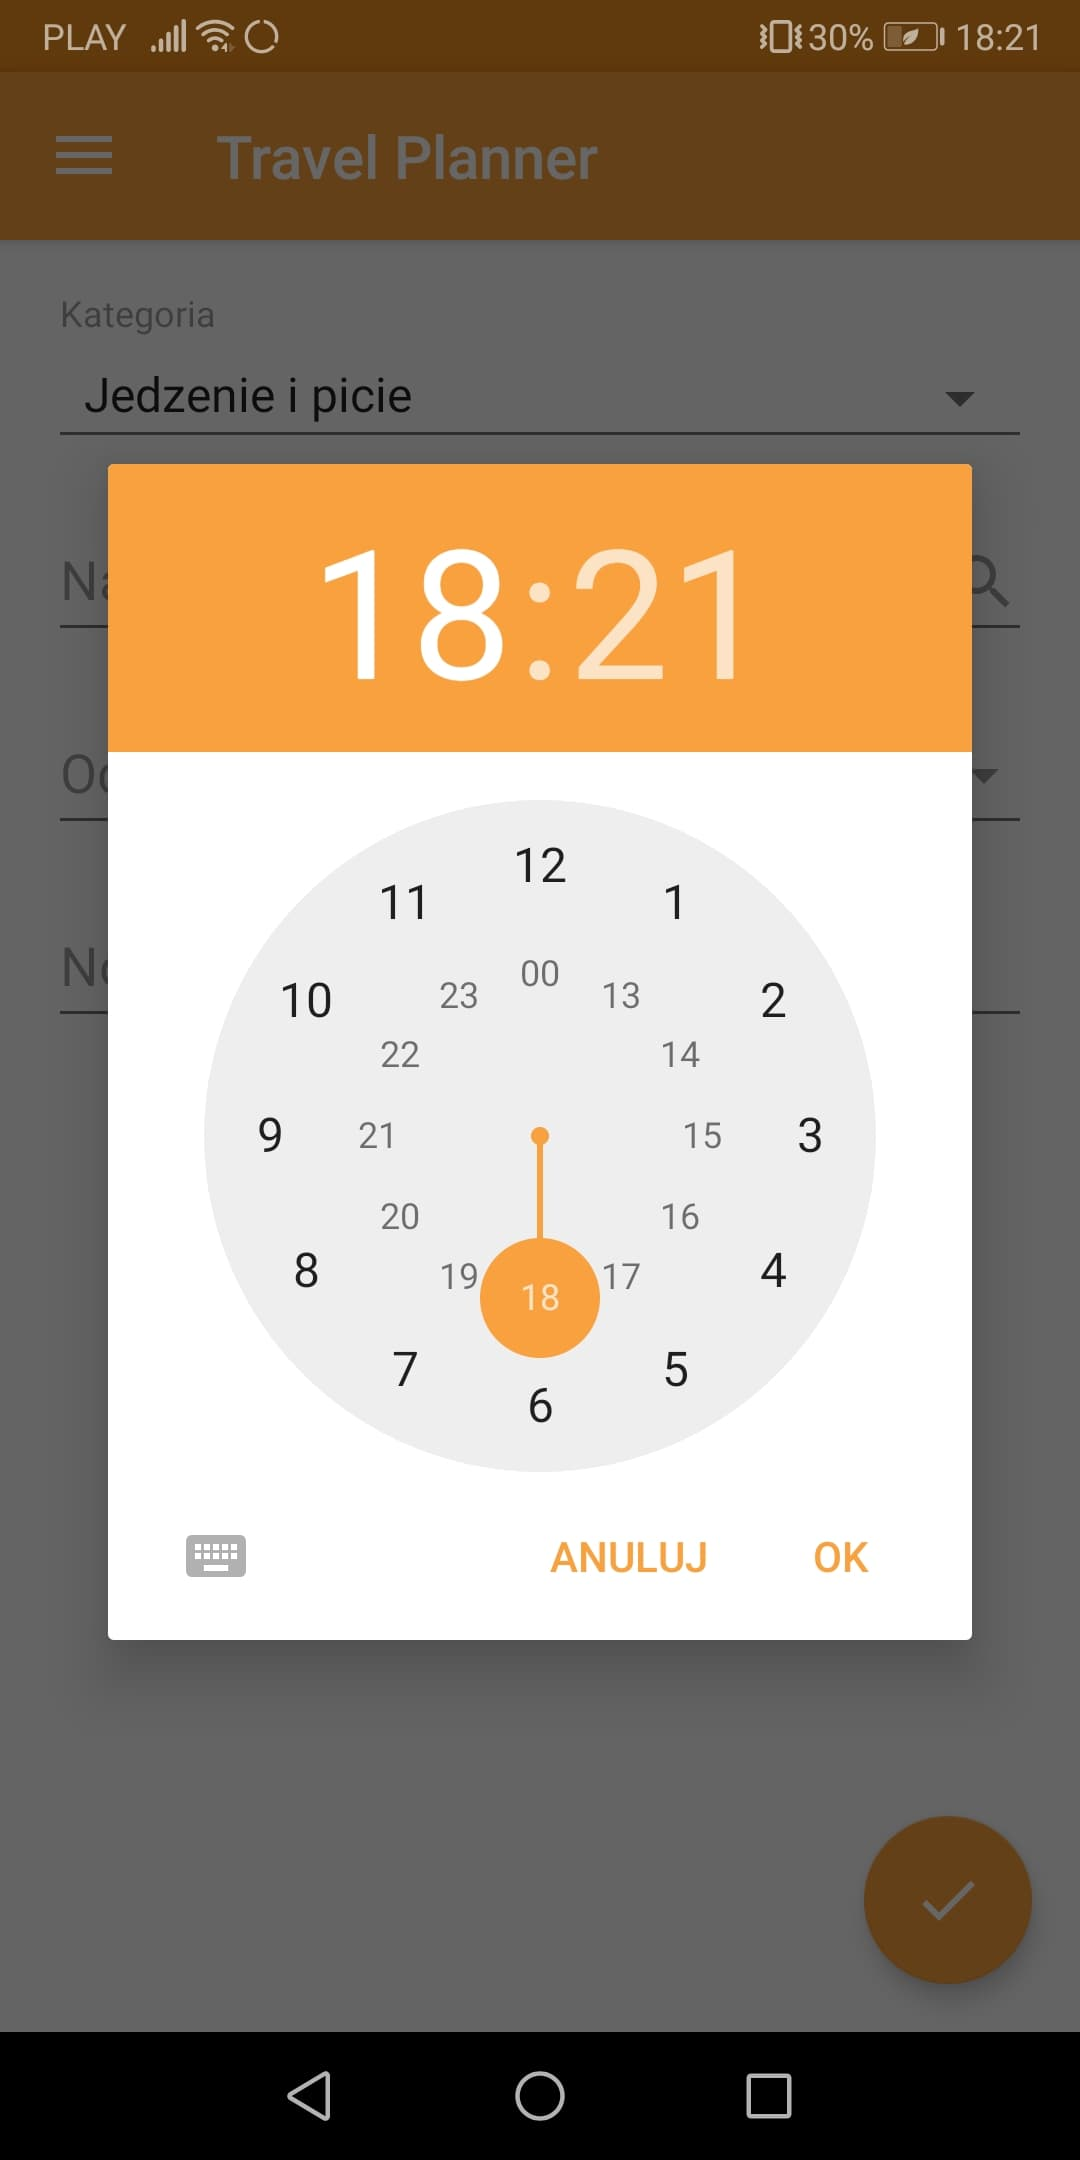
\includegraphics[width=0.9\linewidth, width=5cm]{clock}
\caption{Wybieranie godziny}
\label{fig:clock}
\end{subfigure}
\begin{subfigure}{0.5\textwidth}
\centering
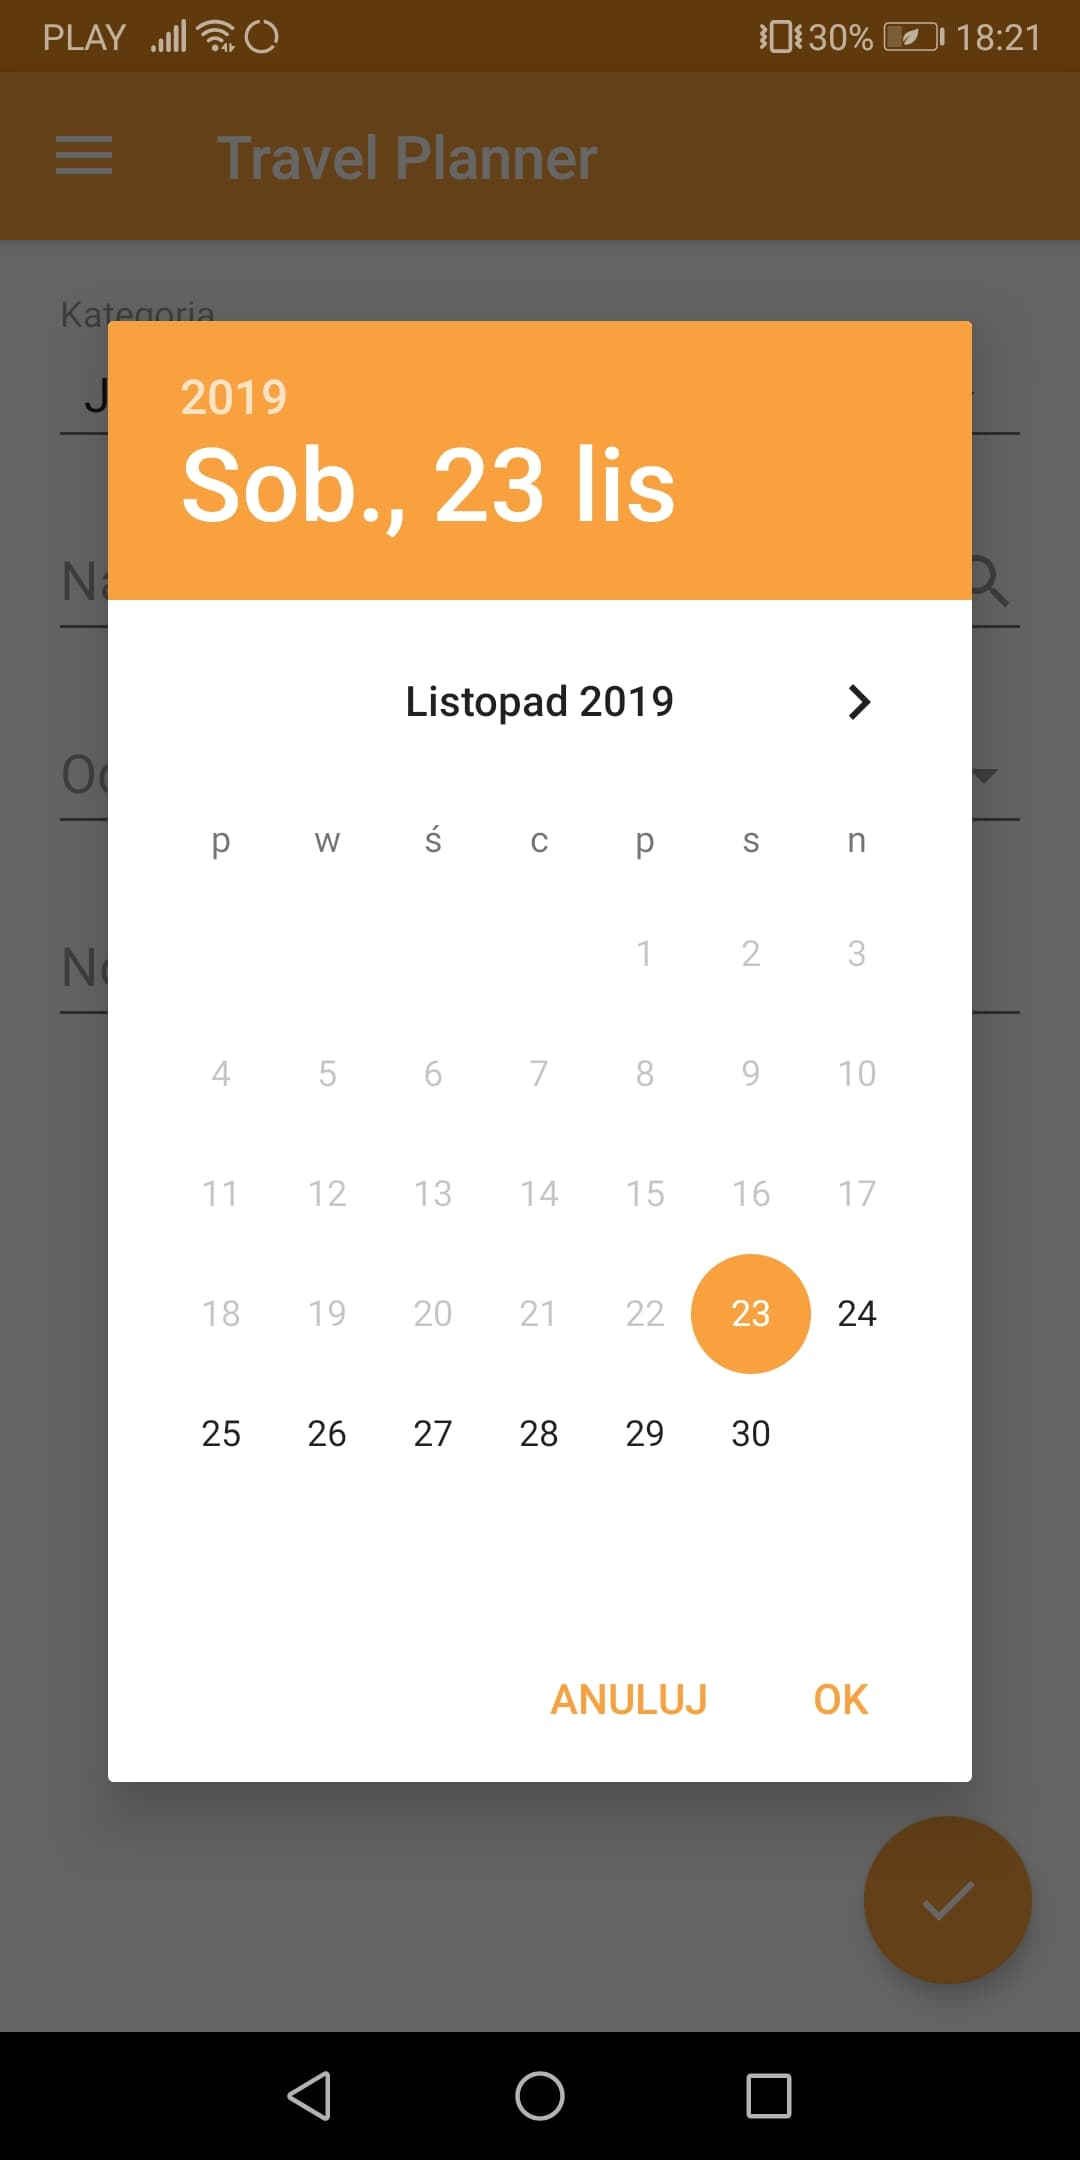
\includegraphics[width=0.9\linewidth, width=5cm]{calendar}
\caption{Wybieranie daty}
\label{fig:calendar}
\end{subfigure}
\caption{Tworzenie elementu planu dnia}
\label{fig:podrecznik7}
\end{figure}
\FloatBarrier
\paragraph{Dodanie transportu}
W przypadku wybrania przycisku z symbolem samochodu użytkownik ma możliwość dodania transportu jako element planu dnia.
\begin{enumerate}
\item Należy kliknąć na na pole miejsca początkowego
\item Następnie wybrać element planu dnia
\item Kliknąć na pole miejsca docelowego
\item Wybrać element planu dnia
\item Kliknąć na przycisk oznaczony symbolem strzałki w prawo
\item Wybrać rodzaj transportu
\item Kliknąć na przycisk oznaczony symbolem lupy
\end{enumerate}

\begin{figure}[h]
\centering
\begin{subfigure}{0.4\textwidth}
\centering
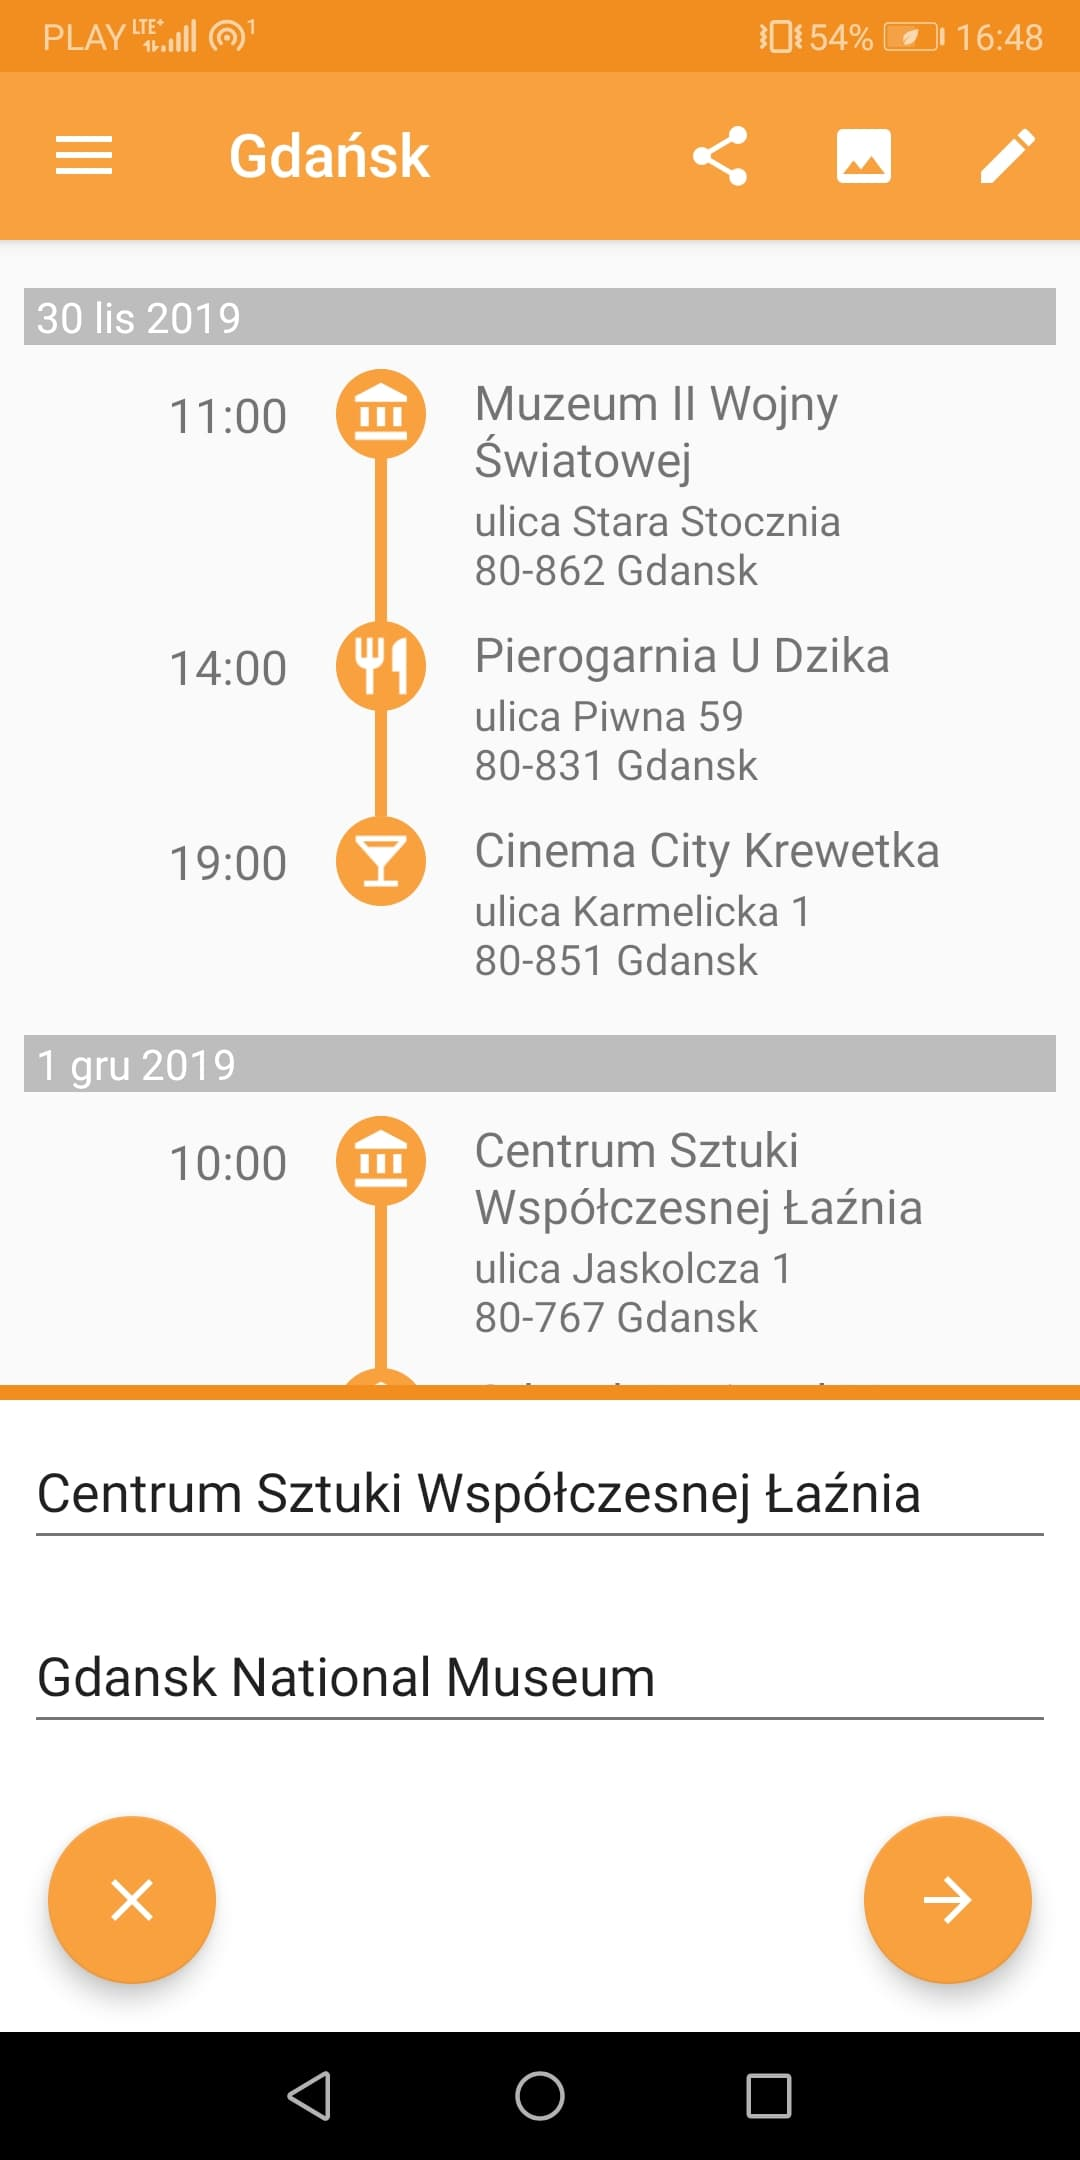
\includegraphics[width=0.9\linewidth, width=5cm]{transport1}
\label{fig:transport1}
\end{subfigure}
\begin{subfigure}{0.4\textwidth}
\centering
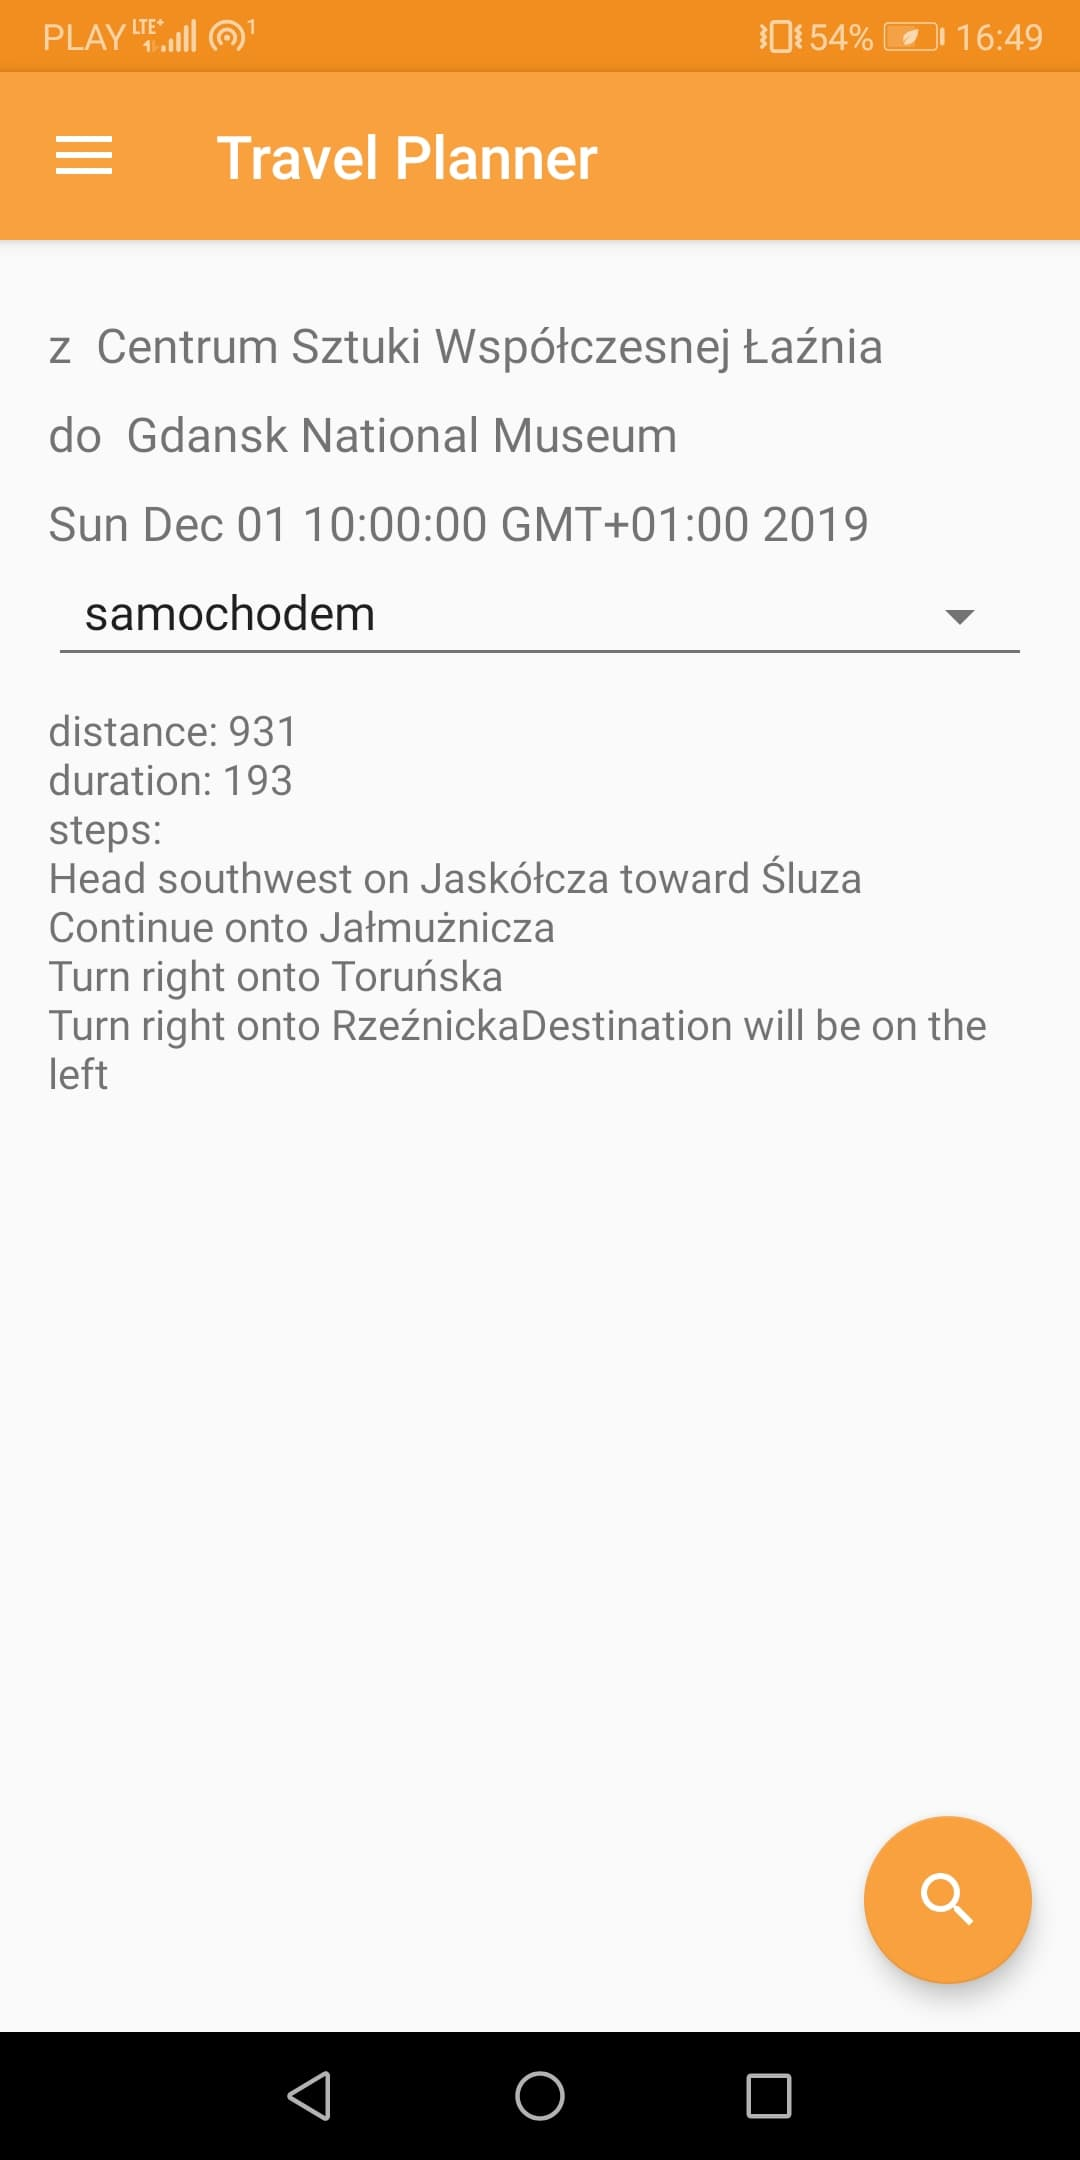
\includegraphics[width=0.9\linewidth, width=5cm]{transport2}
\label{fig:transport2}
\end{subfigure}
\caption{Wyszukiwanie transportu}
\label{fig:podrecznik12}
\end{figure}
\FloatBarrier


\section{Poszczególny element planu dnia}
Aplikacja umożliwia wykonywanie kilku czynności związanych z poszczególnym elementem planu dnia. Oprócz możliwości odczytania szczegółowych informacji na jego temat można ocenić dane miejsce, oznaczyć plan jako ukończony oraz udostępnić go w medium społecznościowym.

\begin{figure}[h]
\centering
\begin{subfigure}{0.4\textwidth}
\centering
\includegraphics[width=0.9\linewidth, width=5cm]{planElements}
\caption{Widok planu podróży}
\label{fig:planElements}
\end{subfigure}
\begin{subfigure}{0.4\textwidth}
\centering
\includegraphics[width=0.9\linewidth, width=5cm]{ratePlace2}
\caption{Ocenianie elementu planu}
\label{fig:ratePlace2}
\end{subfigure}
\caption{Pojedyncza podróż}
\label{fig:podrecznik4}
\end{figure}
\FloatBarrier


\subsection{Kliknięcie elementu}
Po kliknięciu na wybrany element pojawia się osobny widok zawierający dokładne informacje na temat wybranego miejsca. Istnieje możliwość wystawienia oceny.

\subsection{Przytrzymanie elementu}
Po przytrzymaniu palca na danym planu dnia pojawia się dymek z trzema opcjami do wyboru.

\begin{figure}[h]
\centering
\begin{subfigure}{0.3\textwidth}
\centering
\includegraphics[width=0.9\linewidth, width=5cm]{popUpMenu2}
\caption{Opcje elementu planu }
\label{fig:popUpMenu2}
\end{subfigure}
\begin{subfigure}{0.3\textwidth}
\centering
\includegraphics[width=0.9\linewidth, width=5cm]{deleteMode}
\caption{Tryb usuwania }
\label{fig:deleteMode}
\end{subfigure}
\begin{subfigure}{0.3\textwidth}
\centering
\includegraphics[width=0.9\linewidth, width=5cm]{popUpMenu}
\caption{Manualna realizacja planu}
\label{fig:popUpMenu}
\end{subfigure}
\caption{Przytrzymanie elementu planu}
\label{fig:podrecznik5}
\end{figure}
\FloatBarrier

\paragraph{Usuwanie elementu}
Po wybraniu opcji "Usuń" zostaje włączony tryb usuwania.
Jest on oznaczony jasnoszarym kolorem.
W celu usunięcia elementu należy:
\begin{enumerate}
\item Zaznaczyć wszystkie elementy, które mają być usunięte
\item Potwierdzić wykonanie czynności poprzez kliknięcie ikony kosza na śmieci
\end{enumerate}
\textbf{UWAGA Przejście do trybu usuwania jest możliwe w każdym widoku zawierającym listę elementów. Przejście do niego jest wykonywane po dłuższym przytrzymaniu jednego z elementów.}



\paragraph{Manualna realizacja planu}
\begin{enumerate}
\item W przypadku ukończonego planu zawiera tekst "Oznacz jako nieukończony"
\item W przypadku nieukończonego planu zawiera tekst "Oznacz plan jako ukończony"
\end{enumerate}
Ukończone elementy planu dnia mają zmniejszoną intensywność kolorów.


\paragraph{Udostępnianie w medium społecznościowym}
Gdy użytkownik ma zainstalowaną aplikację Facebook posiada możliwość udostępnienia elementu planu na swojej "tablicy". W celu wykonania tej czynności należy:
\begin{enumerate}
\item Nacisnąć opcję "Udostępnij"
\item Napisać treść posta
\end{enumerate}
Domyślna tekst zawiera link do wybranego miejsca na mapie HERE

\begin{figure}[h]
\begin{subfigure}{0.3\textwidth}
\centering
\includegraphics[width=0.9\linewidth, width=5cm]{shareOnFacebook}
\caption{Udostępnianie posta}
\label{fig:shareOnFacebook}
\end{subfigure}
\begin{subfigure}{0.7\textwidth}
\centering
\includegraphics[width=0.9\linewidth, width=9cm]{hereMobile}
\caption{Widok linku do map HERE}
\label{fig:hereMobile}
\end{subfigure}
\caption{Udostępnianie elementu planu}
\label{fig:podrecznik8}
\end{figure}
\FloatBarrier

\section{Skanowanie dokumentów}
Użytkownik posiadający plan podróży ma możliwość dodania skanu – czarno-białego zdjęcia z wyróżnionymi istotnymi informacjami.
W celu przechowania dokumentu w aplikacji należy:
\begin{enumerate}
\item Kliknąć na symbol hamburgera
\item W bocznym menu wybrać "Skany"
\item Nacisnąć przycisk zawierający symbol "+"
\item Wyrazić zgodę na dostęp do aparatu
\item Wykonać zdjęcie dokumentu
\item Wybrać interesujący obszar (dowolny czworokąt)
\item Zaakceptować przekształcenie obrazu klikając przycisk "Skanuj"
\item Miniatura skanu pojawi się w galerii
\end{enumerate}


\begin{figure}[h]
\begin{subfigure}{0.5\textwidth}
\centering
\includegraphics[width=0.9\linewidth, width=5cm]{sideBar}
\caption{Boczne menu}
\label{fig:sideBar}
\end{subfigure}
\begin{subfigure}{0.5\textwidth}
\centering
\includegraphics[width=0.9\linewidth, width=5cm]{scans}
\caption{Galeria skanów}
\label{fig:scans}
\end{subfigure}
\begin{subfigure}{0.5\textwidth}
\centering
\includegraphics[width=0.9\linewidth, width=5cm]{chooseScan}
\caption{Wybranie ważnych informacji}
\label{fig:chooseScan}
\end{subfigure}
\begin{subfigure}{0.5\textwidth}
\centering
\includegraphics[width=0.9\linewidth, width=5cm]{scan}
\caption{Obraz po przekształceniu}
\label{fig:scan}
\end{subfigure}
\caption{Wykonanie skanu}
\label{fig:podrecznik8}
\end{figure}
\FloatBarrier

\section{Znajomi}
Chcąc udostępnić innemu użytkownikowi podróży należy go wcześniej dodać do znajomych. Można to zrobić w następujących krokach:
\begin{enumerate}
\item Kliknąć na symbol hamburgera
\item W bocznym menu wybrać "Znajomi"
\item Wpisać w wyszukiwarce adres mailowy danego użytkownika
\item Wybrać odpowiedni mail z podpowiedzi
\item Potwierdzić chęć dodania do znajomych, poprzez kliknięcie "OK"
\item W przypadku prawidłowego wykonania czynności użytkownik zostanie automatycznie dodany do listy znajomych oraz pojawi się odpowiednie powiadomienie
\end{enumerate}

\begin{figure}[h]
\begin{subfigure}{0.3\textwidth}
\centering
\includegraphics[width=0.9\linewidth, width=5cm]{friends1}
\caption{Wyszukiwanie znajomych}
\label{fig:friends1}
\end{subfigure}
\begin{subfigure}{0.3\textwidth}
\centering
\includegraphics[width=0.9\linewidth, width=5cm]{friends2}
\caption{Potwierdzenie decyzji}
\label{fig:friends2}
\end{subfigure}
\begin{subfigure}{0.3\textwidth}
\centering
\includegraphics[width=0.9\linewidth, width=5cm]{friends3}
\caption{Wynik czynności}
\label{fig:friends3}
\end{subfigure}
\caption{Dodawanie znajomych}
\label{fig:podrecznik9}
\end{figure}
\FloatBarrier


\section{Rekomendacja miejsc}
Bazując na opiniach innych użytkowników aplikacja wyświetla listę polecanych miejsc. W trakcie korzystania z aplikacji użytkownik:
\begin{enumerate}
\item Dostaje powiadomienie o znalezieniu miejsc wartych jego uwagi
\item Klika na powiadomienie od aplikacji
\item Zostaje przekierowany do aplikacji z wyświetlonym oknem zawierającym listę rekomendowanych miejsc
\end{enumerate}
\begin{figure}[h]
\centering
\begin{subfigure}{0.4\textwidth}
\centering
\includegraphics[width=0.9\linewidth, width=5cm]{recomendation1}
\caption{Powiadomienie aplikacji}
\label{fig:recomendation1}
\end{subfigure}
\begin{subfigure}{0.4\textwidth}
\centering
\includegraphics[width=0.9\linewidth, width=5cm]{recomendation2}
\caption{Lista miejsc wartych uwagi}
\label{fig:recomendation2}
\end{subfigure}
\caption{Rekomendacja atrakcji}
\label{fig:podrecznik11}
\end{figure}
\FloatBarrier

\chapter{Podsumowanie (Anna Malizjusz)}

\par Wynikiem pracy inżynierskiej jest zaimplementowana, działająca w środowisku testowym aplikacja mobilna oraz serwer REST. Zrealizowane zostały wszystkie wymagania o wysokim priorytecie niezbędne do akceptacji projektu. Najważniejsze z nich to:
\begin{itemize}
\item rejestracja i logowanie użytkownika,
\item dodanie, przeglądanie i edycja planu podróży i planu dnia,
\item wyszukanie elementu w pobliżu danej lokalizacji, w szczególności zakwaterowania,
\item wyszukanie innego użytkownika i udostępnienie mu podróży,
\item dodanie oceny do odwiedzonego miejsca,
\item otrzymanie propozycji na podstawie ocen,
\item wyszukanie transportu między lokalizacjami,
\item skanowanie biletów.
\end{itemize}

\par Zaimplementowano też kilka dodatkowych funkcji, takich jak udostępnienie odwiedzonego miejsca w serwisie Facebook oraz oznaczenie planu dnia jako wykonany. Uwzględniano ostrzeżenia o użyciach przestarzałych funkcji, aby w aplikacji korzystano z najnowszych i najbezpieczniejszych praktyk.

\par Aplikację mobilną przetestował zespół programistów oraz kilku testerów. Nie stwierdzono rażących błędów, które uniemożliwiałyby korzystanie z zaimplementowanego rozwiązania. Interfejs okazał się łatwy w obsłudze dla młodych ludzi.

\par W trakcie projektu inżynierskiego zespół doświadczył trudności w implementacji rozwiązania "od zera", bez bazowego kodu ani dokładnych. Brakowało również praktyki w prowadzeniu względnie obszernego i skomplikowanego przedsięwzięcia, jakim jest stworzenie działającej aplikacji w pół roku. Wielokrotnie wybrane rozwiązania były uznawane za niewystarczające i zmieniane na lepsze. Początkowo tryb pracy i stosowane konwencje często się zmieniały, jednak w pierwszym etapie projektu udało się ustabilizować wewnętrzne wymagania. Dzięki temu recenzje kodu przebiegały sprawniej.

\par Spotykano się z problemem braku pomocnych informacji w internecie. Część używanych rozwiązań zostało oznaczonych jako przestarzałe i należało samodzielnie znaleźć aktualniejsze. Czasem część znalezionych informacji była specyficzna dla języka Java i nie istniała banalna konwersja do używanego języka Kotlin.

\par Podczas pracy nad aplikacją mobilną i serwerową zdefiniowano kolejne przydatne funkcjonalności lub ulepszenia istniejących. Postanowiono umożliwić użytkownikowi otrzymywanie powiadomień na adres email, a także umożliwić edycję planu dnia. Dodatkowo należy rozszerzyć aplikację o możliwość zmienienia oraz przypomnienia hasła. W serwisie GitHub stworzono nowe zadania odnośnie poprawienia jakości kodu obsługującego zapytania na serwerze, w bazie danych oraz w aplikacji mobilnej. Zdecydowano o przyszłej zmianie niektórych z elementów aplikacji, np. sposobu wyświetlania obiektów na mapie. Jednocześnie planowane jest zaimplementowanie kolejnych funkcjonalności, które zostały oznaczone jako mniej ważne.

\par Zdecydowano o późniejszym dokładniejszym pokryciu kodu testami jednostkowymi, a także o dodaniu większej liczby testów integracyjnych. W celu łatwiejszego i bezpieczniejszego rozwoju aplikacji zostaną zaimplementowane mechanizmy ciągłej integracji (ang. continous integration), które zapobiegną problemom z kompilacją oraz działaniem aplikacji na głównej gałęzi (ang. branch) repozytorium (master).

\par Zaimplementowane rozwiązanie, dzięki zachowaniu dobrych praktyk programistycznych podczas pisania kodu, może być dalej rozwijane w ramach pracy magisterskiej. Dotychczasowa praca zespołu zwiększyła jego umiejętności, zarówno programistyczne, jak i zdolność do współpracy z innymi członkami grupy.

\chapter*{Podział zadań implementacyjnych}
\addcontentsline{toc}{chapter}{Podział zadań implementacyjnych}

\captionof{table}{Autorzy zaimplementowanych funkcji\label{tab:autorzy}}

\centering
\begin{longtable}{ |p{3.3cm}|p{3.3cm}|p{3.3cm}|p{3.3cm}| }
\hline
\thead{Dorota Tomczak} & \thead{Magdalena Solecka} & \thead{Anna Malizjusz} & \thead{Karolina Makuch}\\

\hline
Zaprojektowanie i implementacja bazowej aplikacji mobilnej (wzorzec MVP, wstrzykiwanie zależności Dagger2)
& Wybór systemu zarządzania bazą danych Postgresql
& Projekt i implementacja bazowej postaci serwera oparta o framework Spring Boot 
& Implementacja wyświetlania znajomych oraz wyszukiwania użytkowników w celu dodania ich do znajomych \\

\hline
Obsługa sytuacji wyjątkowych na serwerze
& Implementacja podstawowego dostępu do bazy wyznaczającego schemat dla kolejnych modeli przy użyciu repository pattern
& Implementacja mechanizmów uwierzytelniania i autoryzacji na serwerze
& Implementacja manualnej realizacji planu \\

\hline
Implementacja skanera z użyciem OpenCV
& Pierwsza implementacja ekranu logowania i rejestracji
& Wyszukiwanie obiektów w aplikacji - implementacja wyboru miejsca z mapy
& Implementacja udostępniania planu podróży wybranym znajomym\\

\hline
Tworzenie planów podróży po stronie aplikacji (formularz dodawania i chronologiczne wyświetlanie listy)
& Dodawanie planów podróży po stronie serwera
& Wyświetlanie szczegółowych informacji o miejscu w planie dnia
& Implementacja udostępniania planu dnia w medium społecznościowym (Facebook)\\

\hline
Obsługa pobierania i przesyłania plików (skany i zdjęcia podróży)
& Implementacja testów automatycznych operacji dostępu do bazy danych
& Odczytywanie i korzystanie z informacji otrzymanych z Here API i Google API
& \\

\hline
Integracja w aplikacji komponentu \textit{Navigation drawer }
& Implementacja trybu usuwania w aplikacji mobilnej
& Komunikacja z serwerem w aplikacji mobilnej
& \\

\hline
Implementacja rekomendacji miejsc i wysyłanie ich w formie powiadomień
& Implementacja dodawania podróży oraz zmiany nazwy podróży
& Implementacja logiki rejestracji i logowania w aplikacji
& \\

\hline
Testy jednostkowe i instrumentalne dla logowania, rejestracji i komponentu \textit{launcher}
& 
& 
& \\

\hline
\end{longtable}


\bibliographystyle{plain}
\begin{thebibliography}{1}
\addcontentsline{toc}{chapter}{Bibliografia}
  \bibitem{Here} developer.here.com
  \bibitem{gms.location} developers.google.com/android/reference/com/google/android/gms/location/package-summary
  \bibitem{Android usage} gs.statcounter.com/android-version-market-share/mobile-tablet/worldwide
  \bibitem{SearchView} https://developer.android.com/reference/android/widget/SearchView
  \bibitem{ContentProvider} https://developer.android.com/reference/android/content/ContentProvider
  \bibitem{SlidingUpPanelLayout} https://github.com/umano/AndroidSlidingUpPanel
  \bibitem{Spring documentation} https://docs.spring.io/spring-boot/docs/current/reference/htmlsingle/
  \bibitem{JWT} https://tools.ietf.org/html/rfc7519
  \bibitem{JWT library} https://mvnrepository.com/artifact/io.jsonwebtoken/jjwt
  \bibitem{Retrofit library} https://square.github.io/retrofit/
  \bibitem{OkHttpClient} https://square.github.io/okhttp/
  \bibitem{Dagger 2} https://github.com/google/dagger
  \bibitem{SimpleDocumentScanner-Android} https://github.com/jbttn/SimpleDocumentScanner-Android
  \bibitem{OpenCV} https://opencv.org/
  \bibitem{FacebookBug} https://developers.facebook.com/support/bugs/332619626816423/
  \bibitem{mobileHere} https://mobile.here.com/
  \bibitem{Glide} https://bumptech.github.io/glide/
  \bibitem{Apache Mahout} https://mahout.apache.org/
  \bibitem{Postman} https://www.getpostman.com/
  \bibitem{Firebase} https://firebase.google.com/docs/cloud-messaging
  \bibitem{HereApi} https://developer.here.com/
  \bibitem{GoogleApi} https://cloud.google.com/maps-platform/routes/
  \bibitem{JsonParser} https://static.javadoc.io/com.google.code.gson/gson/2.8.5/com/google/gson/JsonParser.html
  \bibitem{GsonBuilder} https://static.javadoc.io/com.google.code.gson/gson/2.8.0/com/google/gson/GsonBuilder.html
  \bibitem{escapeUtils} https://commons.apache.org/proper/commons-lang/apidocs/org/apache/commons/lang3\\/StringEscapeUtils.html
  \bibitem{JUnit} https://junit.org/junit4/
  \bibitem{JUnitParams} https://github.com/Pragmatists/JUnitParams
  \bibitem{MockK} https://mockk.io/
  \bibitem{RxJava} https://github.com/ReactiveX/RxJava
  \bibitem{Espresso} https://developer.android.com/training/testing/espresso
  \bibitem{MockK-Android} https://mockk.io/ANDROID.html
  \bibitem{Google I/O 2019} https://techcrunch.com/2019/05/07/kotlin-is-now-googles-preferred-language-for-android-app-development/
  \bibitem{ImageView} https://developer.android.com/reference/android/widget/ImageView
\end{thebibliography}


\listoffigures
\listoftables

\end{document}
